\documentclass{report}
\usepackage[utf8]{inputenc}
\usepackage{amsmath}
\usepackage{afterpage}
\usepackage{amssymb}
\usepackage{svg}
\usepackage{listings}
\usepackage{float}
\usepackage{graphicx,wrapfig,lipsum}
\usepackage[makeroom]{cancel}
\usepackage{blindtext}
\usepackage{multicol}
\usepackage{hyperref}
\usepackage{eurosym}


\begin{document}

\begin{titlepage}
    \begin{center}
        \vspace*{1cm}

        \huge
        \textbf{Sistemi elettronici programmabili}

        \vspace{0.5cm}

        Appunti del corso presso l'Università di Pisa

        \vspace{1.5cm}

        \textbf{Aleandro Prudenzano}

        \vfill
        \vspace{0.8cm}

        A.A. 2021-2022

    \end{center}
\end{titlepage}

\clearpage
\begingroup
  \pagestyle{empty}
  \null
  \newpage
\endgroup

\renewcommand{\contentsname}{Indice}
\tableofcontents

\clearpage
\begingroup
  \pagestyle{empty}
  \null
  \newpage
\endgroup

\chapter{Introduzione}
\section{Introduzione}
La crittografia (scrittura nascosta) è lo studio \emph{delle tecniche matematiche per mascherare i messaggi} a differenza della \emph{crittoanalisi} che tenta di svelarli.
Esiste un termine più generico che li comprende: \emph{crittologia}.
Il tipico scenario in cui ci poniamo è quello in cui Alice e Bob vogliono comunicare un messaggio \emph{m} su un canale insicuro in cui è possibile intercettare i messaggi. Decidono quindi di adottare un metodo di cifratura che trasforma m in \emph{c}, detto \emph{crittogramma} che deve essere:

\begin{itemize}
    \item \emph{incomprensibile} al crittoanalista (Eve - Eavesdropper d'ora in poi)
    \item \emph{facilmente decifrabile} da Bob
\end{itemize}

\subsection{Cifratura}
L'operazione con la quale si trasforma m in c è di fatto una funzione:
$$
    C: msg \longrightarrow critto
$$

\subsection{Decifratura}
L'operazione inversa:
$$
    D: critto \longrightarrow msg
$$

\subsection{Schema di comunicazione}
$$
    Alice: m \xrightarrow{C} c \xrightarrow[\text{canale insicuro}]{c} c \xrightarrow{D} m :Bob
$$
Si noti che per funzionare \emph{C} e \emph{D} devono essere in tempo polinomiale mentre per il crittoanalista, noto \emph{c}, deve essere esponenziale il tempo utile per riottenere \emph{m}.
NB: \emph{C} e \emph{D} devono essere l'una l'inversa dell'altra:
$$
    D(c) = D(C(m)) = m
$$
quindi \emph{C} è iniettiva: m diversi vanno in c diversi.

\subsection{Esempi antichi}
Erodoto in "Storie" (V secolo a.C.) scrive:
si prende un servitore, si rasano i suoi capelli e si scrive il messaggio sulla sua testa, si aspetta che la ricrescita lo copra e poi si spedisce il servitore verso Bob che dovrà solamente rasarlo nuovamente.

Gli spartani (V secolo a.C.) usavano lo scitale che è un'asta cilindrica costruita in due esemplari identici posseduti dai due corrispondenti. Su un pezzo di pelle viene scritto il messaggio dopo averlo avvolto attorno al cilindro seguendo le linee di esso. La fettuccia viene poi fatta indossare da un'uomo che la porta al ricevente.

Enea Tattico (Grecia, IV Secolo a.C.) dedica un intero capitolo ai metodi militari usati per scambiarsi i messaggi:
\begin{itemize}
    \item inviare un libro con alcune lettere sottolineate a formare il messaggio in chiaro
    \item sostituire le vocali con altri simboli
\end{itemize}

Cifrario di Cesare: è il più antico cifrario di concezione moderna. \emph{c} è ottenuto da \emph{m} sostituendo ogni lettera con quella a 3 posizioni più avanti:
$$ A \longrightarrow D $$
$$ B \longrightarrow E $$
$$ C \longrightarrow F $$
$$ D \longrightarrow G $$
$$ .. \longrightarrow .. $$
La segretezza in questo caso dipende dalla conoscenza del metodo quindi era destinato ai soli utilizzi ristretti.

\subsection{Livello di segretezza}
I metodi crittografici si classificano in:
\begin{itemize}
    \item \emph{per uso ristretto}: in cui la parte segreta del meccaniscmo è ampia (C e D sono tenute segrete)
    \item \emph{per uso generale}: in cui la parte segreta è molto limitata (si restringe alla sola \emph{chiave}, nota solo ai due endpoint della comunicazione)
\end{itemize}
NB: per i cifrari di massa quindi le regole sono pubblcihe, solo le chiavi sono segrete. Occorre sempre pensare che il nemico conosca il sistema.

Ridefiniamo quindi:
$$ c = C(m, k) $$
$$ m = D(c, k) $$
con \emph{k} chiave segreta diversa per ogni coppia di utenti.
Se non si conosce \emph{k} la conoscenza dell'algoritmo non deve permettere l'estrazione di informazioni dal crittogramma. Se una chiave viene divulgata basta generarne un'altra lasciando inalterati \emph{C} e \emph{D}.
Ovviamente l'insieme delle chiavi deve esere così grande da non essere rompibile tramite brute-force e deve essere scelta in modo casuale.

NB: brute-force $\equiv$ \emph{attacco esauriente}

Es: se |key| = $10^{20}$ ed un calcolatore impiegasse $10^{-6}$ secondi per calcolare $D(c, k)$ e verificarne la significatività occorrerebbero comunque milioni di anni per provarle tutte.
NB: solo la grandezza dello spazio delle chiavi non è un buon indice per l'affidabilità di un cifrario, potrebbe sempre essere rotto matematicamente.

\subsection{Crittoanalisi}
\begin{itemize}
    \item comportamento \emph{passivo}: ci si limita ad ascoltare il canale
    \item comportamento \emph{attivo}: si disturbano le comunicazioni o si modifica il contenuto dei messaggi
\end{itemize}
Gli attacchi dipendono dalle informazioni in possesso del crittoanalista:
\begin{itemize}
    \item \emph{cipher text attack}: si hanno una seria di testi cifrati: $ c_{1}, \_ , c_{r} $
    \item \emph{known plain-text attack}: il crittoanalista ha delle coppie
    $$(m_{1}, c_{1}), \_ , (m_{r}, c_{r})$$
    \item \emph{chosen plain-text attack}: ci si procura una serie di coppie
    $$(m_{1}, c_{1}), \_ , (m_{r}, c_{r})$$
    relative a messaggi in chiaro scelti.
\end{itemize}

\subsection{Attacchi man-in-the-middle}
Il crittoanalista si installa sul canale ed interrompe le comunicazioni dirette tra i due, le sostituisce con messaggi propri e convince ogni utente che quei messaggi provengono legittimamente dall'altro.

\subsection{Situazione attuale}
Si conoscono alcuni \emph{cifrari perfetti} ma richiedono operazioni estremamente complesse, quindi sono utilizzati in condizioni estreme. La definizione di cifrario inattaccabile si deve a \emph{Claude Shannon} ('45 ma pubblicato nel '49). Il messaggio in chiaro ed il crittogramma sono completamente scorrelati tra loro. un esempio è il \emph{one-time pad} che richiede:
\begin{itemize}
    \item una chiave diversa per ogni messaggio
    \item perfettamente casuale
    \item lunga quanto il messaggio
\end{itemize}
Come vanno generate? Come vanno scambiate?
I cifrari utilizzati oggigiorno non sono perfetti ma sono comunque \emph{dichiarati sicuri} perché inviolati e per violarli è necessario risolvere problemi matematici estremamente difficili (abbiamo solo algoritmi esponenziali) quindi è richiesto tanto tempo o calcolatori molto grandi, nella pratica impossibile.

NB: non sempre è noto se l'algoritmo esponenziale è l'unico metodo o ce ne sono altri ancora non scoperti.

Uno dei cifrari di oggi è l'\emph{AES} (Advanced Encryption Standard): è lo standard per le comunicazioni non classificate, pubblicamente noto ed implementabile. Usa chiavi brevi a 128 o 256 bit. E' un cifrario simmetrico a blocchi, la stessa chiave quindi si usa sia per cifrare che per decifrare.

NB: la chiave non è scelta dai partecipanti ma dai compter che usano.
Come trasmettere le chiavi in maniera sicura ed evitare che venga intercettata?

\subsection{Distribuzione delle chiavi}
Nel 1976 è stato proposto un protocollo di creazione e scambio di chiavi su un canale insicuro scenza la necessità che le due parti debbano essersi scambiate altre informazioni. Questo algoritmo è detto \emph{protocollo Diffie-Hellman} acora osa usato largamente.

NB: inventato da Merkle e poi da Diffie ed Hellman

Questi stessi hanno anche creato il concetto di crittografia a chiave pubblica senza tuttavia averne già una implementazione.

\subsection{Cifrari simmetrici ed asimmetrici}
Nei cifrari simmetrici la chiave è unica ed usata sia per criptare che per decriptare ed è nota solo ai due partner che devono averla concordata su un canale sicuro.
Nei cifrari asimmetrici invece si usano una coppia di chiavi:
\begin{itemize}
    \item \emph{$K_{pub}$}: si usa per cifrare, è pubblica e nota a tutti
    \item \emph{$K_{priv}$}: è privata e nota solo a chi riceve.
\end{itemize}
Bisogna quindi creare delle coppie di chiavi per ogni persona che vuole comunicare. Più precisamente:
$$ c = C(m, K_{pub}) $$
$$ m = D(c, K_{priv}) $$
I sistemi simmetrici si dicono anche a chiave privata, mentre quelli asimmetrici si dicono a chiave pubblica.
Per usare un meccanismo come crittografia asimmetrica è necessario l'uso di funzioni \emph{one-way trapdoor} cioè passare da \emph{m} a \emph{c} è facile ma decifrare \emph{c} (senza conoscere la chiave) è difficile.

\subsection{RSA}
Nel 1977 Rivest-Shamir-Adleman inventano un sistema a chiave pubblica basato sulla difficoltà di fattorizzare grandi numeri in fattori primi.
Usando un sistema a chiave pubblica si ha una comunicazione molti a uno in quanto tutti hanno $K_{pub}$ e possono quindi cifrare i messaggi, ma solo il destinatario può leggerli conoscendo $K_{priv}$. Altri vantaggi sono:
\begin{itemize}
    \item tra n persone le chiavi sono $2n$, con un cifrario simmetrico invece sarebbero $\frac{n(n-1)}{2}$
    \item non è necessario lo scambio segreto di chiavi
\end{itemize}

Tuttavia sono molto più lenti e le chiavi sono molto lunghe. Sono soggetti ad attacchi di tipo testo in chiaro scelto.

\subsection{Cifrari ibridi}
Si usa un cifrario a chiave segreta per la comunicazione di massa ma la chiave viene scambiata tramite cifrari asimmetrici. Si hanno quindi:
\begin{itemize}
    \item chiavi piccole
    \item chiave simmetrica randomica impossibile da prevedere tramite attacco di tipo testo in chiaro scelto
\end{itemize}

\subsection{Applicazioni moderne}
Attualmente i protocolli crittografici sono usati anche per:
\begin{itemize}
    \item \emph{identificazione dell'utente}: si accerta l'identità
    \item \emph{autenticazione dell'utente}: si accerta che il messaggio venga dalla persona che dice di averlo mandato
    \item \emph{firma digitale}: permette di evitare che un utente che ha inviato un messaggio neghi di averlo fatto e si dimostra l'identità del mittente agli occhi del ricevente
\end{itemize}

\subsection{Svolte future}
\begin{itemize}
    \item trasmissione protetta sulla rete (OpenSSL)
    \item moneta elettronica (protocollo Bitcoin)
    \item protocolli zero-knowledge
    \item protocolli di cifratura quantistici
\end{itemize}
\section{Architetture}

\subsection{Architettura di Von Neumann}
La struttura generale di Von Neumann prevede:

\begin{figure}[H]
    \centering
    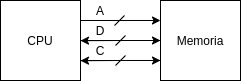
\includegraphics[width=150px]{images/2_Architetture/Von_Neumann.png}
\end{figure}

\begin{itemize}
    \item CPU: central processing unit, si occupa di prendere le istruzioni, decodificarle ed eseguirle
    \item Memoria: contiene i dati e le istruzioni
    \item A: sono i fili di indirizzo, emessi dalla CPU e ricevuti dalla memoria
    \item D: sono i fili di dato, sia la CPU che la memoria possono emettere dati, ovviamente non allo stesso tempo
    \item C: sono i fili di controllo, varia in dimensioni in base alle architetture. Alcuni fili importanti sono il memory\_read, il memory\_write, il segnale di memory\_wait, ecc
\end{itemize}

Alla fine tutto è un numero, anche le istruzioni per la CPU quindi anche le istruzioni possono andare in memoria per Von Neumann.

\subsection{Memoria}
La memoria è genericamente rappresentata come segue:
\begin{figure}[H]
    \centering
    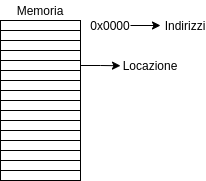
\includegraphics[width=150px]{images/2_Architetture/Memoria.png}
\end{figure}
Si tratta di un insieme di celle dette \emph{locazioni} di memoria, ognuna delle quali ha un \emph{indirizzo}.
Useremo l'esadecimale per indicare gli indirizzi in quanto è semplice convertirli in binario.
Per accedere ad una locazione la CPU emette l'indirizzo sul bus A, se deve scrivere pone anche un dato sul bus D e da il comando di memory\_write, se invece deve leggere pone il comando di memory\_read e campiona il bus D.

Ogni cella è composta da 8 bit per motivi storici: sono abbastanza per memorizzare un singolo carattere secondo la codifica ASCII; ne basterebbero 7 ma è un numero dispari ed anche primo, cosa molto brutta.

Per alcune applicazioni 8 bit possono essere pochi quindi alcuni calcolatori hanno memoria con locazioni di 16 bit, 32 bit, 64 bit.

\subsection{Architettura Harvard}
Per migliorare l'efficienza su alcuni task specifici conviene mettere due memorie separate e di diverso tipo: in questo modo nasce l'architettura Harvard:
\begin{figure}[H]
    \centering
    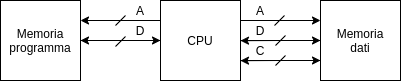
\includegraphics[width=300px]{images/2_Architetture/Harvard.png}
\end{figure}
 L'architttura Harvard è largamente usata per applicazioni DSP - \emph{Digital Signal Processing}, cioè operazioni velocissime e sempre uguali su dati in tempo reale.

\subsection{Comparazione}
\begin{table}[ht]
    \centering
    \begin{tabular}{c|c|c|c|c}
        & Flash & RAM & ALU & Architettura\\
        \hline
        AVR Mega & 128k & 8k & 8bit & Harvard \\
        MSP430 & 65k & 8k & 16bit & Von Neumann \\
        ARM & 1M & 96k & 32 bit & Von Neumann 
    \end{tabular}
\end{table}
\section{Architettura dell'ATmega32}
L'ATmega32 ha una architettura di tipo Harvard. In particolare abbiamo:
\begin{figure}[H]
    \centering
    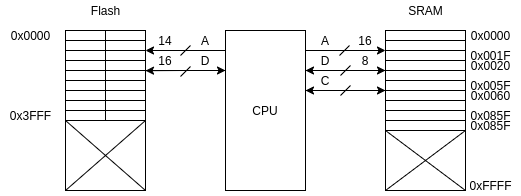
\includegraphics[width=330px]{images/3_Architettura_ATmega32/ATmega32.png}
\end{figure}

\subsection{Struttura della flash}
La memoria flash è composta da 16k righe di 16 bit, oppure 32k righe da 8 bit.
Questo 32k da il nome al microcontrollore.
Dato che gli accessi sono fatti a 16 bit sarebbe più corretto dire che la memoria è composta da 16 Kword piuttosto che da 32 Kbyte.
La memoria flash è occupata dal programma!

E' implementata dall'indirizzo 0x0000 fino all'indirizzo 0x3FFF, il resto dello spazio di indirizzamento è lasciato per utilizzi futuri. Si noti infatti che i bit di indirizzo sono 14 e non 16.

\subsection{Struttura della SRAM}
La SRAM può essere letta e scritta a piacere, è di fatto una RAM, quindi memoria volatile.
La memoria SRAM è più costosa in termini di transistori (6 transistori rispetto a 1 della flash), più grande sul chip ma è veloce. E' organizzata in celle da 8 bit ed è così segmentata:
\begin{itemize}
    \item 0x0000 - 0x001F: copia dei registri
    \item 0x0020 - 0x005F: periferiche
    \item 0x0060 - 0x085F: RAM
    \item 0x0860 - 0xFFFF: non implementata
\end{itemize}

Tra le periferiche si hanno i pin GPIO, cioè una periferica che si connette da una parte allo spazio di memoria e dall'altra ha dei pin che possono essere impostati a livello logico alto o a livello logico basso, sono utilizzati per interagire con il mondo esterno. Altre periferiche sono periferiche di comunicazione (SPI, I$^{2}$C, ecc).

Questo modello è detto \emph{I/O mappato in memoria} in quanto appunto le periferiche sono accessibili come fossero vera e propria memoria.

NB: se scrivo nella memoria non connessa è come se non avessi fatto niente, se leggo da quegli indirizzi leggo 0xFF, si dice che \emph{fallisce in silenzio}.


\subsection{CPU}
Le componenti fondamentali della CPU sono:
\begin{itemize}
    \item Decodificatore delle istruzioni: una volta letta l'istruzione dalla flash si occupa di decifrarla e configurare lo stato interno del processore per eseguirla.
    \item ALU: è l'unità aritmetico-logica, si occupa di eseguire le operazioni matematiche (somma, differeza, shift, ecc) e quelle logiche (comparazione, or, and). Non ha la moltiplicazione.
    \item Moltiplicatore: è un aggiunta alla ALU per poter eseguire le moltiplicazioni. E' stato aggiunto nella versione Mega dell'architettura.
    \item Registri r0-r31: sono memorie interne al processore da 1 byte, sono memorie volatili. Le operazioni di manipolazione dei dati vanno fatte esclusivamente all'interno dei registri, quindi servono e ne servono molti. Questi registri sono anche copiati in memoria, modificando un registro modifico la memoria, modificando la memoria modifico i registri:
    \begin{verbatim}
        MOV r7, r9          # copia r9 in r7
        STS 0x0007, r9      # scrivi r9 all'indirizzo 0x0007
    \end{verbatim}
    fanno la stessa cosa!
    La lettura dai registri non è distruttiva, la scrittura invece sovrascrive il valore precedente con quello nuovo!
\end{itemize}




\chapter{Programmazione in assembly}
\section{Status Register}
Uno dei registri interni al processore è lo \emph{Status Register}, si compone di 8 bit ognuno dei quali ha un significato e descrive una caratteristica dello stato interno del processore.

\begin{figure}[H]
    \centering
    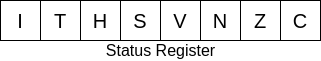
\includegraphics[width=250px]{images/4_Status_register/status_register.png}
\end{figure}

Questo registro può essere letto per intero leggendo l'ultimo indirizzo dello spazio delle periferiche.

\subsection{Carry bit}
Il bit meno significativo dello status register è detto \emph{carry bit} o \emph{carry flag} ed indica se c'è stato un riporto durante una somma o un presito durante una sottrazione.

La ALU prende quasi sempre due parametri (solo uno quando fa una negazione dei bit o cambia di segno) e restituisce un solo risultato, le operazioni con la ALU inoltre sono distruttive in quanto scrivono il risultato all'interno del registro usato come destinazione:

\begin{verbatim}
    ADD r7, r9  #  r7 <- r7 + r9
\end{verbatim}

La ALU fornisce un risultato a 8 bit, tuttavia è in grado di prendere il nono bit in uscita dalla somma richiesta e di aggiornare il carry flag, quindi il CF diventa 1 se la somma non è rappresentabile su 8 bit.

Anche nella sottrazione questo flag viene aggiornato, in particolare nella differenza A-B se A è minore di B allora il carry flag indica che c'è stato un prestito. Nella pratica quello che viene eseguito dalla ALU è:
$$ 12 - 17 = (256 + 12) - 17 = 251 $$
251 è il valore -5 espresso in complemento a 2.

Oltre che per il riporto o il prestito il CF può essere utilizzato per eseguire operazioni su più byte: 1000 non è rappresentabile su un singolo byte, possiamo pertanto suddividerlo in una parte alta ed in una parte bassa:
$$ 1000 - 248  = \text{0x03E8} - \text{0x00F8} $$

\begin{verbatim}
    MOV r1, 0x03 # r1 <- 0x03
    MOV r0, 0xE8 # r0 <- 0xE8
    # indico con r1:r0
    
    MOV r3, 0x00 # r3 <- 0x00
    MOV r2, 0xF8 # r2 <- 0xF8
    # indico con r3:r2
    
    SUB r0, r2   # r0 <- r0 - r2
    SBC r1, r3   # r1 <- r1 - r3 - CF
\end{verbatim}
usando l'istruzione SBC - \emph{subtract with carry} abbiamo scomposto una operazione su 16 bit in operazioni su 8 bit, questo possiamo scalarlo anche per operazioni a 32 bit e così via.

Per eseguire la stessa cosa con una somma esiste l'istruzione ADC - \emph{add with carry}.

\subsection{Zero bit}
Il secondo bit indica se l'ultima operazione aritmetica ha generato un risultato composto da tutti 0.
\begin{verbatim}
    MOV r7, 11
    MOV r8, 11
    SUB r7, r8 # il risultato è zero quindi Z = 1
\end{verbatim}

Possiamo usarlo per eseguire test di uguaglianza, se facendo una sottrazione lo zero flag va ad 1 allora i numeri erano uguali. La sottrazione tuttavia è distruttiva, per fare le comparazioni quindi esiste un'altra istruzione: CP, fa una sottrazione, aggiorna i flag dello SREG ma butta via il risultato anziché sovrascrivere il registro.
\begin{verbatim}
    CP r7, r8
\end{verbatim}

Un altro utilizzo lo si ha nel controllare se un bit ha un determinato valore, i microcontrollori hanno delle periferiche per leggere valori digitali dall'esterno, supponiamo pertanto di avere questo circuito:

\begin{figure}[H]
    \centering
    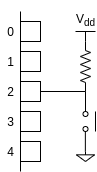
\includegraphics{images/4_Status_register/example_and_1.png}
\end{figure}
e di aver letto il valore dei pin nel registro r7 (vedremo come si fa più avanti). Il terzo bit di questo registro ora ha il valore del pin, vogliamo pertanto isolare quel singolo bit e sapere che valore ha: applichiamo una maschera eseguendo l'AND logico:
\begin{figure}[H]
    \centering
    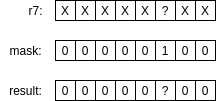
\includegraphics[width=150px]{images/4_Status_register/example_and_2.png}
\end{figure}

\begin{verbatim}
    # in r7 abbiamo il valore dei pin
    MOV r9, 0x04
    AND r9, r7
\end{verbatim}
ho quindi isolato il bit 2 ed inoltre ha aggiornato i flag, controllando lo Z flag posso trovarvi 1: ho quindi prodotto uno zero ed il pulsante era chiuso, oppure potrei trovarvi 0: in tal caso il pin era ad 1 e quindi il pulsante era aperto.

\subsection{Half carry bit}
Il bit H dello SREG indica se nell'ultima operazione aritmetica si è generato un half carry. Un half carry è un riporto che va dal terzo bit al quarto bit:

\begin{figure}[H]
    \centering
    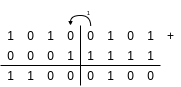
\includegraphics[width=150px]{images/4_Status_register/half_carry.png}
\end{figure}
questo flag è utile solo nelle operazioni con codifica BCD.

\subsubsection{Binary Coded Digit}
La codifica BCD prevede l'uso di 4 bit per rappresentare le cifre decimali, si usando i numeri da 0 a 9 esattamente come fossero rappresentati in binario. Supponiamo di dover sommare due numeri a due cifre in questa codifica, possiamo distinguere 3 casi:
\begin{itemize}
    \item 15 + 13 = 28
    
    La somma con la ALU è corretta anche leggendola in BCD
    
    \item 15 + 16 = 2B
    
    La somma con la ALU non è corretta in quanto abbiamo che la seconda cifra non ha fatto il riporto verso la prima, possiamo accorgercene controllando le singole cifre e vedendo che è maggiore di 9. Possiamo aggiustarla semplicemente sommando 6 (tolgo 10 per prendere ciò che c'è in più e sommo 16 per il riporto).
    
    2B + 6 = 31

    \item 18 + 19 = 31
    
    La somma non è corretta ma sembra esserlo perché le cifre sono tutte rappresentabili in BCD.
    Non abbiamo modo di accorgerci dell'errore.
    Questo errore è correlato al riporto tra i primi quattro bit ed i secondi quattro, intercettando questo riporto possiamo accorgerci dell'errore e fixarlo.
    Per fixare anche qui mi basta aggiungere 6 in quanto è ciò che ha portato in più nella seconda cifra per fare il riporto.
\end{itemize}

\subsection{Bit S V N}
Se eseguo una somma interpretando i numeri come numeri con segno, quindi in complemento a 2, il carry bit non è affidabile:
$$ 100 + 100 = 0x64 + 0x64 = 0xC8 $$
questa somma non ha emesso carry ed il bit più significativo è 1 quindi ci segna che il numero è negativo ma non dovrebbe esserlo in quanto entrambi gli addendi sono positivi.

In questo caso non possiamo affidarci al carry flag per sapere se la nostra somma è andata a buon fine. Per queste situazioni esistono altri 3 flag:
\begin{itemize}
    \item N \emph{negative flag}: copia del bit più significativo prodotto dall'operazione aritmetica
    \item V \emph{overflow flag}: è il valore prodotto da $N \oplus C$ ed indica e il risultato è corretto leggendolo come complemento a 2.
    \item S \emph{sign flag}: ci dice quale sarebbe stato il segno se il risultato fosse stato coretto
\end{itemize}

\subsection{Bit T}
Questo bit non ha un significato specifico, può essere settato e resettato dall'utente utilizzando due istruzioni. Sta per \emph{temporary flag}.

\subsection{Interrupt bit}
Questo flag è settabile e resettabile dal programmatore, serve ad abilitare o disabilitare la logica di interruzione.
Di norma è a 0.


\section{Modi di indirizzamento}
Ci sono diversi modi per prendere i dati da utilizzare nei calcoli.

\subsection{Indirizzamenti}

\subsubsection{Indirizzamento a registro}
Se il dato si trova all'interno di un registro ci basterà specificare il nome del registro per poterlo utilizzare:
\begin{verbatim}
    ADD r7, r9 # r7 <- r7 + r9
\end{verbatim}

\subsubsection{Indirizzamento immediato}
Se il dato è disponibile a tempo di compilazione possiamo inserirlo direttamente nella istruzione.
Possiamo specificarlo solamente come operando sorgente, ovviamente.
Per indicare questo indirizzamento si aggiunge una "I" alla fine dell'istruzione:
\begin{verbatim}
    ANDI r17, 0x41 # r17 <- r17 AND 0x41
\end{verbatim}

I valori possono essere specificati in:
\begin{itemize}
    \item decimale, con e senza segno:
    \begin{verbatim}
        SUBI r17, 13
        SUBI r17, -13
    \end{verbatim}
    
    \item esadecimale, preceduto da "0x":
    \begin{verbatim}
        SUBI r17, 0xD
    \end{verbatim}
    
    \item binario, preceduto da "0b":
    \begin{verbatim}
        SUBI r17, 0b00001101
    \end{verbatim}
    
    \item espressioni da calcolare: solo se le espressioni sono calcolabili a tempo di assemblaggio
    \begin{verbatim}
        LDI r18, 5*3
        LDS r9, 0x0870 + 5
    \end{verbatim}
\end{itemize}


NB: le istruzioni ADDI e ADCI non esistono, bisogna ricorrere a SUBI e SBCI e cambiare di segno l'operando immediato.

\subsubsection{Indirizzamento diretto}
Questa architettura, essendo RISC, non supporta operazioni memoria-registro o registro-memoria, bisogna utilizzare una istruzione per caricare il valore all' interno di un registro e successivamente usare il registro per fare i calcoli.
\begin{verbatim}
    LDS r9, 0x0870  # legge il byte nella SRAM all'indirizzo 
                    # 0x0870 e ricopia in r9
                    
    STS 0x0870, r9  # scrive il byte contenuto in r9
                    # all'indirizzo 0x0870 della SRAM
\end{verbatim}

\begin{figure}[H]
    \centering
    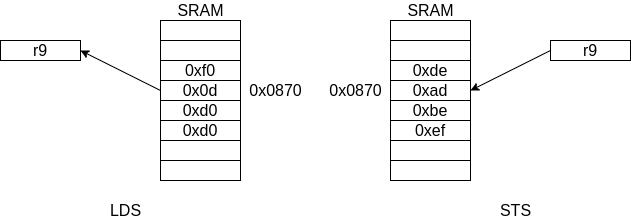
\includegraphics[width=300px]{images/5_Indirizzamento/LDS_STS.png}
\end{figure}

\subsubsection{Indirizzamento diretto con registro puntatore}
Esistono degli alias per alcune coppie di registri:
\begin{itemize}
    \item r31:r30 è identificato da Z
    \item r29:r28 è identificato da Y
    \item r27:r26 è identificato da X
\end{itemize}
queste coppie, e le relative label, sono usati per inserire degli indirizzi da usare per eseguire letture in memoria:
\begin{verbatim}
    LD r9, X  # legge dalla memoria all'indirizzo
              # contenuto in X
\end{verbatim}
Per inserire l'indirizzo nel registro X possiamo usare due modi:
\begin{verbatim}
    LDI r26, 0x70
    LDI r27, 0x08
        # utilizzando r27, r26
    
    LDI XL, 0x70
    LDI XH, 0x08
        # utilizzando gli alias
\end{verbatim}

Per accessi più complessi possiamo utilizzare alcuni operatori sui registri X, Y, Z:
\begin{verbatim}
    LD r10, X+  # legge da X ed incrementa X
            X-  # legge da X e decrementa X
            +X  # incrementa X e poi legge da X
            -X  # decrementa X e poi legge da X
\end{verbatim}

NB: non tutti e 3 i registri implementano tutte e 4 le modalità, il set di istruzioni \emph{non è ortogonale}!

Con il registro Y esiste anche:
\begin{verbatim}
    LD r11, Y + 4
        # legge all'indirizzo Y + 4
        # NON altera il contenuto di Y!
        # l'offset non può essere più grande di 6 bit
        # si possono usare negativi
\end{verbatim}




\section{Instruction set}
L'AVR esegue 1 istruzione per clock, non è propriamente così in quanto alcune istruzioni hanno necessità di più cicli di clock e tutte le istruzioni vogliono un clock per il fetch ed almeno uno per l'esecuzione.
E' vero però che sfruttando la pipeline a 2 livelli che la CPU ci mette a disposizione riusciamo ad eseguire 2 istruzioni in 2 cicli di clock, quindi in media abbiamo 1 istruzione per clock.

\subsection{Istruzioni aritmetiche}

\subsubsection{ADIW}
Somma un operando immediato a 16 bit ad una coppia di registri consecutivi:
\begin{verbatim}
    ADIW r10, 0x1010
        # Somma 0x1010 alla coppia di registri r11:r10
\end{verbatim}

\subsubsection{SBIW}
Sottrae un operando immedato a 16 bit ad una coppia di registri consecutivi:
\begin{verbatim}
    SBIW r10, 0x101
        # Sottrae 0x1010 alla coppia di registri r11:r10
\end{verbatim}

\subsubsection{MUL}
Esegue una moltiplicazione:
\begin{verbatim}
    MUL rx, ry
        # Esegue il prodotto tra i registri specificati
        # e pone il risultato in r1:r0
        # r1:r0 non possono essere usati per porci
        # i fattori
\end{verbatim}

NB: esistono diverse moltiplicazioni per i 3 casi possibili, in più quelli per i numeri in virgola fissa:
\begin{itemize}
    \item MUL: moltiplicazione tra numeri senza segno
    \item MULS: moltiplicazione tra numeri con segno
    \item MULSU: moltiplicazione tra un numeo signed ed uno unsigned
    
    \item MULF: moltiplicazione tra numeri in virgola fissa
\end{itemize}


\subsection{Istruzioni di salto}
\subsubsection{RJMP}
Quando il processore sta eseguendo le istruzioni mantiene l'indirizzo della prossima istruzione da eseguire nel registro Program Counter (PC), modificando questo registro possiamo eseguire dei salti.
L'istruzione RJMP prende come operando un numero, con segno, che indica quanto dobbiamo aggiungere al PC corrente per andare all'istruzione alla quale vogliamo saltare.
Nella pratica questa istruzione produce:
\begin{verbatim}
    PC <- PC + 1 + k
\end{verbatim}
l'aggiunta di 1 viene fatta alla fine della fase di fetch, successivamente si somma il $k$ specificato come operando.

\subsubsection{IJMP}
Salta all'indirizzo contenuto nel registro $Z$.
Compie un salto indiretto assoluto in quanto si deve specificare tutto l'indirizzo in $Z$ e non solo l'offset da sommare.

NB: i salti incondizionati ci mettono sempre 2 cicli interi in quanto il meccanismo di prefetch non può funzionare, va quindi invalidata la pipeline che porta a perdere un ciclo.

\subsubsection{JMP}
Salta all'indirizzo specificato come operando.
Questa istruzione ci mette 3 cicli di clock in quanto l'operando è a 16 bit ed in più deve sempre invalidare la pipeline.

\subsubsection{CPSE}
L'istruzione esegue una comparazione, dopodiché skippa l'istruzione seguente se gli operandi sono uguali.
\begin{verbatim}
    CPSE r0, r1
    JMP not_equal
    JMP equal
        # se r0 == r1 skippa il salto a not_equal
        # ed esegue quello a equal
\end{verbatim}

NB: la durata di questa istruzione dipende se skippa (invalidare la pipeline) o non skippa.

\subsubsection{BREQ - BRNE}
\begin{itemize}
    \item BREQ esegue il salto relativo se Zero flag = 1
    \item BREQ esegue il salto relativo se Zero flag = 0
\end{itemize}

Queste istruzioni di salto condizionato di solito sono precedute da una CP, quindi si riferiscono a quella comparazione.

\subsubsection{BRCS - BRCC}
\begin{itemize}
    \item BRCS esegue il salto relativo se Carry flag = 1
    \item BRCC esegue il salto relativo se Carry flag = 0
\end{itemize}

\subsubsection{BRSH - BRLO}
\begin{itemize}
    \item BRSH: alias per BRCC, salta se maggiore o uguale
    \item BRLO: alias per BRCS, salta se minore
\end{itemize}
Si usano per i numeri naturali.

\subsubsection{BRGE - BRLT}
\begin{itemize}
    \item BRGE: salta se maggiore o uguale
    \item BRLT: salta se minore
\end{itemize}
Si usano per numeri interi.


\subsection{Istruzioni per dialogare con le periferiche}
Abbiamo già visto come le periferiche siano inserite nello spazio di memoria tra gli indirizzi 0x0020 e 0x005F, possiamo dunque leggere e scrivere usando le istruzioni che abbiamo già visto come LDS - STS.
Tuttavia dato che la comunicazione con le periferiche è frequente esistono delle istruzioni un po' più specifiche: IN per leggere da una periferica e OUT per scrivere su una periferica.

Queste istruzioni prevedono l'utilizzo di un \emph{peripheral address} ottenuto semplicemente come: indirizzo reale - 0x0020.

Queste istruzioni sono inoltre più veloci dato che l'indirizzo è a 8 bit e possono accedere esclusivamente ad indirizzi nello spazio delle periferiche!

\begin{verbatim}
    LDS r9, 0x0020
    IN r9, 0x00
        # fanno la stessa cosa
        
    STS 0x0020, r9
    OUT 0x00, r9
        # fanno la stessa cosa
\end{verbatim}

\subsection{Operazioni sui bit}
\begin{itemize}
    \item SBI P, b: setta il b-esimo bit del registro P di I/O
    
    \item CBI P, b: pulisce il b-esimo bit del registro P di I/O
\end{itemize}

\subsubsection{Shift e rotazione}
\begin{itemize}
    \item LSL: shifta tutti i bit di un registro a sinistra, inseriscono il MSB nel CF ed uno 0 come LSB
    \begin{figure}[H]
        \centering
        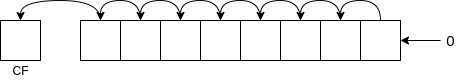
\includegraphics[width=250px]{images/6_Instruction_set/LSL.png}
    \end{figure}
    
    \item LSR: shifta tutti i bit di un registro a destra, inseriscono il LSB nel CF ed uno 0 come MSB
    \begin{figure}[H]
        \centering
        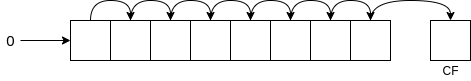
\includegraphics[width=250px]{images/6_Instruction_set/LSR.png}
    \end{figure}
\end{itemize}
Lo shift logico si usa per moltiplicare per 2 (a sinistra) o dividere per 2 (a destra).
Se il numero è con segno e lo moltiplico per due potrebbe non essere rapprsentabile, in tal caso il CF viene settato ad 1.

Nella divisione invece con segno il risultato dovrebbe essere sempre rappresentabile, tuttavia se inserisce lo 0 in testa questo non è più vero:

$$ -1: 11111111 \xrightarrow{} 011111111 : +127 $$
Per risolvere dovrei far entrare come bit più significativo una copia dello stesso MSB, esiste pertanto l' istruzione ASR:
\begin{figure}[H]
    \centering
    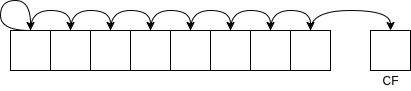
\includegraphics[width=250px]{images/6_Instruction_set/ASR.png}
\end{figure}
Ricopiare il MSB è detto \emph{estensione del segno}.
Questa operazione va fatta anche quando si vuole portare un numero con segno da 8 a 16 bit.

Si noti che dividere -1 con lo shift aritmetico a destra produce ancora -1.
Per definizione la divisione è:
$$ \frac{p}{q} \text{ tc } nq + r = p $$
con $n,r$ unici.

Es: 
$$ \frac{11}{3} \xrightarrow{} 3 \cdot 3 + 2 = 11 $$
$$ 4 \cdot 3 - 1 = 11 $$
$$ 2 \cdot 3 + 5 = 11 $$
per risolvere l'ambiguità si impone $ 0 \leq r \leq q-1 $, se p è negativo il resto deve sempre essere positivo, quindi sempre nell'esempio può valere solo 0, 1, 2.
Si ha quindi quoziente -4 e resto 1.

Es:
$$ -\frac{70}{8} \xrightarrow{} n=-8, r=-6 $$
Sommo 8 al resto e sottraggo 1 al quoziente:
$$ n=-9, r=2 $$

\subsection{Struttura degli opcode}
Il file instruction\_set.pdf contiene delle spiegazioni maggiori sul set di istruzioni dell' AVR. Si nota un certo pattern tra gli opcode:
\begin{itemize}
    \item BREQ, BRCS hanno lo stesso opcode ma cambiano gli ultimi 3 bit, quei bit sono utilizzati per indicare quale dei flag di SREG è di interesse:

    Es: $000 \xrightarrow{}$ carry flag,
    $001 \xrightarrow{}$ zero flag

    \begin{figure}[H]
        \centering
        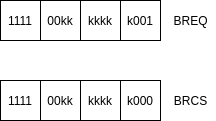
\includegraphics[width=150px]{images/6_Instruction_set/BREQ_BRCS_opcode.png}
    \end{figure}
    
    \item BRCC in confronto a BRCS ha opcode diverso (i primi 13 bit) ma gli ultimi 3 bit identici, appunto perché controllano lo stesso flag
    
    \begin{figure}[H]
        \centering
        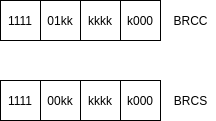
\includegraphics[width=150px]{images/6_Instruction_set/BRCC_BRCS_opcode.png}
    \end{figure}
    
    \item LDI ha 4 bit per indirizzare il registro destinatario, si assume il MSB come 1 quindi possiamo indirizzare i registri da 16 a 31, questo vale per tutte le istruzioni con operando immediato

    \begin{figure}[H]
        \centering
        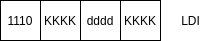
\includegraphics[width=150px]{images/6_Instruction_set/LDI_opcode.png}
    \end{figure}

\end{itemize}

Questo processore è a 8 bit tuttavia le istruzioni sono codificate su 16 bit.
Questo ci permette di avere molte più istruzioni normali e meno istruzioni che sforano andando sui 32 bit (alcuni esempi sono la CALL e la JMP che vogliono l'indirizzo per intero nell' istruzione).
Questa caratteristica porta ad avere una notevole \emph{code density} quindi nello stesso spazio ci sono molte più istruzioni che se fossero codificate su 32 bit.






\section{Funzionamento dell'assemblatore e aritmetica degli indirizzi}
Il software si scrive utilizzando un comune editor di testo, il codice sorgente non è nient' altro che testo, per trasformarlo in codice macchina comprensibile dal microcontrollore si deve utilizzare un programma chiamato \emph{assemblatore}.
Questo software si occupa di prendere il testo, leggerlo, trasformare il sorgente in codice macchina e costruire un file \emph{binario} pronto per essere scritto sulla memoria FLASH del SoC.

\subsection{Location counter}
Per eseguire la traduzione l'assemblatore ha la necessità di conoscere l' indirizzo di ogni istruzione, per fare ciò una variabile chiamata \emph{location\_counter} viene inizializzata a zero e man mano che le istruzioni del codice sorgente vengono elaborate viene incrementato (di 1 o 2 in base alla lunghezza dell'istruzione costruita).
\begin{verbatim}
    LDI r9, 47      # address: 0, size: 1
    ADIW r10, 810   # address: 1, size: 2
    MOV r0, r3      # address: 3, size: 1
\end{verbatim}

Attraverso alcune direttive all'assemblatore il location\_counter si può modificare, questo è spesso utilizzato per lasciare buchi nella flash.

\subsection{Simboli}
Un simbolo è una stringa di testo usata come identificatore per un valore.
Si possono usare lettere e numeri (non come primo carattere), sono case-insensitive, gli underscore (\_) sono ammessi.
L'assemblatore associa a ciascun simbolo un valore a 16 bit, si costruisce una tabella man mano che si va avanti e si incontrano dichiarazioni di simboli.
Ci sono due metodi per dichiarare un simbolo:
\begin{itemize}
    \item direttive .EQU e .DEF:
    \begin{verbatim}
        .EQU FOO=0x3900
        .DEF BAR=0x03A0
    \end{verbatim}
    entrambe queste direttive associano il valore a destra dell' uguale alla stringa a sinistra dell' uguale
    
    \item etichette:
    \begin{verbatim}
        QUI: <istruzione>
    \end{verbatim}
    si associa l' indirizzo dell' istruzione (il valore del location\_counter) all' etichetta specificata
\end{itemize}

\subsubsection{Etichette nei salti}
Le etichette possono essere utilizzate all' interno dei salti per non dover calcolare manualmente gli offset e gli indirizzi:
\begin{verbatim}
    RESET:
        RJMP START
    
    START:
        LDI r16, 0x5f
        LDI r17, 0x08
\end{verbatim}
Il codice di un ciclo di ritardo potrebbe quindi essere scritto:
\begin{verbatim}
        LDI r16, 100
    CICLO:
        DEC r16
        BRNE CICLO
\end{verbatim}

\subsubsection{Etichette nelle espressioni}
Le etichette possono essere utilizzate, come placeholder dei loro valori, all' interno delle espressioni, purché se ne conosca il valore a tempo di assemblaggio.








\section{Istruzione LPM}
L' istruzione LPM (Load Program Memory) permette di leggere dati dalla flash e porle all' interno di un registro.
Questo può tornare utile perché all' interno della flash poniamo i valori costanti come le stringhe, le lookup table, ecc.
Legge 1 byte per volta quindi non una riga intera!
Per indirizzare una cella si usa il registro $Z$ ma la sintassi dell' indirizzo è particolare:
\begin{figure}[H]
    \centering
    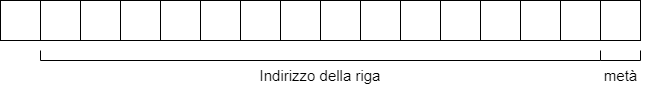
\includegraphics[width=300px]{images/8_LPM/LPM_sintassi.png}
\end{figure}
sui 16 bit del registro $Z$ i 14 bit centrali contengono l'indirizzo della riga da leggere, il bit meno significativo contiene un bit che indica:
\begin{itemize}
    \item 0: metà inferiore della riga
    \item 1: metà superiore della riga
\end{itemize}
il bit più significativo invece non è usato.

Supponiamo dunque di voler leggere alla cella con etichetta STRINGA:
\begin{verbatim}
    LDI ZL, low(STRINGA*2)
    LDI ZH, high(STRINGA*2)
    LPM
\end{verbatim}
le "funzioni" \emph{low} e \emph{high} si usano per dire all'assemblatore di prendere la parte alta o la parte bassa di un valore a 16 bit.
Inoltre l'istruzione ha un indirizzamento implicito, infatti non diamo nessun parametro, legge l'indirizzo da $Z$ e pone il byte letto in r0, in fine incrementa $Z$ di 1, in questo modo ora punterà al byte più significativo della riga.
Di fatto la sintassi di LPM è come se fosse:
\begin{verbatim}
    LPM r0, Z+
\end{verbatim}

Questo auto-incremento è utile per l'utilizzo nei loop, usati spesso per leggere stringhe dalla FLASH, a tal proposito una stringa nella FLASH si usa terminarla con un byte nullo, quindi per leggerla si potrebbe usare:
\begin{verbatim}
        LDI ZL, low(STRINGA*2)
        LDI ZH, high(STRINGA*2)
    corpo_lettura:
        LPM
        TST r0
        BREQ fuori
            ; uso del carattere in r0
        RJMP corpo_lettura
    fuori:
\end{verbatim}













\section{Stack}
E' una struttura dati costruita in SRAM utilizzata dal processore ma anche dal programmatore.
E' una struttura di tipo LIFO (Last-In-First-Out):
\begin{figure}[H]
    \centering
    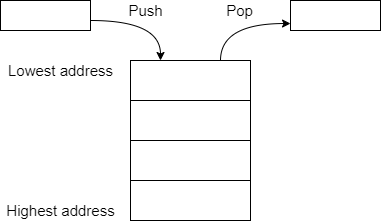
\includegraphics[width=250px]{images/9_Stack/stack.png}
\end{figure}

\subsection{Sub-routine}
E' utilizzata automaticamente dal processore per la chiamata alle sub-routine: supponiamo di avere un pezzo di codice che si occupa di calcolare la radice quadrata alla label RADQ, supponiamo di accedervi tramite l' istruzione JMP:
\begin{verbatim}
    LDI r0, low(900)
    LDI r1, high(900)
        # carico il valore di cui calcolare la sqrt
    JMP radq
        # salto alla procedura
\end{verbatim}
per ritornare al punto in cui ho chiamato la procedura mi servirebbe porre alla fine della procedura un' altra istruzione di salto:
\begin{verbatim}
    JMP foo
\end{verbatim}
Se ora volessi riutilizzare la procedura in un altro punto del codice non potrei perché alla fine di essa mi salterebbe sempre alla fine della prima chiamata!
Per risolvere questo problema sono state introdotte due istruzioni per gestire l' aggancio alle sub-routine:
\begin{itemize}
    \item RCALL radq: salva sullo stack il contenuto del registro PC + 1, sostituisce a PC il valore PC + k + 1.
    E' un salto relativo quindi nell' istruzione ci va un offset, tuttavia a noi basta specificare un' etichetta, l' offset lo calcolerà l'assemblatore per noi.
    Essendo un salto relativo può succedere che non funzioni se l' indirizzo al quale vogliamo andare è troppo lontano.

    \item ICALL radq: salva sullo stack il contenuto del registro PC + 1, sostituisce al registro PC il contenuto del registro Z.
    E' un salto assoluto quindi possiamo specificare l'intero indirizzo al quale vogliamo andare.

    \item CALL radq: salto assoluto che mette l' indirizzo al quale saltare direttamente nell' istruzione.

    \item RET: posto alla fine della procedura riprende il valore salvato sullo stack e lo mette in PC in modo da poter tornare al chiamante.
\end{itemize}
Per eseguire questo genere di operazioni potrebbe bastare salvare il valore in un registro?
No perché non sarebbe possibile innestare varie chiamate l'una dentro l'altra!

\subsection{Utilizzo diretto}
All' avvio del microcontrollore lo stack non è abilitato, va fatto via codice.
Per fare ciò si ricorre a due periferiche: SPL, SPH (SP - Stack Pointer).
All' interno di queste periferiche si inserisce l'indirizzo di inizio dello stack e da quel momento il processore ha lo stack abilitato.

\begin{figure}[H]
    \centering
    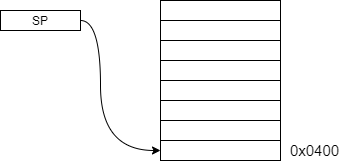
\includegraphics[width=250px]{images/9_Stack/SP.png}
\end{figure}

Possiamo interagire direttamente con lo stack attraverso due istruzioni:
\begin{itemize}
    \item PUSH rs: salva all' indirizzo correntemente puntato da SP il valore del registro passato e decrementa il valore di SP di 1 (la pila cresce verso indizzi più bassi)
    \item POP rd: decrementa il valore di SP e posiziona nel registro passato il valore puntato da SP
    (la pila decresce verso indirizzi più alti)
\end{itemize}

Di solito allo stack si riserva la parte finale della SRAM, un esempio di inizializzazione sarebbe dunque:
\begin{verbatim}
    LDI r16, low(0x085F)
    LDI r17, high(0x085F)
    OUT 0x3D, r16
    OUT 0x3E, r17
\end{verbatim}

Usare gli indirizzi raw è abbastanza caotico, la ATMEL e quindi l'ambiente di sviluppo, mettono a disposizione delle etichette già esistenti per tutti quei valori utili all' interno della programmazione, possiamo pertanto utilizzarli:
\begin{verbatim}
    LDI r16, low(RAMEND)
    LDI r17, high(RAMEND)
    OUT SPL, r16
    OUT SPH, r17
\end{verbatim}

\subsubsection{Swap di due registri}
Un esempio di utilizzo è quello dello swap di due registri:
\begin{verbatim}
    PUSH r10
    MOV r0, r1
    POP r1
    
    
    PUSH r0
    PUSH r1
    POP r0
    POP r1
\end{verbatim}

\subsection{Leggere il valore di PC}
Se per qualche motivo dovesse essere importante leggere il valore di PC si può usare:
\begin{verbatim}
    RCALL 0
        # salva sullo stack PC + 1
        # cioè l'indirizzo della prossima istruzione
    POP r0
    POP r1
\end{verbatim}





\section{Altre strutture dell' assemblatore}
\subsection{Direttive}
Abbiamo detto che l' assemblatore si occupa di prendere il nostro codice assembly e produrre un file caricabile sulla flash del controllore, tuttavia non fa solo questo.
In particolare si occupa anche di gestire gli indirizzi attraverso le etichette e ci toglie il lavoro di fare i calcoli per i salti relativi.

Al suo interno ha 3 location\_counter:
\begin{itemize}
    \item CSEG: location\_counter della flash
    \item DSEG: location\_counter della SRAM
    \item ESEG: location\_counter della EEPROM
\end{itemize}
questi 3 contatori sono usati per mantenere gli indirizzi mentre si avanza con la traduzione, all' avvio partono tutti da 0 anche se DSEG a 0 è inutile in quanto lì non c'è SRAM ed all' avvio è attivo il contatore CSEG quindi di default siamo in una sezione codice.

Possiamo dare delle istruzioni all' assemblatore attraverso le \emph{direttive}, si usano per modificare i contatori, aggiungere informazioni utili e tanto altro.
Iniziano tutte con il . davanti.

\subsubsection{.BYTE}
Ci permette di creare della "variabili" cioè associare un nome mnemonico ad un indirizzo della SRAM.
\begin{verbatim}
    NOME_VARIABILE: .BYTE <dimensione>
\end{verbatim}
il nome viene specificato tramite una etichetta, successivamente la direttiva .BYTE alloca tanti byte quanti specificati nella dimensione.
\begin{verbatim}
    array10: .BYTE 10
    array20: .BYTE 10+10
\end{verbatim}
Dato che stiamo parlando della SRAM l' assemblatore usa il contatore DSEG per assegnare l' indirizzo, quindi lo incrementa.

\subsubsection{.DSEG, .CSEG, .ESEG}
Sono direttive che indicano all' assemblatore quale location counter usare come principale da quel momento in poi.
Di fatto usarne uno indica che si sta creando una nuova sezione in quel tipo di memoria.

\subsubsection{.DB}
Si usa per allocare costanti, quindi diamo un nome ad un valore scritto nella FLASH.
\begin{verbatim}
    NOME_COSTANTE: .DB <lista_di_valori>
\end{verbatim}
in base alla lunghezza della lista sceglie quanti byte utilizzare e quindi quanto lunga sarà questa struttura.
Essendo in FLASH alloca sempre un numero pari di byte per prendere tutta la riga.
Se specifichiamo un valore più grande di 255 esso verrà troncato ai primi 8 bit.
\begin{verbatim}
    consts: .DB 0, 255, 0b01010101, -128, 0xaa
    str:    .DB "asg!\0"
    char:   .DB 'c'
\end{verbatim}

\subsubsection{.DEF}
Si usa per dare un sinonimo ad un registro.
\begin{verbatim}
    .DEF Symbol=Register
\end{verbatim}

\subsubsection{.DEVICE}
Si usa per specificare per quale dispositivo si sta scrivendo il codice.
Questo è utile per far comprendere all' assemblatore quale subset di istruzioni sono accettabili.
Non è necessario usarlo, in tal caso però l' assemblatore userà tutte le istruzioni possibili quindi se una non è supportata dal microcontrollore non ci verrà detto.

\subsubsection{.DW}
Si usa per allocare costanti a 16 bit.
\begin{verbatim}
    NOME_COSTANTE: .DW <lista_di_valori>
\end{verbatim}
Anche in questo caso se la variabile è più di 16 bit verrà troncata.
\begin{verbatim}
    varlist: .DW 0, 0xffff, 0b1001100110011001, -32768, 65535
\end{verbatim}

\subsubsection{.EQU}
Definisce un simbolo con un valore.
\begin{verbatim}
    .EQU var1=3
    .EQU var2=var1*3
\end{verbatim}
Si possono usare tutte le espressioni costanti per indicare il valore.

\subsubsection{.EXIT}
Si usa per indicare la fine di un file, quando viene incontrata dall' assemblatore esso smette di processare il file corrente.
Non è obbligatorio usarla.

\subsubsection{.INCLUDE}
Include il file specificato nel punto in cui uso la direttiva.
In questo assembly, detto \emph{assoluto} non conviene separare il codice in troppi file per lavorare in gruppo, questo perché le etichette non possono ripetersi pertanto diverse persone a scrivere il codice significa più probabilità di commettere errori di questo tipo.
Gli assembly che permettono questa feature sono detti \emph{relativi}.

\subsubsection{.LIST}
Abilita la creazione del list file, cioè un file che contiene gli indirizzi delle singole istruzioni, il loro codice operativo assieme all' assembly.
Può tornare utile ai fini di debug.

\subsubsection{.LISTMAC}
Aggiunge le macro nel listfile.

\subsubsection{.MACRO}
Si usa per creare delle pseudoistruzioni cioè mnemonici che poi vengono sostituiti con altre operazioni.
\begin{verbatim}
    .MACRO NOME_MACRO
        <espanzione della macro>
    .ENDMACRO
\end{verbatim}
All' interno della espansione si possono usare i parametri usando la sintassi \verb{@n{ con $n$ il numero della posizione del parametro.
\begin{verbatim}
    .MACRO SUBI16
        subi @1, low(@0)
        sbci @2, high(@0)
    .ENDMACRO
\end{verbatim}
Per usare la macro non serve altro che scriverne il nome e specificare i parametri.
\begin{verbatim}
    .CSEG
    SUBI16 0x1234, r16, r17
    ; verrà tradotto con
    ; subi r16, low(0x1234)
    ; sbci r17, high(0x1234)
\end{verbatim}

Si consiglia di usare le macro per espansioni di poche istruzioni o pseudoistruzioni, se sono tante ed usate spesso conviene creare ed usare delle sub-routine.

\subsubsection{.ORG}
Altera a mano il location\_counter attivo in quel momento


\subsection{Funzioni}
Ci sono anche alcune funzioni che si possono applicare ai valori costanti, queste vengono calcolate dall' assemblatore che poi sostituisce le chiamate con i valori effettivi.

\subsubsection{LOW}
Applicata ad un numero restituisce gli 8 bit più bassi.

\subsubsection{HIGH}
Applicata ad un numero restituisce i bit dall'8 al 15.

\subsubsection{EXP2}
Applicata ad un numero restituisce la sua potenza di 2.

\subsubsection{LOG2}
Applicata ad un numero restituisce la parte intera del suo logaritmo in base 2.


\subsection{Operatori}
Abbiamo a disposizione tutti gli operatori del C per calcolare le espresioni costanti.
\begin{table}[H]
    \centering
    \begin{tabular}{c|c}
        Operatore & Significato \\
         ! & NOT logico \\
         $ \Tilde{} $ & NOT binario \\ 
         - & meno unario \\ 
         * & moltiplicazione \\ 
         / & divisione intera \\ 
         + & somma \\ 
         - & sottrazione \\ 
         $<<$ & shift a sinistra \\
         $>>$ & shift a destra \\
         $<$ & minore \\
         $<=$ & minore o uguale \\
         $>$ & maggiore \\
         $>=$ & maggiore o uguale \\
         == & controllo di uguaglianza \\
         != & controllo di diversità \\
         \& & AND bit a bit \\
         $\wedge$ & XOR bit a bit \\
         $|$ & OR bit a bit \\
         \&\& & AND logico \\
         $||$ & OR logico \\
    \end{tabular}
\end{table}




\section{Primo programma}
Vogliamo fare un programma che esegue la divisione tra un numero a 16 bit ed uno a 8 bit:
\begin{verbatim}
    .include "m32def.inc"   ; includiamo i simboli messi
                            ; a disposizione da ATMEL
    .equ dividendo=1000
    .equ divisore=150

    .org 0x2a               ; lascio spazio vuoto fino a 0x2a
    
    start:
        ldi r16, low(RAMEND)
        ldi r17, high(RAMEND)
        out SPL, r16
        out SPH, r17
        ; stack inizializzato
        
        ldi XL, low(dividendo)
        ldi XH, high(dividendo)
        ldi YL, low(divisore)
        clr YH
        
        rcall divb
    
    fine:
        rjmp fine
        ; program halt
    
    ; X:    dividendo
    ; YL:   divisore
    ; Z:    quoziente
    ; divisione attraverso sottrazioni successive
    divb:
        tst YL
        brne ok
        sec         ; setto il carry
                    ; per segnalare errore
        ret
    
    ok:
        clr ZH
        clr ZL
        clr r0
    
    test:
        cp XL, YL
        cpc XH, r0  ; se ho carry ho finito
        brcc avanti
        clc
        ret
    
    avanti:
        sub XL, YL
        sbc XH, r0
        adiw ZL, 1
        rjmp test
\end{verbatim}
Compilando il programma si ottengono:
\begin{itemize}
    \item .hex: codice da flashare ul uC
    \item .lss: listato del programma compilato
    \item .map: contiene i valori dei simboli, sono numeri rappresentati su 32 bit ma in realtà durante l' assemblaggio vengono troncati a 16
\end{itemize}

Si ricordi che il file ottenuto dall' assemblaggio va flashato sulla FLASH interna del uC, per fare ciò bisogna cancellare tutto il suo contenuto, questo non fa altro che settare ad 1 tutta la flash, dopodiché si scrivono gli 0.
Questo si fa perché le memorie flash permettono di passare un singolo bit da 1 a 0 ma non viceversa, per fare ciò si deve cancellare tutto quanto, resettare la flash, quindi in genere non si fa a runtime una scrittura in flash.
Inoltre le flash hanno un numero massimo di riscritture, in particolare l' ATmega32 garantisce fino a 10k scritture.



\section{Divisione efficiente}
L' algoritmo usato precedentemente non risulta molto efficiente e soprattutto non è in tempo costante.
Un algoritmo migliore sarebbe quello che si vede alle elementari: la divisione in colonna.
Supponiamo di dover dividere 19374 per 171:
\begin{itemize}
    \item si prendono le prime 3 cifre del dividendo: 193 e si controlla quante volte entri nel divisore 171, in questo caso entra 1 volta
    
    \item il quoziente ha come prima cifra 1

    \item sottraggo 171 a 193 ed ottengo il primo resto
    
    \item abbasso la prossima cifra e ripeto il controllo e l' aggiornamento
\end{itemize}
Abbiamo alcuni problemi nello scegliere quante cifre prendere, se ne prendo poche ottengo 0 come cifra, in realtà va bene in quanto mi fornisce uno 0 in testa che fa parte del quoziente.
Inoltre in binario ci viene ancora più semplice la fase di comparazione in quanto un numero può entrare nell' altro solo 0 o 1 volte e per saperlo ci basta vedere quale dei due valori risulta maggiore dell' altro.

Supponiamo dunque di voler eseguire una divisione a 16 bit completa: $\frac{p}{q}$
\begin{itemize}
    \item $p$ a 16 bit
    \item $q$ a 16 bit
    \item $k$ quoziente può essere al massimo $\frac{65535}{1} = 65535$ che sta su 16 bit
\end{itemize}

Pongo il dividendo in due registri e lo estendo su 32 bit, per questo numero facciamo una estensione virtuale, nel senso che non usiamo registri per mantenere in memoria gli zeri più significativi.
Il divisore invece lo poniamo nella parte alta di 4 registri, quindi anche lui rappresentato su 32 bit.
La situazione iniziale deve quindi essere:
\begin{figure}[H]
    \centering
    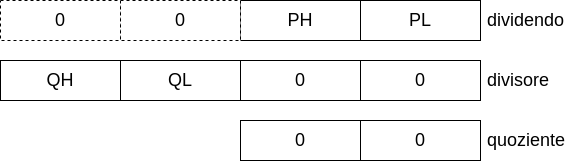
\includegraphics[width=250px]{images/12_Divisione_efficiente/divisione_fast.png}
\end{figure}

Ad ogni iterazione devo quindi vedere se $P > Q$, in tal caso ottengo 1, altrimenti 0:
\begin{itemize}
    \item se ottengo 1 sottraggo
    \item se ottengo 0 non faccio niente
\end{itemize}
alla fine shifto a destra Q.
Per collezionare le singole cifre le inserisco da destra all' interno del quoziente poi shifto a sinistra per farle andare al loro posto.
Si noti che la parte alta di P contiene degli zeri, quindi per i primi elementi il controllo si limita a vedere se la parte alta di Q è diversa da 0, per la parte bassa invece occorre un vera comparazione.
Dopo un po' di giri P e Q saranno allineati e quindi inizierò ad ottenere le vere cifre del quoziente.

L' algoritmo viene iterato per 16 volte, per non sprecare un registro inserisco un bit ad 1 come primo bit del quoziente, quando lo vedo comparire nel carry dopo gli shift so che ho fatto tutte le iterazioni necessarie.

Mappiamo i seguenti registri:
\begin{figure}[H]
    \centering
    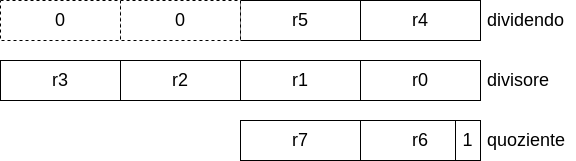
\includegraphics[width=250px]{images/12_Divisione_efficiente/divisione_fast_registri.png}
\end{figure}

\begin{verbatim}
    ; PARAMS
    ; r3:r2 divisore
    ; r5:r4 dividendo

    ; RETURN
    ; r5:r4 resto
    ; r7:r6 quoziente

    div16:
        ; controllo che non mi sia stato
        ; chiesto di dividere per 0
        mov r8, r2
        or r8, r3
        brne nodiv0

        ; in tal caso setto il carry come errore
        ; ed esco
        sec
        ret

        ; eseguo la vera divisione
    nodiv0:
        ; configuro i registri
        clr r0
        clr r1
        clr r6
        inc r6  ; inserisco 1 come LSB
        clr r7
        clr r8
        
    divstart:
        ; shift del divisore
        lsr r3  ; LSB va in carry
        ror r2  ; il carry va in MSB, LSB va in carry
        ror r1  ; il carry va in MSB, LSB va in carry
        ror r0  ; il carry va in MSB, LSB va in carry
        
        tst r3
        brne nosub
            ; se è diverso da 0 non devo sottrarre
        tst r2
        brne nosub
            ; se è diverso da 0 non devo sottrarre

        cp r5,r1
        brcs nosub
            ; r5 < r1 ho 0 e non devo sottrarre
        brne oksub
            ; r5 > r1 ho 1 e devo sottrarre 
            ; r5 == r1 devo controllare l'ultimo byte
        cp r4,r0
        brcs nosub
            ; r4 < r0 ho 0 e non devo sottrarre
            ; r4 >= r0 ho 1 e devo sottrarre
        
    oksub:
        ; eseguo la sottrazione
        sub r4,r0
        sbc r5,r1
        sec         ; setto il carry per inserire 1
        rjmp div1
        
    nosub:
        clc         ; pulisco il carry per inserire 0
        
    div1:
        rol r6
        rol r7
        brcc divstart
            ; se carry = 1 ho finito le iterazioni
        
    divfine:
        clc     ; divisionre corretta quindi carry = 0
        ret
\end{verbatim}


\section{Esercitazione 1}

\subsection{Radice quadrata con metodo di Newton}
Calcolare la radice quadrata di un numero a 16 bit:
$$ k = \sqrt{a} $$
tramite il metodo iterativo di Newton.

Se abbiamo $a$ a 16 bit la sua radice quadrata $k$ sta sempre su 8 bit.
Usando il metodo di Newton possiamo approssimare le soluzioni di $f(x) = 0$, nel nostro caso abbiamo $x^2 - a = 0$, in particolare a noi servono solo le soluzioni positive.
Il metodo di Newton prevede che si parta da un punto casuale, si tracci la tangete della funzione per quella coordinata $x$, si trovi l' intersezione con l' asse delle $x$ e si usi quel punto come nuova approssimazione per reiterare il processo.
\begin{figure}[H]
    \centering
    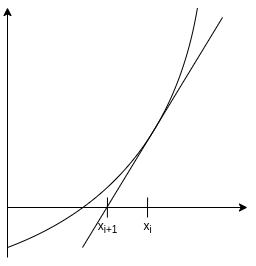
\includegraphics[width=220px]{images/13_Esercitazione_1/metodo_di_newton.png}
\end{figure}

Data la funzione $f(x) = x^2 - a$, abbiamo come derivata $\frac{\partial f}{\partial x} = 2x$, per tracciare la tangente nel punto $P_i(x_i, f(x_i)) = (x_i, x_i^2-a)$ dobbiamo risolvere:
$$ y - y_p = m(x - x_p) $$
Si ricordi che $m = \frac{\partial f}{\partial x}(x_i) = 2x_i$ quindi:
$$ y = 2x_i(x-x_i) + x_i^2 - a $$
$$ y = 2xx_i - x_i^2 - a $$
ci interessa l' intersezione con l'asse delle $x$ quindi quando $y=0$:
$$ 2xx_i - x_i^2 - a = 0 $$
$$ x_{i+1} = x = \frac{x_i^2 + a}{2x_i} $$
Dobbiamo eseguire una moltiplicazione, per il quadrato, una somma ed una divisione, possiamo arrangiarla diversamente:
$$ \frac{1}{2} \left( \frac{a + x_i^2}{x_i} \right) = \frac{1}{2} \left( \frac{a}{x_i} + x_i \right) $$
In questa formulazione ci bastano una divisione, una somma ed uno shift a destra.

Ci serve inoltre un punto per iniziare la nostra iterazione, per convergere in maniera veloce per questa funzione conviene scegliere un punto iniziale maggiore del valore effettivo, quindi dato che vale $a > \sqrt{a}$ se $a \neq 0, a \neq 1$, usiamo $a$ stesso come prima approssimazione.

Proviamo per $a = 100$:
$$ x_0 = 100 \xrightarrow{} x_1 = \left\lfloor \frac{1}{2} \left( \frac{100}{100} + 100 \right) \right\rfloor = 50 $$
$$ x_1 = 50 \xrightarrow{} x_2 = \left\lfloor \frac{1}{2} \left( \frac{100}{50} + 50 \right) \right\rfloor = 26 $$
$$ x_2 = 26 \xrightarrow{} x_3 = \left\lfloor \frac{1}{2} \left( \frac{100}{26} + 26 \right) \right\rfloor = 14 $$
$$ x_3 = 14 \xrightarrow{} x_4 = \left\lfloor \frac{1}{2} \left( \frac{100}{14} + 14 \right) \right\rfloor = 10 $$
$$ x_4 = 10 \xrightarrow{} x_5 = \left\lfloor \frac{1}{2} \left( \frac{100}{10} + 10 \right) \right\rfloor = 10 $$
Come criterio di stop possiamo usare $x_i = x_i+1$, con 4 iterazioni ho finito!

Provimo per $a = 900$:
$$ x_0 = 900 \xrightarrow{} x_1 = \left\lfloor \frac{1}{2} \left( \frac{900}{900} + 900 \right) \right\rfloor = 450 $$
$$ x_1 = 450 \xrightarrow{} x_2 = \left\lfloor \frac{1}{2} \left( \frac{900}{450} + 450 \right) \right\rfloor = 226 $$
$$ x_2 = 226 \xrightarrow{} x_3 = \left\lfloor \frac{1}{2} \left( \frac{900}{226} + 226 \right) \right\rfloor = 114 $$
$$ x_3 = 114 \xrightarrow{} x_4 = \left\lfloor \frac{1}{2} \left( \frac{900}{114} + 114 \right) \right\rfloor = 60 $$
$$ x_4 = 60 \xrightarrow{} x_5 = \left\lfloor \frac{1}{2} \left( \frac{900}{60} + 60 \right) \right\rfloor = 37 $$
$$ x_5 = 37 \xrightarrow{} x_6 = \left\lfloor \frac{1}{2} \left( \frac{900}{37} + 37 \right) \right\rfloor = 30 $$
$$ x_6 = 30 \xrightarrow{} x_7 = \left\lfloor \frac{1}{2} \left( \frac{900}{30} + 30 \right) \right\rfloor = 30 $$
Con 6 iterazioni abbiamo finito!

Si noti tuttavi che se il radicando non è perfetto il risultato potrebbe oscillare:
$$ x_1 = 13 $$
$$ x_2 = 12 $$
$$ x_3 = 13 $$
$$ x_4 = 12 $$
quindi come condizione di uscita useremo: $ x_i = x_{i+1} \vee x_i = x_{i+2} $

Si noti che i casi in cui $a = 0, a = 1$ vanno gestiti separatamente in quanto non si possono risolvere con l'algoritmo di Newton.

\subsection{Crivello di Eratostene}
Implementare in assembly il crivello di Eratostene per la ricerca dei numeri primi.

Si elencano tutti i numeri da 1 ad $N$, tralaciamo 1 e partiamo da 2:
\begin{itemize}
    \item elimino tutti i suoi multipli in successione, dato che servono in successione posso continuare a sommare 2 finché non arrivo oltre $N$, non servono dunque le moltiplicazioni
    
    \item prendo il prossimo numeri non cancellato ed eseguo l' algoritmo a partire da lui
\end{itemize}

NB: cancellare significa inserire al posto di quel numero un valore convenzionalemnte associato a niente, ad esempio lo 0.

\begin{verbatim}
    TODO: immagini del crivello in azione
\end{verbatim}

Si prenda $N$a scelta ma \emph{maggiore} di 1000, usando numeri a 16 bit si consiglia di rappresentare ogni numero su 16 bit.

Il programma deve quindi:
\begin{itemize}
    \item svuotare la RAM
    \item inzializzarla inserendo i numeri da 2 ad $N$
    \item eseguire il crivello
    \item compattare tutti i numeri primi trovati
\end{itemize}






\section{Endianness ed allineamento}
\subsection{Endianness}
Supponiamo di avere:
\begin{verbatim}
    .DSEG
    TEMP: .BYTE 2
\end{verbatim}
se agli indirizzi bassi mettiamo la parte meno significativa:
\begin{verbatim}
    STS TEMP, ZL
    STS TEMP+1, ZH
\end{verbatim}
stiamo trattando il dato come \emph{little endian}.

Se agli indirizzi bassi mettiamo la parte più significativa:
\begin{verbatim}
    STS TEMP, ZH
    STS TEMP+1, ZL
\end{verbatim}
stiamo trattando il dato come \emph{big endian}.

La CPU AVR è intrinsecamente little endian, per esempio nella RCALL pusha prima PCH e poi PCL (guardando gli indirizzi compaiono in big endian ma in questo caso conta l' ordine con il quale si eseguono le istruzioni).
Alcune operazioni poi hanno una endianness intrinseca.

Anche a livello di bit esiste una endianness: se devo invia dei bit in sequenza da quali bit inizio? Dal più significativo o dal meno significativo?

\subsection{Allineamento}
Alcune CPU come ARM hanno il bus dati a 32 bit ed ogni singola cella, byte, ha un proprio indirizzo.
Fisicamente trasferisco 4 byte per volta quindi legge 4 byte ma poi trasferisce nei registri solo le parti interessate.
Se voglio leggere un intero a 32 bit:
\begin{itemize}
    \item se leggo da un multiplo di 4 leggo tutta la riga
    \item se leggo da un indirizzo arbitrario c'è un probema di allineamento:
    \begin{verbatim}
        MOV r1, 0x000A
    \end{verbatim}
    \begin{figure}[H]
        \centering
        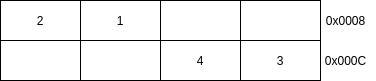
\includegraphics[width=200px]{images/14_Endianness_e_allineamento/accesso_disallineato.png}
    \end{figure}
    per leggere il valore dovrei leggere le due righe e poi ri-assemblare il valore ottenuto per metterlo nel registro.
    
    Gli accessi non allineati sono molto meno efficienti!
\end{itemize}

Altre CPU come AVR invece danno un indirizzo alla riga, 2 byte, non alla singola cella.
Inoltre le occasioni per eseguire accessi non allineati sono molto poche dato che la SRAM ha accessi a byte.

ARM si rifiuta di fare JMP ad indirizzi non multipli di 4.
Intel invece ha gli accessi allineati facoltativi per retrocompatibilità.
Altri processori se si fa un accesso non allineato leggono male senza dare errori.

Ci sono alcune direttive per imporre l' allineamento:
\begin{verbatim}
    .ALIGN(2)
        ; allinea il location_counter a 2
\end{verbatim}
tuttavia spesso conviene evitare di usarle in quanto portano a spreco di memoria utile quando è poca.
Ad esempio nelle strutture del C, che tende ad inserire tutto allineato il più possibile ci sono molti spazi vuoti di \emph{padding}, spesso conviene richiedere al compilatore la soppressione del padding per risparmiare spazio.


\section{Esercitazione 2}
Scrivere un programma in assembly che calcoli il fattoriale su 16 bit di un numero e poi lo converta in ASCII in modo da rappresentarlo nel dump di memoria del microcontrollore.
Organizzare il codice in sottoprocedure e la subprocedure per il calcolo del fattoriale deve essere ricorsiva.


\chapter{Gestione delle periferiche}
\section{Interrupt}
E' un meccanismo genericamente implementato per gestire le periferiche, i dati arrivano in maniera aleatoria quindi stando a quanto conosciamo adesso dovremmo controllare periodicamente lo stato delle periferiche alla ricerca di un nuovo valore, questo è detto \emph{polling}.
Tuttavia è poco efficiente in quanto il tempo impiegato a controllare è tempo sprecato che potrei passare a fare altro quindi conviene solo su flussi di dati abbondanti in cui il \emph{success rate} delle interrogazioni è alto.
Inoltre se passa troppo tempo tra un controllo e l' altro i dati potrebbero essere troppo vecchi da utilizzare. 
Sarebbe bello essere notificati dalla periferica qualora avesse un nuovo valore per noi.

Per fare ciò ci vengono in aiuto le interruzioni (\emph{interrupts}), il nostro ATMega32 ha 3 sorgenti di interruzioni esterne: quando una periferica ha un valore lo segnala tramite un trigger specifico, al trigger il uC salta direttamente ad una parte del codice predisposta alla gestione di quel trigger.
Alla fine di questo codice, detto \emph{handler}, vi è una ret che permette di tornare al codice interrotto e riprendere l'esecuzione.

\begin{figure}[H]
    \centering
    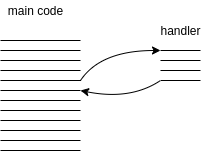
\includegraphics[width=150px]{images/15_Interrupt/interrupt_example.png}
\end{figure}

\subsection{Funzionamento}
Ognuno degli interrupt ha:
\begin{itemize}
    \item un flag di abilitazione: ENABLE bit
    \item un flag che indica se c'è un interrupt \emph{pendente}: FLAG bit
\end{itemize}
Quando arriva un evento viene settato il bit FLAG e se anche il bit ENABLE è attivato alla fine della prossima fase di esecuzione verrà eseguito il salto all' handler.
Quando viene effettuato il salto all' handler si disabilita anche il FLAG bit in quanto non si deve risaltare nuovamente all' handler finché non arriva un altro evento.

In fine c'è anche un bit generico per disabilitare tutte le interruzioni assieme, questo è il bit I all' interno dello SREG, se è disabilitato qualsiasi interruzione è disabilitata.
Questo flag viene disabilitato di default all' ingresso in un handler.

Gli indirizzi ai quali saltare in base all' interruzione sono hard-coded nel uC e sono quindi fissi.
Questi indirizzi coincidono con gli indirizzi delle righe della \emph{interrupt vector table} una tabella che va dall' indirizzo 0x0000 all' indirizzo 0x002a della FLASH. Abbiamo quindi 20 interruzioni diverse.

\begin{figure}[H]
    \centering
    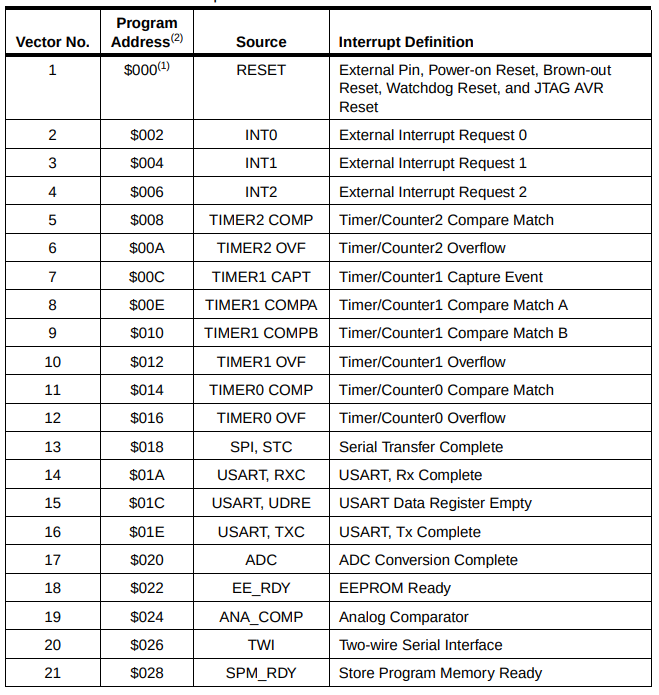
\includegraphics[width=300px]{images/15_Interrupt/interrupt_vector_table.png}
\end{figure}

Il codice delle interruzioni è direttamente in questa tabella, abbiamo quindi 32 bit di spazio per handler, abbastanza da poterci inserire una RJMP (1 riga) o una JMP (2 righe) ad una subroutine più grande.

\begin{figure}[H]
    \centering
    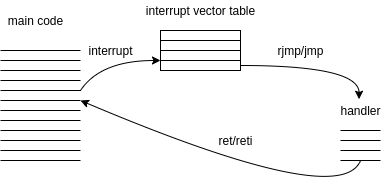
\includegraphics[width=250px]{images/15_Interrupt/interrupt_handler_with_table.png}
\end{figure}

NB: all' avvio le interruzioni sono tutte disabilitate, sia i singoli ENABLE bit che il flag I, questo perché bisogna prima di tutto abilitare lo stack altrimenti l' handler non potrà ritornare al codice.

NB: si noti che gli interrupt non salvano i registri ne i flag quando si entra, quindi bisogna creare procedure che non modifichino i registri ne i flag altrimenti il codice principale potrà fornire risultati sbagliati:
\begin{verbatim}
    push r0
    in r0, SREG
    push r0
        ; salva i flag sullo stack
    
    pop r0
    out SREG, r0
    pop r0
        ; ripristino i flag
\end{verbatim}

\subsubsection{Interrupt nidificati}
Abbiamo detto che all' entrata nell' handler il bit I viene disabilitato, questo fa si che tutte le interrzioni siano abilitate globalmente.
Se volessimo dare la possibilità di avere interrupt annidati dobbiamo abilitare il bit I a mano all' entrata dell' handler.

Bisogna fare molta attenzione a questi casi in quanto se gli interrupt avvengono troppo di frequente potrei non riuscire a finire quelli già iniziati e saturare lo stack di indirizzi di ritorno, inoltre il codice principale sarebbe eternamente bloccato!
\begin{verbatim}
    cli
        ; pone I a 0: disabilita le interruzioni
        
    sti
        ; pone I a 1: abilita le interruzioni
\end{verbatim}

Se invece all' interno di un handler ho le interruzioni disabilitate ma arriva un altro trigger da qualche perifericha il bit FLAG viene abilitato e vi rimane finché non decido di riabilitare le interruzioni e quindi servirlo.
In questo caso si parla di interrupt pendente.
Si noti che se ci sono più interrupt pendenti dello stesso tipo ne verrà gestito solo uno in quanto il flag non permette di contare quante volte è avvenuto l' evento.

Se invece ci sono più interrupt pendenti di tipo diverso quello che viene gestito prima è quello con indirizzo nella interrupt vector table minore.

\subsubsection{Ritorno dall' handler}
Per ritornare da un handler possiamo usare:
\begin{itemize}
    \item RET: semplicemente torna al chiamante prendendo l' indirizzo dallo stack
    \item RETI: oltre a tornare al chiamante abilita anche il flag I
\end{itemize}

\subsection{Interruzioni esterne}
Il package del uC ha 3 pin nominati INT0, INT1, INT2 che sono programmabili per recepire variazioni del segnale e lanciare interruzioni.
INT0 e INT1 sono praticamente identici mentre INT2 è più limitato nelle funzionalità in quanto introdotto successivamente.

\subsubsection{INT0 e INT1}
Possono essere programmati per lanciare un handler:
\begin{itemize}
    \item sul fronte di salita - \emph{rising edge}:
        \begin{figure}[H]
            \centering
            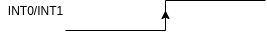
\includegraphics[width=150px]{images/15_Interrupt/rising_edge.png}
        \end{figure}
        
    \item sul fronte di discesa - \emph{fallnig edge}:
        \begin{figure}[H]
            \centering
            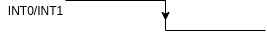
\includegraphics[width=150px]{images/15_Interrupt/falling_edge.png}
        \end{figure}

    \item su qualsiasi fronte:
        \begin{figure}[H]
            \centering
            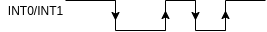
\includegraphics[width=150px]{images/15_Interrupt/each_edge.png}
        \end{figure}

    \item sul livello basso:
        \begin{figure}[H]
            \centering
            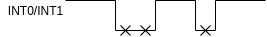
\includegraphics[width=150px]{images/15_Interrupt/low_level.png}
        \end{figure}
        Questa modalità è particolarmente utile per eseguire un multiplexing degli interrupt esterni: supponiamo che 3 interrupt non ci bastino, posso configurare la detection sul livello basso ed usare questo circuito:
        \begin{figure}[H]
            \centering
            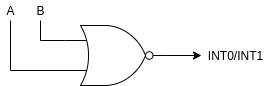
\includegraphics[width=150px]{images/15_Interrupt/interrupt_multiplexing.png}
        \end{figure}
        Ho quindi due sorgenti di interruzioni A e B che vanno in una porta NOR e finché almeno uno dei 2 è alto l' uscita  della porta sarà bassa.
        Avendo la rilevazione sul livello logico 0 detecto questa condizione, salto all' handler disabilitando le interruzioni, interrogo le periferiche per vedere quella che mi ha chiesto di essere gestita, la gestisco e porrà a 0 la sua richiesta. Pulisco infine il FLAG bit a mano e ritorno dall' handler.
        Se anche l' altra periferica vuole essere gestita allora subito dopo aver pulito il FLAG bit esso verrà nuovamente riattivato e quindi partirò gestendo la seconda interruzione.
\end{itemize}

Per abilitare uno dei due interrupt si deve prima configurare la modalità di utilizzo all' interno del registro MCUCR:
\begin{figure}[H]
    \centering
    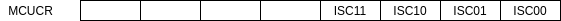
\includegraphics[width=320px]{images/15_Interrupt/MCUCR.png}
\end{figure}
\begin{itemize}
    \item ISC01:ISC00: indicano la modalità di funzionamento dell' interrupt 0
    \item ISC11:ISC10: indicano la modalità di funzionamento dell' interrupt 1
\end{itemize}
le modalità sono codificate:
\begin{table}[ht!]
    \centering
    \begin{tabular}{c|c|l}
        ISCX1 & ISCX0 & modalità \\
        \hline
        0 & 0 & livello basso \\
        0 & 1 & qualsiasi variazione \\
        1 & 0 & falling edge \\
        1 & 1 & rising edge \\
    \end{tabular}
\end{table}

Es: INT1 sul falling edge e INT0 su qualsiasi variazione:
\begin{verbatim}
    ldi r16, (1 << ISC11)|(1 << ISC00)
    out MCUCR, r16
        ; NO! sovrascrivo anche i bit che
        ; magari non voglio toccare
    
    in r16, MCUCR
    ori r16, (1 << ISC11)|(1 << ISC00)
    out MCUCR, r16
        ; cambio solo i bit necessari
\end{verbatim}

\subsubsection{INT2}
Ha solo un bit di controllo localizzato in MCUCSR:
\begin{figure}[H]
    \centering
    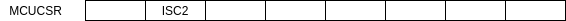
\includegraphics[width=320px]{images/15_Interrupt/MCUCSR.png}
\end{figure}
le modalità sono codificate:
\begin{table}[ht!]
    \centering
    \begin{tabular}{c|l}
        ISC2 & modalità \\
        \hline
        0 & falling edge \\
        1 & rising edge \\
    \end{tabular}
\end{table}

\subsubsection{Abilitazione interrupt}
Una volta configurata la modalità di funzionamento si devono abilitare i singoli interrupt, per fare ciò abbiamo 3 flag nel registro GICR:
\begin{figure}[H]
    \centering
    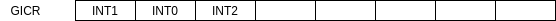
\includegraphics[width=320px]{images/15_Interrupt/GICR.png}
\end{figure}
posto 1 in uno degli slot abilita l'interrupt corrispondente.

\subsubsection{Bit di interrupt pendente}
I bit di interrupt pendente sono nel registro GIFR:
\begin{figure}[H]
    \centering
    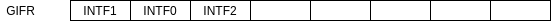
\includegraphics[width=320px]{images/15_Interrupt/GIFR.png}
\end{figure}
per pulirli bisogna scriverci 1 mentre può settarli solo l' hardware.

\subsection{Esempio di programma}
\begin{verbatim}
    .include "m32def.h"
    reset:
        rjmp start
    
    .org 0x0001
    int0_vect:
        rjmp int0_handler
    
    .org 0x002a
    start:
            ; abilitiamo lo stack che ci 
            ; serve per le interruzioni
        ldi r16, low(RAMEND)
        ldi r17, high(RAMEND)
        out spl, r16
        out sph, r17
        
            ; impostiamo interrupt INT0
            ; su fronte di salita
        in r16, MCUCR
        ori r16, (1 << ISC01)|(1 << ISC00)
        out MCUCR, r16
            ; abilitiamo INT0
        in r16, GICR
        ori r16, (1 << INT0)
        out GICR, r16
            ; abilito le interruzioni
            sei
        
        ; yadda-yadda
        
    end:
        rjmp end
    
    
    int0_handler:
        ; codice dell' interrupt
        reti
\end{verbatim}

\subsection{Sezione critica}
Supponiamo di avere il segunte codice:
\begin{verbatim}
    add yl, xl
    adc yh, xh
\end{verbatim}
se una interruzione avviene tra la prima e la seconda potrei perdere il carry bit.
Questa è una sezione critica che quindi va eseguita in maniera \emph{atomica}.
Un codice più sicuro sarebbe ad esempio:
\begin{verbatim}
    cli         ; disabilito le interruzioni
    add yl, xl
    adc yh, xh
    sei         ; abilito le interruzioni
\end{verbatim}
l' interrupt è ritardato di qualche ciclo di clock, se la sezione critica è molto piccola va bene usare questo approccio.

Tuttavia c' è un problema:
\begin{itemize}
    \item se all' inizio della sezione critica $I=1$ allora l' uscita è coerente
    \item se all' inizio della sezione critica $I=0$ allora alla fine abbiamo attivato le interruzioni, probabilmente senza volerlo
\end{itemize}
una soluzione più generica è pertanto:
\begin{verbatim}
    in r0, SREG
    cli
        ; salvo i flag e disabilito le interruzioni
    add yl, xl
    adc yh, xh
    out SREG, r0
        ; rimetto i flag al loro posto
\end{verbatim}

Se si vuole essere ancora più raffinati possiamo usare delle macro:
\begin{verbatim}
    .macro save_irq
        in r0, SREG
        cli
    .endmacro
    
    .macro restore_irq
        out SREG, r0
    .endmacro
    
    save_irq
    add yl, xl
    adc yh, xh
    restore_irq
\end{verbatim}

Un' altra opzione è quella di creare handler che non modifichino flag e registri, ma questa soluzione non è universale in quanto a volte bisogna eseguire operazioni con un timing particolare quindi oltre al contenuto dei flag e registri importa anche il numero di cicli di clock impiegati tra le istruzioni.
\section{Sleep mode e reset}
\subsection{Sleep mode}
Per risparmiare energia posso disabilitare alcune componenti interne del chip attraverso il registro MCUCR:
\begin{figure}[H]
    \centering
    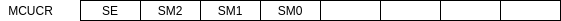
\includegraphics[width=320px]{images/16_Sleep_mode/MCUCR.png}
\end{figure}
Per andare in sleep mode si deve scrivere 1 nel bit SE del registro MCUCR e poi eseguire l'istruzione sleep:
\begin{verbatim}
    in r16, MCUCR
    ori r16, (1 << SE)
    out MCUCR, r16
    sleep
\end{verbatim}
Per risvegliarsi c' è bisogno di un interrupt.0
Abbiamo a disposizione 6 modalità diverse di sleep mode:
\begin{table}[H]
    \centering
    \begin{tabular}{p{0.05\linewidth} p{0.05\linewidth} p{0.05\linewidth} | p{0.7\linewidth}}
        SM2 & SM1 & SM0 & Descrizione \\
        \hline
        0 & 0 & 0 & Idle: tutto è attivo tranne la CPU, è comodo per bloccare l' esecuzione del codice in maniera temporanea. Si risparmia poco ma ci si sveglia molto velocemente \\
        \hline
        0 & 0 & 1 & ADC noise reduction: disabilita la CPU e ed alcune periferiche, si usa per diminuire il rumore durante la misurazione di un valore analogico attraverso l' ADC. Visto il grande utilizzo in questo senso: se l' ADC è abilitato quando si entra in questa modalità parte direttamente una misurazione \\
        \hline
        0 & 1 & 0 & Power down: spegne l' oscillatore esterno disabilitando tutti i clock generati \\
        \hline
        0 & 1 & 1 & Power save: blocca tutti i clock tranne $clk_{ASY}$ mantentendo in uso difatti solo i moduli asincroni \\
        \hline
        1 & 0 & 0 & Reserved \\
        \hline
        1 & 0 & 1 & Reserved \\
        \hline
        1 & 1 & 0 & Standby: identico al power-down ma l' oscillatore è tenuto attivo \\
        \hline
        1 & 1 & 1 & Extended standby: identico al power-save ma l' oscillatore è tenuto attivo \\
    \end{tabular}
\end{table}
Per maggiori informazioni sulle condizioni secondarie per attivare i vari stati fare riferimento al datasheet.


\subsection{Reset}
E' un evento che re-inizializza tutto il sistema e fa ripartire l' esecuzione dall' indirizzo 0x0000.
Può avvenire per vari motivi:
\begin{itemize}
    \item Power-on Reset: quando do l' alimentazione o quando la tensione di alimentazione scende oltre la soglia di Power-on
    \item External Reset: quando si pone il livello logico basso sul pin $\overline{RESET}$:
    \begin{figure}[H]
        \centering
        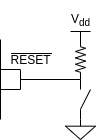
\includegraphics[width=75px]{images/16_Sleep_mode/reset_push_button.png}
    \end{figure}
    NB: a volte anche con un condensatore in parallelo al resistore.
    
    \item Watchdog Reset: è una periferica che periodicamente va contattata, se non lo si fa dopo un po' di tempo si ha un reset
    \item Brown-out Reset: quando la tensione scende un po' ma non va completamente a 0.
    In questi casi la CPU può commettere degli errori quindi un circuito analogico controlla la tensione e quando accade si ha un reset
    \item JTAG AVR Reset: reset inviato tramite una connessione JTAG
\end{itemize}

All' avvio del uC possiamo sapere quale sia stata la ragione del reset leggendo il registro MCUCSR:
\begin{figure}[H]
    \centering
    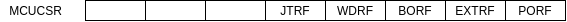
\includegraphics[width=320px]{images/16_Sleep_mode/MCUCSR.png}
\end{figure}
\begin{itemize}
    \item JTRF: JTAG reset
    \item WDRF: watchdog reset
    \item BORF: Brown-out reset
    \item EXTRF: external reset
    \item PORF: power-on reset
\end{itemize}

\section{Lock bits e clock}
Il clock usato dal uC in genere è esterno, ma il modello che stiamo analizzando ha al suo interno varie sorgenti di clock che possono essere utilizzate se non si vuole usare una fonte esterna.
Le tensioni di operatività sono:
\begin{itemize}
    \item 2.7 - 3.6V per ATMega32L (3.3V $\pm$ 10\%)
    \item 4.5 - 5.5V per ATMega32 (5V $\pm$ 10\%)
\end{itemize}
quindi il clock deve essere un' onda quadra che vada da 0V a Vdd con duty cycle del 50\%.
Per programmare il clock interno si deve ricorrere ai \emph{fuse} interni.

Il concetto di fuse (fusibile) era inizialmente utilizzato all' interno delle PROM, ogni singola cella era un fusibile, in fase di programmazione si faceva saltare o meno tramite apposite tensioni, questo metodo tuttavia non era molto reliable in quanto i microcrateri causati da queste detonazioni potevano richiudersi grazie ai detriti e quindi riprendere a condurre.
In seguito si è passati agli antifusibili cioè dei condensatori che di norma non conducono, quando gli si fa passare una corrente adeguata invece il dielettrico diventa una giunzione permanente.

In fine all' interno del uC vi è un' altra memoria flash a parte, detta \emph{lockbits}, che contiene dei bit utilizzati per la configurazione dell' hardware.

\subsection{Lock bits}

\subsubsection{Lock bit byte}
Sono bit usati per impedire la lettura della flash e quindi dumpare il firmware contenuto nel uC, ce n'è uno anche per impedire la riprogrammazione.

\subsubsection{Bit clock option}
E' il quarto bit del fuse high byte e si usa per indicare quale modalità operativa deve usare l' oscillatore amplificatore.

\subsubsection{Clock select}
Sono i bit 3, 2, 1, 0 del fuse low byte e si usano per indicare quale sorgente di clock il uC deve usare.

\subsubsection{Start-up time}
Sono i bit 5, 4 del fuse low byte, sono usati per indicare lo startup time del clock. 

\subsubsection{Signature bytes}
Sono byte impressi in fabbrica per indicare quale modello di uC si sta utilizzando.
Sono utilizzati dall' hardware programmatore per rilevare quale hardware si sta per andare a programmare.

\subsubsection{Calibration bytes}
Sono byte utilizzti per regolare la velocità del clock in quanto il clock non è sempre preciso.
Si può tuttavia calibrare in base alle condizioni di utilizzo.
Dalla fabbrica escono programmati in maniera che il clock sia vicino a quanto dichiarato in condizioni di laboratorio, se si lavora lontano dalle condizioni di laboratorio conviene rieseguire la calibrazione.

\subsection{Clock}
Abbiamo 5 sorgenti di clock tra le quali scegliere, queste 5 sorgenti sono inserite all' interno di un multiplexer e tramite i bit clock select si sceglie quale uscita commutare.

\begin{table}[ht!]
    \centering
    \begin{tabular}{p{0.2\linewidth} | p{0.6\linewidth}}
        CKSEL3..0 & Descrizione \\
        \hline
        1111 - 1010 &  Oscillatre ceramico/quarzo esterno ad alte frequenze \\
        1001 & Cristallo esterno a basse frequenze \\
        1000 - 0101 & Oscillatore RC esterno si sceglie la frequenza \\
        0100 - 0001 & Oscillatore RC interno calibrato, si sceglie la capacità \\
        0000 & Clock esterno \\
    \end{tabular}
\end{table}
Di default si ha 0001.

\subsubsection{Circuito generale}
Il circuito generale del clock è:
\begin{figure}[H]
    \centering
    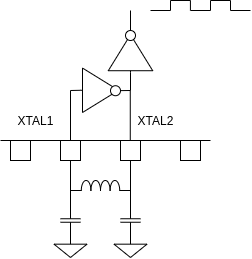
\includegraphics[width=200px]{images/17_Clock/basic_clock_generator.png}
\end{figure}
Tra i pin XTAL1 ed XTAL2 abbiamo un amplificatore invertente, XTAL1 è a alta impedenza mentre XTAL2 è a bassa impedenza.
Nella funzione di trasferimento del circuito abbiamo 3 poli in quanto abbiamo 3 elementi reattivi, quindi esiste una sola frequenza tale che la fase tra i due pin è 180°.
\begin{figure}[H]
    \centering
    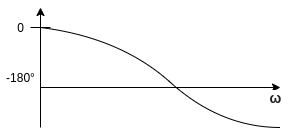
\includegraphics[width=300px]{images/17_Clock/frequency_response.png}
\end{figure}
Solo per la frequenza nella quale si ha l' intersezione il circuito è un oscillatore perfetto.
La frequenza alla quale si trova questa intersezione è fortemente dipendente dalla posizione dei poli, quindi dai valori degli elementi reattivi.

Per essere più precisi spesso si utilizza un cristallo risuonatore che ha una oscillazione ad una frequenza ben precisa: di solito si usa un cristallo di quarzo che essendo un elemento circuitale piezoelettrico ha una vibrazione meccanica facilmente prevedibile in base alla massa del cristallo.
\begin{figure}[H]
    \centering
    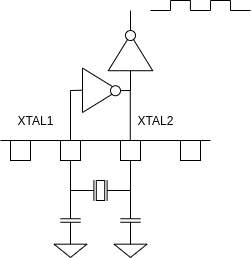
\includegraphics[width=200px]{images/17_Clock/crystal_oscillator.png}
\end{figure}
Il suo circuito equivalente è:
\begin{figure}[H]
    \centering
    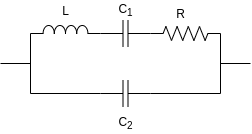
\includegraphics[width=200px]{images/17_Clock/equivalent_circuit.png}
\end{figure}
in cui:
\begin{itemize}
    \item $L$: è dovuto alla massa del cristallo, è come una molla
    \item $C_1$: è dovuto alla rigidità meccanica del pezzetto di cristallo
    \item $C_2$: dovuto alla capacità delle armature che ingabbiano il cristallo. $C_2 \sim 100C_1$
    \item $R$: corrisponde all' attrito che porterebbe a stoppare l' oscillazione
\end{itemize}
Approssimiamo l' impedenza del parallelo (trascuriamo la resistenza perché molto piccola):
\begin{itemize}
    \item in 0 abbiamo solo la capacità quindi abbiamo impedenza negativa
    \item la serie $L$ e $C_1$ si annulla quando sono uguali ed opposti, l' altro ramo è in parallelo quindi rimane zero, questa frequenza è $\omega_s$
    \item posso avere risonanza anche quando i due rami si annullano, questa frequenza la chiamiamo $\omega_p$
    \item sappiamo che $\omega_s < \omega_p$ e che in $\omega_p$ l' impedenza è infinita
\end{itemize}
\begin{figure}[H]
    \centering
    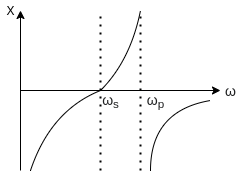
\includegraphics[width=200px]{images/17_Clock/impedence.png}
\end{figure}
Possiamo quindi dire:
\begin{itemize}
    \item $\omega < \omega_s$: è un condensatore
    \item $\omega > \omega_p$: è un condensatore
    \item $\omega_s < \omega < \omega_p$: è un induttore
\end{itemize}
Quindi all' interno di quel range il cristallo si comporta come un induttore, il range è tuttavia molto ristretto e molto preciso:
$$ |\omega_p - \omega_s| < 10^{-4} $$
Per esempio se: $\omega_s = 1$MHz allora $\omega_p = 1,0001$MHz quindi $\Delta{f} = 100$Hz è il range induttivo.
Abbiamo quindi un risuonatore con finestra di $100$Hz.

NB: i quarzi più economici di solito hanno $\Delta{f} = 30$Hz mentre quelli più costosi $\Delta{f} = 5$Hz.

Se volessi fare di meglio potrei utilizzare un cristallo termostatato cioè un cristallo a temperatura controllata e costante ottenuto usando una resistenza per mantenere la temperatura circa costante.


\subsubsection{Oscillatore a rilassamento}
Un altro oscillatore che possiamo utilizzare è quello a rilassamento:
\begin{figure}[H]
    \centering
    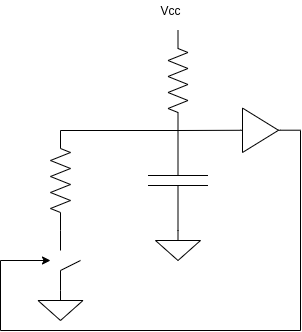
\includegraphics[width=150px]{images/17_Clock/relaxation_oscillator.png}
\end{figure}
Quando il condensatore si carica, lo facciamo caricare fino ai $\frac{2}{3}$, successivamente lo facciamo scaricare fino ai $\frac{1}{3}$ e così via ciclicamente.
\begin{figure}[H]
    \centering
    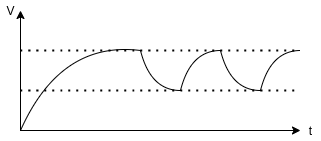
\includegraphics[width=200px]{images/17_Clock/relaxation_time_graph.png}
\end{figure}
La frequenza è esprimibile nella forma:
$$ f = \frac{\alpha}{RC} $$
ed è fortemente dipendente dalla precisione con la quale si scelgono i valori delle componenti, in genere va attorno al 1-3\%.

Nel nostro uC possiamo usare l'amplificatore che già c'è aggiungendo giusto un paio di componenti esterne:
\begin{figure}[H]
    \centering
    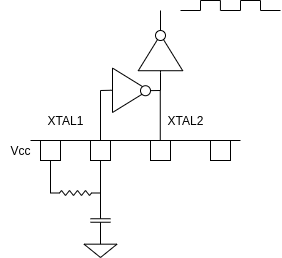
\includegraphics[width=200px]{images/17_Clock/relaxation_in_uC.png}
\end{figure}

Un' altra possibilità è quella di utilizzare la rete RC interna del uC.

\subsubsection{Clock esterno}
Possiamo usare un clock esterno direttamente inserito in XTAL1:
\begin{figure}[H]
    \centering
    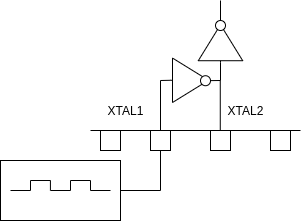
\includegraphics[width=200px]{images/17_Clock/external_clock.png}
\end{figure}
Questo è tipico dei sistemi a 2 uC in cui uno ha un generatore di clock con cristallo e l'altro usa il clock generato dal primo per funzionare:
\begin{figure}[H]
    \centering
    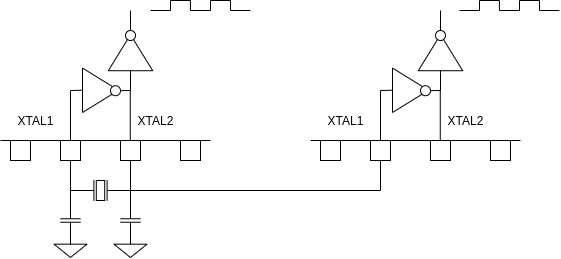
\includegraphics[width=300px]{images/17_Clock/back_to_back.png}
\end{figure}



\section{Timer}
L' ATMega32 è dotato di 3 timer interni:
\begin{itemize}
    \item timer 0
    \item timer 1
    \item timer 2
\end{itemize}
I timer 0 e 2 sono molto simili.

\subsection{Timer 0}
TCNT0 è un registro ad 8 bit, il suo valore è incrementato in maniera automatica tramite il clock o un suo derivato.
Posso scriverci un valore a piacere e leggere il valore corrente in qualsiasi momento.
Quando conta conta solo in avanti da 0 a 255, dopodiché si \emph{wrappa} e torna a 0 e così via.

\begin{figure}[H]
    \centering
    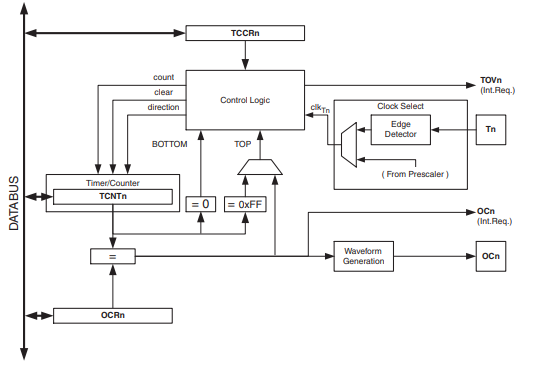
\includegraphics[width=300px]{images/18_Timer/Timer0.png}
\end{figure}

\subsubsection{Utilizzo come timer}
Incrementa il contatore ogni $\tau$ più o meno a scelta.
E' usato per misurare intervalli di tempo e se 256 valori non bastano si possono contare i wrap.
Più la frequenza è alta e più è alta la risoluzione ma più velocemente il contatore fa wrap!
Ogni volta che il contatore torna a 0 un' interruzione viene lanciata e può essere catchata per farci qualcosa.

In questa configurazione il clock è quello del processore, spesso tuttavia risulta troppo veloce, per rallentarlo possiamo usare il \emph{prescaler} integrato configurabile ai valori: 1, 8, 64, 256, 1024.

NB: il prescaler impostato ad 1 è il default ed implica che non ci sia un vero e proprio rallentamento del clock. 8, 64, ecc invece indicano che anziché aggiornare ad ogni tick del clock si aggiorna ogni 8, ogni 64, ecc, ecc.

\subsubsection{Utilizzo come contatore}
Conta gli eventi sporadici, l' aggiornamento non è periodico.
Per ottenere questa funzionalità il clock del contatore è esterno, un pin apposito del package

Per configurarlo in questo modo bisogna collegare l' ingresso esterno T0 all' ingresso del contatore.

\subsubsection{Comparatore}
All' interno della struttura del timer esiste un altro registro: OCR0, una volta asegnatogli un valore esso vi rimane, ogni volta che TCNT0 viene incrementato una rete combinatoria controlla se il valore corrente è uguale al contenuto di OCR0, se combaciano viene lanciata una interruzione.
Un utilizzo tipico è quello di contare intervalli costanti:
\begin{itemize}
    \item setto OCR0 a 70
    \item abilito il clock su TCNT0
    \item quando TCNT0 sta transitando da 70 a 0 arriva l'interrupt (ho ottenuto un \emph{match})
    \item nel gestore dell' interruzione azzero TCNT0 per fargli contare di nuovo un intervallo fisso
\end{itemize}
La stessa rete combinatoria che mi lancia l' interruzione può ripulire il registro TCNT0, quindi questo conteggio può essere eseguito in automatico.

Questo segnale di match può essere anche usato per alterare lo stato del pin di uscita OC0:
\begin{itemize}
    \item alzare OC0
    \item abbassare OC0
    \item toggle di OC0 (cioè commutare lo stato corrente)
\end{itemize}

Possiamo ad esempio generare un' onda quadra ad una certa frequenza: supponiamo di voler generare un' onda quadra a 400Hz, il periodo deve essere di $T = \frac{1}{400 Hz} = 2.5 ms = 2500 \mu s$.
Supponiamo di avere $f_{ck} = 1 MHz$ e quindi periodi di $1\mu s$, ci serve avere un match ogni $\frac{T}{2} = 1250\mu s$ cioè un match ogni 1250 cicli di clock.
% TODO disegno onda quadra con periodi %
Usando un prescaler ad 8 mi serve un match ogni $\frac{1250}{8} = 156,25$, arrotondiamo a 156, quindi in OCR0 andrò ad inserire il valore 156.
Per la precisione il match è ogni $1248\mu s$ quindi perdo $4\mu s$ ad ogni periodo.
Se usassi il prescaler a 64 in OCR0 dovrei metterci 20 ma facendo i conti il valore corretto sarebbe 19.53 quindi ho un errore sul periodo più grande. 

Il prescaler a valori alti serve per $f_{ck}$ alto o per periodi lunghi.

Es: $f = 30KHz$, $T = 33\mu s$, $\frac{T}{2} = 16.6\mu s$ \\
$f_{ck} = 1MHz$, $T = 1\mu s$, OCR0 va settato a 17 \\

Imposto poi che ad ogni match ci sia il toggle di OC0 e quindi ho la nostra onda quadra in uscita.
Se volessi farlo fermare dopo 100 volte potrei abilitare l' interruzione sul wrap e dopo 100 volte che l' interruzione scatta disabilitare il clock al timer.

NB: se voglio contare 70 in OCR0 ci devo mettere 69, questo perché la comparazione è eseguita al nuovo cambio di valore!

\subsubsection{Configurazione}
I bit utili per la configurazione del timer 0 si trovano all' interno di TCCR0, in particolare:
\begin{figure}[H]
    \centering
    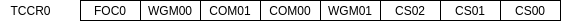
\includegraphics[width=320px]{images/18_Timer/TCCR0.png}
\end{figure}
\begin{itemize}
    \item CS02, CS01, CS00: selezionano il clock da usare per contare
    \item WGM01, WGM00: selezionano la modalità di funzionamento tra timer e counter
    \item COM01, COM00: selezionano il tipo di aggiornamento del pin OC0 in caso di match
    \item FOC0: si usa per generare un match finto, aggiorna l' uscita OC0 in base alla configurazione ma non azzera il contatore, né fa scattare l' interrupt
\end{itemize}

Per abilitare le interruzioni della periferica si usa il registro TIMSK:
\begin{figure}[H]
    \centering
    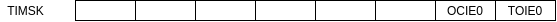
\includegraphics[width=320px]{images/18_Timer/TIMSK.png}
\end{figure}
\begin{itemize}
    \item TOIE0: abilita l' interruzione al wrap
    \item OCIE0: abilita l' interruzione sul match
\end{itemize}
I bit di flag invece si trovano in TIFR:
\begin{figure}[H]
    \centering
    \includegraphics[width=320px]{images/18_Timer/TIFR.png}
\end{figure}
\begin{itemize}
    \item OCF0: flag dell' interrupt sul match
    \item TOV0: flag dell' interrupt sul wrap
\end{itemize}

\subsubsection{Esempio: orologio di sistema}
Inseriamo il prescaler massimo , quindi ad ogni wrap interrupt saranno passati $256 \cdot 1024 = 2^{18}$ cicli di clock, supponendo che $T_{ck} = 1\mu s$ ad ogni interrupt saranno passato $2^{18}\mu s$.
Ogni milione di cicli di clock invece è passato 1 secondo, quindi quando scatta l' interruzione aggiorno un contatore, e se è passato oltre 1M scalo 1M ed aggiorno il valore della variabile secondi, e così via per il resto. 


\subsection{Timer 1}
E' un timer a 16 bit quindi possiamo aspettare tempi più lunghi con un prescaler minore, abbiamo una risoluzione maggiore.
Essendo a 16 bit ogni registro di utilità è in realtà composto da due registri:
\begin{figure}[H]
    \centering
    \includegraphics[width=200px]{images/18_Timer/TCNT1.png}
\end{figure}

\subsubsection{Comparatore}
Abbiamo due registri di comparazione:
\begin{figure}[H]
    \centering
    \includegraphics[width=200px]{images/18_Timer/OCR1A.png}
\end{figure}
\begin{figure}[H]
    \centering
    \includegraphics[width=200px]{images/18_Timer/OCR1B.png}
\end{figure}
tuttavia il reset al match può essere configurato solo per OCR1A quindi se si devono usare entrambi i comparatori conviene inserire valori tali che OCR1B $<$ OCR1A in quanto altrimenti il primo match resetta il contatore ed il secondo match non si avrà mai!

Abbiamo due pin di uscita da poter modificare al match: OC1A ed OC1B associati ad OCR1A ed OCR1B.
Abbiamo ovviamente due bit di controllo per ogni OCR1.

\subsubsection{Trigger esterno}
Nel package esiste un pin ICP1 (Input Capture Pin) ed il registro ICR1H/L:
\begin{figure}[H]
    \centering
    \includegraphics[width=200px]{images/18_Timer/ICR1.png}
\end{figure}
quando arriva un impulso sul pin ICP si copia il valore di TCNT1 in ICR1.
Possiamo implementare una specie di photofinish.

Si noti che è previsto anche che ICR1 possa essere usato come registro di match.

Es: con 16MHz di clock abbiamo una risoluzione di $T_R = 62,5 ns$, la velocità del suono è $V_{suono} = 340 \frac{m}{s}$ quindi la distanza percorsa in ogni istante misurato dal timer è di:
$d = 340 \times 62,5 \times 10^{-9} = 21,25 \mu m$
Possiamo misurare la distanza con una risoluzione di $21,25\mu m$ usando un radar sonoro.

\subsubsection{Cancellazione del rumore}
Attaccato al pin ICP1 c'è un circuito per la cancellazione del rumore:
\begin{figure}[H]
    \centering
    \includegraphics[width=250px]{images/18_Timer/noise_reduction_circuit.png}
\end{figure}
tengo in memoria il valore del pin ICP negli ultimi 4 clock, se è sempre stato ad 1 la porta AND lo rileva e scatta il trigger.

Questo circuito può essere utile ad esempio quando abbiamo inserito un interruttore meccanico per triggerare il pin ICP1, può succedere che in fase di chiusura non ci sia una transisione netta dal livello logico 0 al livello logico 1, piuttosto degli spike, sono dette \emph{alee}. Con questo circuito limitiamo enormemente il loro impatto.
E' anche detto \emph{debouncing} hardware, questo aggiunge un ritardo di 4 clock.
il valore della AND è poi inserito in un multiplexer per poter scegliere se triggerare la cattura del contatore sul livello logico basso o sul livello logico alto.

\subsubsection{Letture e scritture atomiche}
Essendo il contatore locato su due indirizzi per leggere dobbiamo eseguire due letture distinte, se lo facciamo mentre il timer corre potremmo avere dei problemi:
\begin{itemize}
    \item valore timer: 0x00FF, leggo la parte bassa ed ottengo 0xFF
    \item il clock incrementa il timer
    \item valore timer: 0x0100, leggo la parte superiore ed ottengo 0x01
    \item ho quindi letto 0x01FF, ho un errore enorme sul reale valore del timer
\end{itemize}
oppure:
\begin{itemize}
    \item valore timer: 0x00FF, leggo la parte alta ed ottengo 0x00
    \item il clock incrementa il timer
    \item valore timer: 0x0100, leggo la parte inferiore ed ottengo 0x00
    \item ho quindi letto 0x0000, anche qui un grande errore
\end{itemize}

Servirebbe poter leggere due indirizzi nello stesso ciclo di clock ma non possiamo farlo.
Per fortuna l'hardware del timer ci viene in aiuto:
\begin{figure}[H]
    \centering
    \includegraphics[width=250px]{images/18_Timer/atomic_read.png}
\end{figure}
\begin{itemize}
    \item nella prima lettura leggo direttamente la parte bassa che mi viene copiata nel registro r16, sempre durante questa lettura la parte alta viene letta ed inserita automaticamente in un registro temporaneo
    \item eseguendo la lettura della parte alta in realtà mi viene consegnato il valore inserito nel registro temporaneo
\end{itemize}
in questo modo ho ottenuto una lettura atomica.

Questa procedura è eseguita automaticamente per ogni registro a 16 bit della periferica quindi: \emph{per leggere un registro a 16 bit si deve prima leggere la parte bassa e poi la parte alta}, fare il contrario fornisce sicuramente risultati sbagliati.
Inoltre non si deve mai interrompere una lettura, se leggo il byte basso di qualche registro devo poi leggere anche la parte alta.

Si noti che continuano ad esserci problemi se entrano in gioco anche le interruzioni: ad esempio se leggo la parte bassa, e quindi l' alta mi viene messa nel registro temporaneo, ma poi parte una interruzione che legge i registri del timer, allora il registro temporaneo sarà stato sporcato e quindi la successiva lettura sarà sbagliata.

\emph{Le scritture vanno eseguite in maniera big endian cioè prima va scritta la parte alta, che verrà inserita nel registro temporaneo, e successivamente nella parte bassa}, solo a questo punto avviene la vera scrittura nel registro del timer.


\subsubsection{Configurazione}
I registri di controllo sono tutti su 8 bit e sono TCCR1A, TCCR1B, TCCR1C:
\begin{figure}[H]
    \centering
    \includegraphics[width=320px]{images/18_Timer/TCCR1A.png}
\end{figure}
\begin{itemize}
    \item COM1Ax: indicano cosa fare al match con OCRA
    \item COM1Bx: indicano cosa fare al match con OCRB
    \item FOC1x: quando vengono settati lanciano un match parziale, quindi agiscono sul pin OC1A ed OC1B, ma senza lanciare l' interruzione
    \item WGM1x: indicano la modalità di funzionamento del timer
\end{itemize}

\begin{figure}[H]
    \centering
    \includegraphics[width=320px]{images/18_Timer/TCCR1B.png}
\end{figure}
\begin{itemize}
    \item WGM1x: assieme ai bit WGM1x in TCCR1A configurano la modalità di funzionamento del timer
    \item ICNC1: abilita/disabilita la noise reduction
    \item ICES1: indica su quale fronte di ICP1 triggerarsi
    \item CS1x: selezionano il clock + prescaler da usare per aggiornare il contatore
\end{itemize}

\begin{figure}[H]
    \centering
    \includegraphics[width=320px]{images/18_Timer/TIMSK_1.png}
\end{figure}
\begin{itemize}
    \item TICIE1: abilita l' interruzione sul cambiamento di valore sul pin ICP1
    \item OCIE1A: abilita l' interruzione sul match con OCRA
    \item OCIE1B: abilita l' interruzione sul match con OCRB
    \item TOIE1: abilita l' interruzione al wrap del timer
\end{itemize}

I bit di flag invece si trovano in TIFR:
\begin{figure}[H]
    \centering
    \includegraphics[width=320px]{images/18_Timer/TIFR_1.png}
\end{figure}
\begin{itemize}
    \item ICF1: flag dell' interrupt sulla modifica del pin ICP1
    \item OCF1A: flag dell' interrupt sul match con OCR1A
    \item OCF1B: flag dell' interrupt sul match con OCR1A 
    \item TOV1: flag dell' interrupt sul wrap
\end{itemize}

\subsection{Timer 2}
Funziona come il timer 0, abbiamo quindi i registri:
\begin{itemize}
    \item TCNT2: registro contatore
    \item OCR2: registro di match 
    \item TCCR2: registro di controllo
\end{itemize}

Il timer 2 può essere usato in maniera asincrona cioè può essere aggiornato da un clock differente da quello della CPU.
In particolare è pensato per un oscillatore al quarzo per orologi (cioè a $2^{15}Hz$) inserito tra i pin TOSC1 e TOSC2 con lo stesso circuito visto per il clock generale.

Questa funzionalità è usata principalmente per poter staccare il clock originale e risparmiare energia dormendo per tempi più lunghi grazie alla bassa frequenza dell' oscillatore.

Es: ci risvegliamo dopo 255 conteggi ad una frequenza di $2^{15}Hz$ ed un prescaler di 1024. Si ha quindi una frequenza per l' aggiornamento del contatore di $\frac{2^{15}}{2^{10}} = 2^{5} = 32Hz$, per un wrap ci vogliono $\frac{256}{32Hz} = 8s$.

Dato che il clock di questo timer è asincrono potrebbe succedere di scrivere in uno dei suoi registri varie volte nello stesso ciclo di clock asincrono.
Questo è un problema in quanto renderebbe inconsistente qualsiasi scrittura che si sta eseguendo.

Per queste proprietà peculiari del timer esiste un registro di controllo a se:
\begin{figure}[H]
    \centering
    \includegraphics[width=320px]{images/18_Timer/ASSR.png}
\end{figure}
\begin{itemize}
    \item AS2: abilita la modalità asincrona
    \item TCN2UB: quando è ad 1 indica che c'è già stata una scrittura su TCNT2 e quindi non si dovrebbe farne un' altra
    \item OCR2UB: quando è ad 1 indica che c'è già stata una scrittura su OCR2 e quindi non si dovrebbe farne un' altra
    \item TCR2UB: quando è ad 1 indica che c'è già stata una scrittura su TCCR2 e quindi non si dovrebbe farne un' altra
\end{itemize}
NB: UB sta per update busy, i bit busy vanno a 0 quando la scrittura è effettivamente avvenuta.



\section{PWM - Pulse Width Modulation}
\subsection{Introduzione}
E' un tipo di modulazione utilizzato largamente nell' elettronica di potenza.
In genere se si vuole comandare la tensione ai capi di un carico si deve ricorrere ad un circuito del genere:
\begin{figure}[H]
    \centering
    \includegraphics[width=150px]{images/19_PWM/power_dimmer.png}
\end{figure}
Quando si applica una tensione $V$ nell' ingresso non invertente dell' opamp per il cortocircuito virtuale ce l' abbiamo anche nell' ingresso invertente, quindi anche al capo della resistenza R.
Supponiamo di avere $V_{dd} = 12V$, $R = 1 \Omega$ e di applicare $V = 12V$ allora la potenza dissipata sulla resistenza $R$ è: $P = RI^2 = R \cdot \left( \frac{V}{R} \right)^2 = 144W$, se la tensione ai capi della resistenza è troppo grande possiamo abbassarla, supponiamo di variarla a $V = 6V$ la corrente che scorre in $R$ adesso è $I = \frac{V}{R} = 6A$ tuttavia ora molta potenza è dissipata anche sul transistor infatti abbiamo che $V_{CC} \cdot I_C = 36W$.

Se voglio evitare di dissipare potenza sul controllore (il transistor) devo passare ad un circuito con un transistore usato come interruttore:
\begin{figure}[H]
    \centering
    \includegraphics[width=20px]{images/19_PWM/dimmer_with_switch.png}
\end{figure}
in questo modo quando chiudo il circuito ho una corrente di 12A, quando apro il circuito ho 0A, se volessi avere 6A potrei aprire per metà del tempo e chiudere per l' altra metà del tempo:
\begin{figure}[H]
    \centering
    \includegraphics[width=320px]{images/19_PWM/duty_cycle.png}
\end{figure}
chiamiamo $t_{ON}$ il tempo in cui il circuito è chiuso e $t_{OFF}$ il tempo in cui il circuito è aperto allora definiamo:
$$ \delta = \frac{t_{ON}}{t_{ON} + t_{OFF}} = \text{duty cycle} $$

Uno degli inconvenienti di questo approcio è che il dispositivo alimentato non è effettivamente alimentato con una tensione intermedia ma acceso per un po' di tempo e spento per un altro po' di tempo, per alcuni carichi questo non è un problema (luci, led, motori, resistori per forni) per altri risulta essere problematico.

Calcoliamo la potenza lungo tutto il periodo: supponiamo che quando il transistor è chiuso si abbia potenza $P_0$ : 
$$ P = \frac{P_0 \cdot T_{ON} + 0 \cdot T_{OFF}}{T_{ON} + T_{OFF}} = P_0 \cdot \delta $$
la potenza sul carico è direttamente proporzionale a $\delta$ con $0 \leq \delta \leq 1$.
Si noti che questa è una potenza media in quanto calcolata su un intervallo.

La modulazione fatta in questo modo è semplice se eseguita da un microcontrollore, ovviamente si può fare senza logica con comparatori e maglie RC ma il circuito risulta più complesso.

Lo stesso segnale PWM generato posso usarlo per pilotare il controllore tradizionale, per fare ciò bisogna trasformare il segnale PWM in un segnale continuo, lo spettro dell' onda quadra generata è così composto:
\begin{figure}[H]
    \centering
    \includegraphics[width=200px]{images/19_PWM/pwm_spectre.png}
\end{figure}
abbiamo quindi le armoniche dispari ma anche una componente, il valore medio dell'onda, che è anche l'unica componente che ci interessa.

Per eliminare l' armonica fondamentale e tutte le altre successive usiamo un filtro passa basso che abbia frequenza di taglio minore della frequenza fondamentale: $F_H < F$, tipicamente $F_H = \frac{F}{10}$.
\begin{figure}[H]
    \centering
    \includegraphics[width=200px]{images/19_PWM/ideal_filter.png}
\end{figure}
Ovviamente filtri del genere non esistono quindi ci affidiamo ad un filtro con un singolo polo che abbia una risposta in frequenza simile:
\begin{figure}[H]
    \centering
    \includegraphics[width=200px]{images/19_PWM/actual_filter.png}
\end{figure}
Possiamo usare questo stesso valore continuo per pilotare il controllore analogico visto in precedenza.

Es: creiamo un dimmer led, comandiamo la corrente nel diodo luminoso, dato che la sua luce è proporzionale alla corrente possiamo scegliere l' intensità luminosa del LED.
$$ I = \frac{\delta \cdot V_{dd}}{R} $$
\begin{figure}[H]
    \centering
    \includegraphics[width=200px]{images/19_PWM/pwm_led_dimmer.png}
\end{figure}

\subsection{Fast PWM}
Nel nostro microcontrollore il generatore PWM è costituito dal timer.
Preso un timer esso conta liberamente in avanti prima di tornare a 0:
\begin{figure}[H]
    \centering
    \includegraphics[width=200px]{images/19_PWM/fast_pwm_tcnt.png}
\end{figure}
in OCR ci mettiamo un valore ad 8 bit, quando il timer ha un valore minore di OCR in uscita poniamo 0, quando il valore in TCNT0 è maggiore di OCR mettiamo in uscita 1, oppure il contrario.
\begin{figure}[H]
    \centering
    \includegraphics{images/19_PWM/non_inverting-inverting_fast_pwm.png}
\end{figure}
In alto modalità NON invertente, in basso modalità invertente.

All' aumentare di OCR0:
\begin{itemize}
    \item nella modalità NON invertente il $T_{ON}$ aumenta, quindi $\delta$ aumenta
    \item nella modalità invertente il $T_{ON}$ diminuisce, quindi $\delta$ diminuisce
\end{itemize}

Dato che i valori sono interi non possiamo avere tutti i valori possibili di $\delta$, la risoluzione del periodo è $\Delta\delta = \frac{1}{256} = 0.4\%$.

Il periodo di questo PWM è $T = 256 \cdot t_{CK} \cdot P$ in cui $t_{CK}$ è il periodo del clock mentre $P$ è il valore corrente del prescaler, quindi 1, 8, 64, 256 o 1024.

La frequenza massima si ha per $t_{CK}$ minima e $P=1$, usando il timer0 con clock di 1MHz $t_{CK} = 1 \mu s$ quindi il periodo è di $256 \mu s$ quindi la frequenza è $f = \frac{1}{256\mu s} = 4KHz$.
Volendo uscire dalla banda audio si deve andare oltre i 20KHz, usando clock a 4MHz la frequenza è già $f = 16KHz$ che è ai limiti della banda audio, solitamente udibile da ben poche persone, quindi va già bene.

Usando il timer1 non si ha un conteggio a 16 bit, se lo facesse si avrebbe una frequenza PWM bassissima, ad esempio con clock a 1MHz la frequenza sarebbe $f = \frac{1}{256^2 \mu s} = 15Hz$, per evitare ciò si è pensato di dotare il timer1 di 3 modalità PWM che permettono di avere risoluzioni a:
\begin{itemize}
    \item 8 bit: 0-255
    \item 9 bit: 0-511
    \item 10 bit: 0-1023
\end{itemize}
Es: a 10 bit $\Delta \delta = 0.001$ ma la frequenza diminuisce in quanto il periodo aumenta di 4 volte.

Nella maggior parte dei casi l' importante è avere una frequenza alta e non una risoluzione alta.

Abbiamo in totale 4 generatori PWM indipendenti:
\begin{itemize}
    \item timer 0 ha 1 generatore PWM ad 8 bit
    \item timer 1 ha 2 PWM con OCRA ed OCRB
    \item timer 2 ha 1 generatore PWM identico a quello di timer 0
\end{itemize}

\begin{figure}[H]
    \centering
    \includegraphics[width=200px]{images/19_PWM/pwm_timer_1.png}
\end{figure}

\subsection{PWM a fase corretta}
Essendo un segnale rettangolare il baricentro degli impulsi si trova nel centro del rettangolo.
Facendo la trasformata di Fourier del segnale la componente sinusoidale fondamentale ha questa forma:
\begin{figure}[H]
    \centering
    \includegraphics[width=200px]{images/19_PWM/pwm_center_of_gravity.png}
\end{figure}
Il massimo della sinusoide è nel baricentro del $T_{ON}$, il minimo è nel baricentro del $T_{OFF}$, che sono spaziati di un semiperiodo.
Se vario OCRA il margine destro dell' impulso si sposta e con lui anche il baricentro, quindi la sinusoide: cambiano le fasi delle armoniche che costituiscono il segnale.

In certe applicazioni la fase del segnale è importante, ad esempio se abbiamo due motori che sono alimentati da due segnali diversi alla stessa frequenza in base alla fase di ogni segnale abbiamo che i disturbi dei due motori possono sommarsi oppure cancellarsi l' uno con l' altro.

Se non si vogliono avere problemi di sorta con la fase del segnale anziché usare il fast PWM possiamo passare al PWM a fase corretta.

In questa modalità il contatore conta up-down, cioè prima conta da 0 a 255 e poi da 255 a 0:
\begin{figure}[H]
    \centering
    \includegraphics[width=200px]{images/19_PWM/phase_correct_pwm.png}
\end{figure}
in questa modalità se cambio OCR a spostarsi sono entrambi i lati del rettangolo $T_{ON}$ quindi il baricentro rimane fermo.
Tuttavia il periodo questa volta è raddoppiato in quanto dobbiamo contare il doppio:
$$ T = 2 \cdot 256 \cdot t_{CK} \cdot P $$

\subsection{Glitch}
Se cambio la configurazione del timer mentre è in corso potrebbe accadere che in alcuni periodi si abbiano due $T_{ON}$, per evitare ciò si consiglia di aggiornare i registri quando il contatore è al massimo o al minimo.

\subsection{Configurazione nel uC}
\subsubsection{Timer 0}
Per configurare quale modalità PWM si usano i bit WGM:
\begin{table}[H]
    \centering
    \begin{tabular}{c c | l}
        WGM01 & WGM00 & Descrizione \\
        \hline
        0 & 1 & PWM a fase corretta \\
        \hline
        1 & 1 & Fast PWM \\
        \hline
    \end{tabular}
\end{table}
Per configurare l' inversione del PWM si usano i bit COM00 e COM01:
\begin{table}[H]
    \centering
    \begin{tabular}{c c | l}
        COM01 & COM00 & Descrizione \\
        \hline
        0 & 0 & OC0 disconnesso \\
        \hline
        0 & 1 & - \\
        \hline
        1 & 0 & NON invertente \\
        \hline
        1 & 1 & invertente \\
        \hline
    \end{tabular}
\end{table}
il clock si sceglie sempre tramite i bit CS.

\subsubsection{Timer 1}
Per il timer 1 valgono le stesse considerazioni ma abbiamo molte più configurazioni del PWM perché possiamo usarlo a 8, 9, 10 bit.

\subsubsection{Timer 2}
Il timer 2 è identico al timer 1 con l' aggiunta della possibilità di usare una sorgente esterna come clock del timer.


\section{GPIO}
La periferica GPIO - General Purpose Input/Output ci permette di programmare alcuni pin del uC e di imporre un valore logico, oppure di leggere il valore logico che c'è su un pin.
Ci permettono in pratica di interfacciarci con il mondo esterno.

\subsection{Output}
\subsubsection{Direzione della corrente}
Configurati come output posso imporre il valore logico 1 oppure 0:
\begin{figure}[H]
    \centering
    \includegraphics[width=150px]{images/21_GPIO/gpio_output_current.png}
\end{figure}
Se impongo 1 logico il pin può fornire corrente, infatti nel caso a sinistra quando poniamo 1 il led si accende.
Se impongo 0 logico il pin può assorbire corrente, infatti nel caso a destra quando poniamo 0 il led si accende. 

NB: Far passare la corrente nel senso contrario a quello previsto dal pin potrebbe danneggiare il componente, ad esempio se poniamo in uscita 1 logico ma all' altro capo del resistore poniamo 7V abbiamo che la corrente è in ingresso al pin, mentre dovrebbe essere in uscita.

\subsubsection{Struttura interna}
\begin{figure}[H]
    \centering
    \includegraphics[width=150px]{images/21_GPIO/gpio_output_circuit.png}
\end{figure}
Il MOS in alto è un P-channel quello in basso è un N-channel.
Se chiudo il primo ed apro il secondo pongo 1 in uscita, se apro il primo e chiudo il secondo pongo 0 in uscita. 

NB: I due MOS non possono mai essere chiusi insieme, se succedesse avrei un cortocircuito nel chip e sarebbe dannoso.

I due diodi sono diodi di protezione, intervengono in caso la corrente all' interno del pin giri nel senso opposto a quello previsto canonicamente:
\begin{figure}[H]
    \centering
    \includegraphics[width=150px]{images/21_GPIO/protection_diode.png}
\end{figure}
Hanno una certa tolleranza che ci può aiutare in caso di errore, tuttavia sono pensati per far si che le scariche elettrostatiche sui pin non danneggino l' interno del chip, sono infatti diodi anti-ESD (electrostatic discharge).

Il resistore in serie al pin è usata per evitare che carichi a bassa impedenza chiedano troppa corrente e danneggino i MOS, è current limiting resistor.

Il condensatore in parallelo all' uscita invece è un condensatore parassita, non è pertanto desiderato ma è presente per costruzione.

\subsubsection{Pilotare carichi}
Per pilotare carichi usando i GPIO conviene usare i livelli logici come ingresso per qualche amplificatore, banalmente dei transistori:
\begin{figure}[H]
    \centering
    \includegraphics[width=250px]{images/21_GPIO/pilotare_carichi.png}
\end{figure}
Questo perché ogni pin può emettere al massimo 20mA ed in totale, tra tutti i pin come uscita, non si può emettere più di 200mA perché è la limitazione del pin di alimentazione del uC.

All' occorrenza potrebbe essere necessario però avere in uscita più di 20mA, ad esempio se vogliamo alimentare un LED in modo che si veda la sua luce anche di giorno bisogna dargli almento 30mA.
Possiamo pensare di usare 2 pin come uscita e sincronizzare il loro livello logico, in questo modo quando diamo livello alto su entrambe le uscite possiamo arrivare ad un massimo di 40mA:
\begin{figure}[H]
    \centering
    \includegraphics[width=100px]{images/21_GPIO/pin_in_parallelo_led.png}
\end{figure}
vediamo internamente cosa comporta questa connessione:
\begin{figure}[H]
    \centering
    \includegraphics[width=150px]{images/21_GPIO/pin_in_parallelo_internal.png}
\end{figure}
Per far scorrere 30mA supponendo una caduta di tensione ai capi del led di $V_{\gamma} = 2.1V$:
$$ V_{R} = 5 - V_{\gamma} = 5-2.1 = 2.9V $$
$$ R = \frac{V}{I} = \frac{2.9V}{30mA} \approx 100 \Omega $$
quindi dobbiamo usare due resistori da 200$\Omega$ in modo che in parallelo diano 100$\Omega$.
Tutto questo ragionamento vale assumendo che la corrente arrivi in uguale misura da entrambi i pin, usando i MOS questa assunzione risulta vera perché se uno dei due rami fa scorrere più corrente porterà il MOS di quel ramo a riscaldarsi di più e quindi a condurre meno e dunque a trasportare meno corrente, si finisce quindi ad avere circa un pareggio.
Usando dei BJT invece questa assunzione non è vera perché i transistori bipolari con l' aumento della temperatura conducono di più, il che potrebbe portare al \emph{current hobbing}.

Devo fare attenzione ad ogni modo a non assegnare livello logico alto ad un pin e basso ad un altro pin perché crerei un corto circuito nell' alimentazione del uC, il che porterebbe a danneggiare i MOS o a scaricare l' eventuale batteria che alimenta il uC.
Le resistenze che abbiamo inserito possono aiutare anche in questa situazione poiché figurano come in serie ed abbiamo una limitazione alla corrente nel cortocircuito.
Un' altra soluzione è quella di inserire all' uscita dei pin dei diodi e la loro uscita inserirla in parallelo, in questo caso bisogna ricordare la caduta di tensione dei diodi.

Anche in caso usassi uscite di due uC diversi dovrei proteggerne almeno una con un resistore:
\begin{figure}[H]
    \centering
    \includegraphics[width=100px]{images/21_GPIO/uscite_uC_diversi_in_parallelo.png}
\end{figure}
in questo caso si viene a creare una maglia RC con le capacità parassite, questo porta alla creazione di un limite superiore per la banda del sistema, quindi potrebbe rallentarlo.

\subsection{Input}
I pin possono anche essere configurati come ingresso.
Supponiamo di voler testare lo stato di un pulsante, possiamo usare i seguenti circuiti:
\begin{figure}[H]
    \centering
    \includegraphics[width=200px]{images/21_GPIO/pull-up_pull-down.drawio.png}
\end{figure}
\begin{itemize}
    \item sulla sinistra abbiamo la confgiurazione con resistore in pull-up, quando il circuito è aperto e dunque il pulsante non è premuto abbiamo valore logico alto.
    Quando il pulsante è premuto sul pin abbiamo valore logico basso.
    
    \item sulla destra abbiamo la configurazione con resistore in pull-down, quando il circuito è aperto e dunque il pulsante non è premuto abbiamo valore logico basso.
    Quando il pulsante è premuto sul pin abbiamo valore logico alto.
\end{itemize}
In entrambi i casi il resistore si inserisce di valore alto in modo che la corrente che scorre in ingresso al pin sia piccola, però non deve neanche essere troppo alto perché la capacità parassita interna ha necessità di caricarsi e se la resistenza è troppo grande il tempo di caricamento anche è grande.
Per esempio: avendo $C = 10^{-11}F$ e $R=10^4 \Omega$ abbiamo che: $\tau = 10^{-11} \cdot 10^{4} = 10^{-7}s = 100 ns$
in questo caso il tempo di caricamento è trascurabile rispetto al clock.

Se non inserissi il resistore per fare pull-up/pull-down quando il circuito è chiuso ho un valore logico stabile, quando ce l' ho aperto il valore logico dipende da quanto è carica la capacità interna!

Il resistore di solito si inserisce di valore nel range di 10K - 47K.

\subsubsection{Struttura interna}
\begin{figure}[H]
    \centering
    \includegraphics[width=150px]{images/21_GPIO/gpio_input_internals.drawio.png}
\end{figure}
Il buffer amplificatore legge il valore dall' esterno e permette al microcontrollore di leggerlo senza repentine modifiche della tensione.

Data questa struttura interna i pin sono più sicuri se impostati come input, possono essere messi in parallelo senza alcun problema.
Quando non vanno usati conviene sempre configurarli come ingresso, infatti al reset sono tutti impostati come pin di ingresso.

Si noti che i due circuiti di output ed input sono attivi allo stesso tempo, quindi i pin configurati come uscita possono comunque essere letti come ingresso:
\begin{figure}[H]
    \centering
    \includegraphics[width=175px]{images/21_GPIO/gpio_input_output.drawio.png}
\end{figure}

\subsubsection{Detect di un corto circuito tra i pin}
Dato che i pin possono essere configurati come uscita pur rimanendo come pin di ingresso possiamo usare questa feature per fare detecting di condizioni critiche:
\begin{figure}[H]
    \centering
    \includegraphics[width=200px]{images/21_GPIO/short_circuit_detection.png}
\end{figure}
essendo il MOS superiore chiuso ed il MOS inferiore spento abbiamo che l' uscita è impostata ad 1, tuttavia il pin è messo a ground.
Eseguendo una lettura del valore sul pin otteniamo infatti 0, siccome lo stato impostato in uscita è diverso da quello letto possiamo dire che c'è un cortocircuito sul pin.

Un problema del genere si ha anche quando ho due pin in parallelo ed ognuno ha in uscita un valore diverso, in tal caso il valore che vince il N-MOS e da lui il valore al canale.
Misuro le uscite e se sono diverse dal valore impostato come output allora abbiamo un cortocircuito.

\subsection{Registri}
I GPIO sono in totale 32 e sono divisi in gruppi da 8 in 4 batterie di registri diversi, ogni gruppo di 8 pin è detto \emph{porta}.
Abbiamo quindi:
\begin{itemize}
    \item Porta A: PA0, PA1, \_, PA7
    \item Porta B: PB0, PB1, \_, PB7
    \item Porta C: PC0, PC1, \_, PC7
    \item Porta D: PD0, PD1, \_, PD7
\end{itemize}

Ogni porta ha 3 registri di controllo e la posizione di ogni bit è riferita al pin che riguarda, es: il bit 0 dei registri di A riguardano tutti PA0,  

\subsubsection{DDRx}
E' il data direction register, se il bit è impostato ad 1 il pin è di uscita, se è a 0 il pin è di ingresso.

\subsubsection{PINx}
Se DDRx è impostato come input PINx indica il valore in ingresso su quel pin:
\begin{verbatim}
    IN r16, PINA
    ANDI r16, (1 << PA1)
\end{verbatim}

\subsubsection{PORTx}
Se DDRx è impostato come output in PORTx si inseriscono gli stati dei pin di uscita.
\begin{verbatim}
    LDI r16, (1 << PA0)
    OUT PORTA, r16
\end{verbatim}

\subsubsection{Pullup integrato}
C'è un resistore di pullup integrato per ogni pin, abbiamo la possibilità di abilitarlo e disabilitarlo a piacere.
Se il pin è impostato come input i bit di PORTx sono usati per indicare lo stato del pullup: 1 se deve essere abilitata, 0 se deve essere disabilitata.
Il resistore ha valore tra i 50k ed i 500k.

Inoltre il bit PUD (pull-up disable) può essere utilizzato per disabilitare globalmente i resistori di pull-up.

\subsubsection{Struttura interna}
\begin{figure}[H]
    \centering
    \includegraphics[width=330px]{images/21_GPIO/gpio_internal_structure.png}
\end{figure}
Quindi il resistore di pull-up è attivo se e solo se:
PUD = 0, DDRx = 0, PORTx = 1.

Per la lettura del valore in ingresso si usa un synchronizer per tenere stabile il valore di ingresso al flip flop di sampling perché il campionamento avviene all' atto della lettura del pin, non viene memorizzato periodicamente.

Si noti inoltre che prima del synchronizer vi è posto uno schmitt trigger.
Il valore in ingresso sul pin potrebbe non essere stabile al valore da campionare, anzi in genere oscilla abbastanza.
E' quindi necessario specificare per quale valore di tensione leggiamo 0 e per quale leggiamo 1, possiamo pensare di dividere il range della tensione con una soglia secca ma potrebbe essere problematico:
\begin{figure}[H]
    \centering
    \includegraphics[width=250px]{images/21_GPIO/single_threshold.png}
\end{figure}
abbiamo una traduzione che risente molto delle oscillazioni del segnale.

Per risolvere il problema usiamo uno schmitt trigger cioè un comparatore con isteresi.
Si tratta di un comparatore con due soglie, superata la soglia superiore l' uscita è 1, superata la soglia inferiore l' uscita è 0 e nel mezzo tra le due soglie l' uscita rimane quella precedente.
Di seguito i diagrammi temporali dei due comparatori:
\begin{figure}[H]
    \centering
    \includegraphics[width=250px]{images/21_GPIO/comparator_time_graphs.png}
\end{figure}

\subsubsection{Pin in comune}
Si noti che tutti i pin GPIO del uC sono in comune con qualche altra funzionalità:
\begin{figure}[H]
    \centering
    \includegraphics[width=200px]{images/21_GPIO/atmega32-pinout.jpg}
\end{figure}


\chapter{Periferiche di comunicazione}
\section{USART}
All' interno del uC che stiamo vedendo ci sono 3 interfacce di comunicazione che riferiscono a 3 standard industriali differenti:
\begin{itemize}
    \item USART
    \item SPI
    \item I2C (anche conosciuta come TWI)
\end{itemize}

La USART è l' interfaccia di comunicazione più vecchia esistente, usa lo standard RS232.
E' molto utilizzato ancora oggi soprattutto per il debug: mentre il programma nel uC viene eseguito sulla linea seriale si stampano informazioni utili per monitorarne lo stato.

La velocità di comunicazione su questa linea si misura in baud dal nome dell' inventore di questo tipo di trasmissione.

La comunicazione binaria avviene per gruppetti di bit, di solito da 8 bit (1 byte).
Un singolo gruppetto viene anche chiamato \emph{frame}, il frame inoltre è composto, oltre che dal payload (cioè i dati che si vogliono comunicare) anche da alcuni bit ausiliari.

\subsection{Codifica}
Essendo un bit una entità astratta dobbiamo immaginare un modo di rappresentarlo fisicamente, possiamo pensare ad esempio a degli impulsi elettrici, questo processo è detto \emph{codifica}.
La codifica più elementare alla quale si può pensare è la seguente:
\begin{figure}[H]
    \centering
    \includegraphics[width=150px]{images/22_USART/simple_bit_encoding.png}
\end{figure}
per comunicare quindi si pone E volt sulla linea per inviare 1 e si tiene la linea a 0V per inviare 0, T deve essere noto ad entrambi gli endpoint della comunicazione.
Questa codifica si chiama \emph{return to zero}.

\subsection{Inizio della comunicazione}
Il ricevitore in qualche modo dovrebbe riuscire a capire che si sta iniziando una nuova comunicazione, per fare ciò si può pensare di utilizzare un secondo collegamento ed usarlo come clock, tuttavia il clock va bene per comunicazioni a bassa distanza, quando le distanze diventano più grandi la sua efficacia cala drasticamente.
Vogliamo quindi una comunicazione senza clock, che ci permette anche di risparmiare questo collegamento.

\subsection{Potenza della trasmissione}
Il valore medio del segnale supponendo una comunicazione eterogenea di 0 al 50\% e di 1 al 50\% è $\frac{E}{2}$, trasmettendo segnali a media positiva ci sarà per forza una caduta di tensione che abbassa l' intensità del segnale e rende più complesso misurare correttamente.

\subsection{Codifica no return to zero}
\begin{figure}[H]
    \centering
    \includegraphics[width=150px]{images/22_USART/no_return_to_zero_encode.png}
\end{figure}
Questa codifica ci permette di risolvere il problema del valor medio, il problema dell' inizio della trasmissione ma non risolve il \emph{run-legth} cioè i bit tutti uguali che potrebbero far perdere la sincronizzazione tra trasmettitore e ricevitore.
Con questa codifica l' errore massimo ammesso in ricezione è il 6\%.

\subsection{Codifica Manchester}
\begin{figure}[H]
    \centering
    \includegraphics[width=150px]{images/22_USART/manchester_encoding.png}
\end{figure}
Questa codifica è immune agli errori di clock in quanto è autoclockante, in ogni periodo c'è una transizione che può essere utilizata per ri-sincronizzare trasmettitore e ricevitore.
E' anche detta \emph{modified frequency modulation}.
Un problema di questa codifica è che necessita di banda doppia per essere trasmessa.

\subsection{RS232}
Il protocollo RS232, sul quale si basa USART risolve i vari problemi incontrati in questa maniera:
\begin{itemize}
    \item in idle la linea è a 1
    \item quando si deve iniziare la comunicazione si porta giù la linea, questo è il bit di start e si usa per sincronizzare trasmettitore e ricevitore
    \item si inviano al massimo 9 bit di dato, in modo da non perdere la sincronizzazione
    \item alla fine si può inserire un bit di stop che è un bit ad 1
    \item prima di trasmettere altri dati bisogna aspettare del tempo
\end{itemize}
si cerca di campionare sempre a metà del picco quindi il primo campionamento è dopo $\frac{3T}{2}$ dalla ricezione dello start bit.

Le tensioni che si usano sono $\pm 7$V, la comunicazione è little endian quindi si trasmette dal bit meno significativo in poi.

Lo standard del protocollo non specifica quanto $T$ debba essere grande, però approva un largo insieme di valori $R = \frac{1}{T}$ detti \emph{baudrate}: 110, 300, 600, 1200, 2400, 4800, 9600, 19200, 38400, 57600, \_, 115200, ecc.
I più usati sono sicuramente 9600, 19200 e 115200.

La trasmissione è monodirezionale quindi per permettere a tutti e due gli endpoint di ricevere e trasmettere si usano due linee, alla fine i fili da collegare sono 3: TX, RX, GND.

\subsubsection{Implementazione in hardware}
In hardware possiamo implementare tutto con uno shift register a caricamento parallelo ed uscita seriale:
\begin{figure}[H]
    \centering
    \includegraphics[width=300px]{images/22_USART/shift_register.png}
\end{figure}

Il ricevitore è implementato come un automa a stati finiti con velocità almeno di 16$R$ in modo da avere $\frac{T}{16}$ di periodo, con questa velocità posso permettermi di misurare il tempo necessario per campionare a metà del picco, inoltre posso eseguire 3 letture consecutive a ridosso del picco in modo da fare una media dei 3 valori per decidere quale valore si è letto.

Se nella triplice lettura dello stop bit ottengo di aver letto 0 invalido tutta la ricezione e segnalo un \emph{errore di trama}.

\subsection{USART nel uC}
Lo schema interno della periferica USART è:
\begin{figure}[H]
    \centering
    \includegraphics[width=300px]{images/22_USART/USART.png}
\end{figure}
Sia in ricezione che in trasmissione abbiamo 3 shift register che tengono in memoria fino a 3 byte con disciplina FIFO.

Abbiamo due principali modalità di funzionamento:
\begin{itemize}
    \item async: si trasmette un frame, si fa una pausa e ci si sincronizza ad ogni trama
    \item sync: è uno spreco di silicio
\end{itemize}

\subsubsection{UBRR}
Il registro UBRR è il prescaler del clock degli shift register, modificando il suo valore possiamo scegliere quale baudrate usare per le comunicazioni:
$$ UBRR = \frac{f_{OSC}}{16 \cdot BAUDRATE} -1 $$
$$ BAUDRATE = \frac{f_{OSC}}{16(UBRR + 1)} $$

\subsubsection{Formato del frame}
La periferica USART dell' ATMEGA32 ci permette di costruire una trama con:
\begin{itemize}
    \item start bit obbligatorio
    \item 5 bit di dati obbligatorio, ma possiamo inviarne fino a 9
    \item bit di parità pari opzionale
    \item bit di stop obbligatorio con un secondo bit di stop opzionale
\end{itemize}

\subsubsection{UDR - USART Data Register}
Questo singolo registro in realtà è mappato a due registri diversi in base al tipo di operazione.
Se stiamo leggendo leggiamo i dati ricevuti, se stiamo scrivendo invece scriviamo un dato da inviare.

\subsubsection{UCSRA}
\begin{figure}[H]
    \centering
    \includegraphics[width=320px]{images/22_USART/UCSRA.png}
\end{figure}
\begin{itemize}
    \item RXC: se c'è 1 è stata ricevuta una trama, all' accesso viene messo a 0 se ho svuotato la coda di ricezione
    \item TXC: se c'è 1 è stata trasmessa una trama, all' accesso viene messo a 0.
    In genere si guarda poco se non quando vogliamo spegnere la periferica USART e vogliamo accertarci di aver inviato tutti i dati
    \item UDRE: UDR empty, indica che c'è almeno un posto libero nella coda di trasmissione
    \item FE: frame error, indica che lo stop bit non tornava e quindi si deve ignorare il dato letto.
    In realtà sono due bit uno in coda all' altro in quanto ce n'è uno per ogni UDR
    \item DOR: data overrun, è ad 1 quando sono state ricevute più di 3 trame e quindi abbiamo perso qualcosa
    \item PE: parity error
    \item U2X: abilita la modalità fast
    \item MPCM: abilita la modalità di comunicazione multiprocessore
\end{itemize}

\subsubsection{UCSRB}
Contiene gli enabler delle varie interruzioni che riguardano la USART:
\begin{figure}[H]
    \centering
    \includegraphics[width=320px]{images/22_USART/UCSRB.png}
\end{figure}
\begin{itemize}
    \item RXCIE: abilita l' interrupt sulla ricezione
    \item TXCIE: abilità l' interrupt sulla trasmissione
    \item UDRIE: abilita l' interrupt sulla coda vuota
    \item RXEN: abilita il ricevitore
    \item TXEN: abilita il trasmettitore
    \item UCSZ0/1/2: si usa per indicare la lunghezza del frame
    \item RXB8: contiene il 9 bit ricevuto se si usa una trama a 9 bit
    \item TXB8: ci si inserisce il 9 bit da trasmettere se si usa una trama a 9 bit
\end{itemize}

\subsubsection{UCSRC}
\begin{figure}[H]
    \centering
    \includegraphics[width=320px]{images/22_USART/UCSRC.png}
\end{figure}
\begin{itemize}
    \item URSEL: se alla scrittura il suo valore è 1 allora la scrittura avverrà in UCSRC, se alla scrittura il valore è 0 allora stiamo scrivendo in UBRRH
    \item UPM0/1: si usano per impostare il tipo di parità da usare
    \item USBS: si usa per indicare quanti bit di stop si devono usare
\end{itemize}

\subsubsection{UBRRL/UBRRH}
E' il prescaler del clock degli shift register.



\section{SPI}
E' un' altra periferica di comunicazione pensata per brevi distanze ed alte velocità.

\begin{figure}[H]
    \centering
    \includegraphics[width=300px]{images/23_SPI/SPI.png}
\end{figure}

Si utilizzano 3 fili per comunicare:
\begin{itemize}
    \item SCK: serial clock
    \item MOSI: master output slave input
    \item MISO: master input slave output
\end{itemize}
Ci può essere anche un altro filo detto \verb{SS{ che sta per slave-select.

I singoli dispositivi non sono altro che degli shift register, ad ogni impulso di clock dal primo dispositivo esce un bit ed entra nel secondo dispositivo e dal secondo dispositivo esce un bit che entra nel primo dispositivo.
Dopo 8 impulsi di clock i due dispositivi si sono scambiati un byte di dati.

Come si può notare questo protocollo di comunicazione è intrinsecamente bidirezionale, ogni trasmissione è anche una ricezione.

La velocità in genere è di qualche MHz e si comunica per massimo qualche centimetro.

Il clock è prodotto da un solo dispositivo che lo produce per se stesso ed anche per l' altro dispositivo, chi emette il clock è il master, chi lo riceve è uno slave.

Si noti che se io devo solo leggere ma non scrivere mi basta inviare gibberish (dummy byte), lo slave saprà cosa farsene eventualmente.

Anche in questo protocollo la trasmissione avviene per trama in quanto si inviano tutti gli 8 bit uno appresso all' altro.
Per alcune versioni di SPI i registri e quindi le trame sono a 16 bit.

Per trasmettere bisogna scrivere un byte nello shift register, a tal punto la logica si attiva ed abilita il clock per 8 impulsi, dopo gli impulsi la comunicazione è avvenuta e conclusa.

E' possibile che quando i dispositivi sono a pari livello (come due microcontrollori) il master non sia sempre lo stesso dispositivo ma cambi.
Per fare ciò si utilizza il filo SS, occorre modificare il codice di entrambi i dispositivi in modo da scegliere quale debba essere il master se sulla linea è posto 1 e chi debba esserlo se la linea è a 0.
Questa modalità è detta \emph{multi-master}.

Si noti che una volta ricevuto qualcosa il dato va letto subito in quanto al prossimo bit il contenuto è perso, per risolvere questo problema e dare più tempo in ricezione c'è un double buffer quindi una volta ricevuto un dato viene posto in un secondo buffer, finché non finisce la ricezione del secondo dato questo buffer continua ad essere coerente, abbiamo il tempo per leggerlo pari ad una intera trama anziché il singolo bit.

La frequenza di clock è libera in quanto a generarla è il master, non deve essere standard.

\subsection{Registri}
\subsubsection{SPCR}
\begin{figure}[H]
    \centering
    \includegraphics[width=320px]{images/23_SPI/SPCR.png}
\end{figure}
\begin{itemize}
    \item SPIE: abilita l' interruzione quando:
    \begin{itemize}
        \item se siamo master quando completiamo la trasmissione (e ricezione)
        \item se siamo master quando l' arbitro ci costringe a diventare slave durante una trasmissione, che viene abortita
        \item se siamo slave quando completiamo una ricezione (e trasmissione)
    \end{itemize}
    \item SPE: abilita la periferica SPI
    \item DORD: data order, ci permette di scegliere la endianness della trasmissione
    \item MSTR: indica se vogliamo essere master o slave.
    Per decidere se dobbiamo seguire le decisioni dell' arbitro o continuare a seguire la configurazione che diamo noi si deve impostare correttamente il pin SS.
    Se lo impostiamo come ingresso allora seguiamo l' hardware, se lo impostiamo come uscita allora imponiamo la nostra decisione
    \item CPOL: clock polarity, si usa per indicare se il clock in idle deve essere a 0 (quindi l' impulso è un picco positivo) o a 1 (quindi l' impulso è un picco negativo)
    \item CPHA: clock phase, si usa per indicare se devo memorizzare sul primo fronte o sul secondo
    \item SPR2/1/0: servono per scegliere il prescaler da usare per generare il clock della trasmissione a partire dal clock del uC 
\end{itemize}

\subsubsection{SPSR}
\begin{figure}[H]
    \centering
    \includegraphics[width=320px]{images/23_SPI/SPSR.png}
\end{figure}
\begin{itemize}
    \item SPIF: è il flag dell' interruzione pendente
    \item WCOL: ci dice se c'è stata una collisione cioè se abbiamo scritto sullo shift register mentre era in corso una trasmissione
\end{itemize}

\subsubsection{SPDR}
Registro all' interno del quale si inserisce il byte da inviare, alla scrittura viene anche avviata la trasmissione.



\section{I2C - TWI}
Inter Integrated Circuit è un protocollo di comunicazione tra circuiti integrati inventato dalla Philips (ora NXP) per far comunicare i suoi circuiti integrati.
Essendo un nome registrato dalla Philips stessa chiunque escluso loro voglia utilizzarlo lo riferisce tramite un altro nome: TWI (two-wire interface).

\subsection{Digressione sulle proprietà intellettuali}
\subsubsection{Brevetto}
Si possono brevettare gli oggetti fisici, le molecole e gli organismi viventi (per esempio le mele gialle, alcuni tipi di rose, ecc) a patto che siano utili e che questi elementi non siano ovvi.
I brevetti devono essere pubblicati e solo chi lo depone ha il permesso di produrre l' elemento sotto brevetto, tutti gli altri possono guardare il brevetto ed eventualmente migliorarlo.
L' alternativa a questa pratica è il segreto industriale, usato ad esempio dalla Coca Cola.

Il brevetto scade dopo 15 anni e diventa libero per tutti.

\subsubsection{Registrazione del nome}
Si possono registrare i nomi associati alle tecnologie in modo da avere l' esclusiva sull' utilizzo.
E' proprio ciò che ha fatto la Philips con I2C quindi tutti possono implementare l' hardware che c'è alla base ma non possono usare pubblicamente il nome I2C.

La registrazione di un nome ha durata eterna finché la produzione dell' oggetto prosegue, dopo due anni dalla fine della produzione la registrazione decade e torna disponibile per la registrazione.
Si possono inoltre registrare diversi prodotti con lo stesso nome a patto che non possano essere scambiati:
per esempio posso registrare una marca di motoseghe e chiamarla nutella perché è impossibile confonderla con la crema spalmabile.

\subsubsection{Copyright}
E' una regisrazione di proprietà intellettuale che vale per 95 anni ed è applicabile a film, libri e canzoni.
Ci sono diverse regole sul copyright che danno lavoro ad avvocati specializzati.
Per esempio la matematica non può essere brevettata ma gli algoritmi sì (negli USA).

\subsection{Hardware}
I2C è un protocollo pensato per la comunicazione con tanti device, si tratta di un bus di comunicazione sviluppato su due fili (più la massa).
Nei calcolatori si usa per connettere i sensori ed eseguire letture.

\subsubsection{Gestione delle collisioni}
Essendo un bus è necessaria la gestione delle collisioni, in questo protocollo è implementata direttamente in hardware per evitare problemi software.
Si utilizza una configurazione ad open-drain (open-collector se si utilizzano i BJT) quindi i bus sono connessi a VCC attraverso dei resistori e i device apposti sul bus possono solo connettere il bus a GND.
Così facendo anche se due dispositivi comunicano allo stesso tempo non c'è possibilità di creare un cortocircuito:
\begin{figure}[H]
    \centering
    \includegraphics[width=300px]{images/24_I2C-TWI/i2c_bus.png}
\end{figure}
Si noti che per costruzione il bus ha una capacità parassita che chiameremo $C_p$, i resistori vanno scelti in modo che $\frac{1}{RC2\pi}$ sia maggiore di 400KHz, tuttavia $C_p$ non è nota perché dipende dalla geometria del filo utilizzato.

Il bus può arrivare fino a 10Mbit ma serve una costante di tempo molto piccola per arrivarci.

In genere un master parla ed uno slave ascolta mentre gli altri non fanno niente, se due trasmettessero allo stesso momento sulla linea ci sarebbe uno zero se almeno uno dei due è acceso, si tratta infatti di una wired-and, quindi se due dispositivi parlano allo stesso momento sul bus esso trasporta un segnale che è l' AND dei due segnali trasmessi.

\subsection{Protocollo}
I due fili utilizzati sono:
\begin{itemize}
    \item SDA: utilizzato per trasmettere i dati
    \item SCL: utilizzato per trasmettere il clock
\end{itemize}

Ogni dispositivo è identificato da un indirizzo a 7 bit di solito già impresso internamente nel chip stesso ed utilizzato anche come identificativo del tipo di componente.
Se infatti volessi avere più sensori dello stesso tipo, e quindi con identificatore uguale in genere il produttore mette a disposizione alcuni pin del chip per modificare i bit meno significativi dell' indirizzo.

I microcontrollori che di solito fanno da master invece hanno un apposito registro utilizzato per mantenere un ID scelto dal programmatore in modo da lasciare più libertà possibile.

L' indirizzo 0 è riservato ed utilizzato per altri scopi che vedremo in seguito.

NB: 7 bit di indirizzo sono successivamente risultati pochi quindi esiste un seguito dello standard che fa uso di indirizzi a 10 bit.

\subsubsection{Segnale di start}
In idle i due canali sono a livello alto grazie ai resistori di pull-up, quando un master inizia una transazione abbassa prima SDA e successivamente SCL:
\begin{figure}[H]
    \centering
    \includegraphics[width=150px]{images/24_I2C-TWI/i2c_start_signal.png}
\end{figure}

\subsubsection{Segnale di stop}
Quando la transazione sta finendo o quando deve essere abortita a causa di un qualsiasi problema si deve alzare prima SCl e successivamente SDA:
\begin{figure}[H]
    \centering
    \includegraphics[width=150px]{images/24_I2C-TWI/i2c_stop_signal.png}
\end{figure}
Il segnale di stop causa su tutti i ricevitori un reset.

\subsubsection{Comunicazione}
Una comunicazione si compone di:
\begin{itemize}
    \item segnale di start
    \item indirizzo a 7 bit dello slave inviato in big endian
    \item ottavo bit utilizzato per specificare l' operazione:
    \begin{itemize}
        \item 1 per leggere
        \item 0 per scrivere
    \end{itemize}
    \item ACK o NACK da parte dello slave per dire che ha capito o non ha capito.
    Se non c'è nessuno a quell' indirizzo il master se ne accorge e la comunicazione finisce
\end{itemize}

\begin{figure}[H]
    \centering
    \includegraphics[width=330px]{images/24_I2C-TWI/i2c_address_transmission.png}
\end{figure}

Tutti gli slave ascoltano da quando notano un segnale di start e smettono di ascoltare appena si accorgono che l' indirizzo richiesto non è il proprio.

Dopo gli 8 bit inviati il clock viene mantenuto basso ed il master smette di pilotare SDA.
Lo slave inizia a pilotare SDA:
\begin{itemize}
    \item se tiene alta la linea è un NACK (può anche essere assenza di slave in quanto la linea di default è alta)
    \item se abbassa la linea è un ACK
\end{itemize}

Al 9° impulso di clock il master ha capito e se ha ricevuto un ACK continua a pilotare SCL per sincronizzare lo slave e permettergli di scrivere i dati se si è richiesta una lettura.
Se invece si è richiesta una scrittura dopo l' ACK il master invia i dati, dopodiché si aspetta l' ACK dello slave sui dati.
In successione si possono inviare uno stop bit oppure altri byte di dati.

\begin{figure}[H]
    \centering
    \includegraphics[width=250px]{images/24_I2C-TWI/i2c_ack_stop.png}
\end{figure}

\subsection{Esempio con una RAM I2C}
\subsubsection{Scrittura}
Supponiamo di voler scrivere su una RAM I2C:
\begin{itemize}
    \item inviamo l' indirizzo del dispositivo
    \item inviamo il bit di scrittura
    \item aspettiamo l' ACK
    \item inviamo il codice operativo della operazione da eseguire
    \item inviamo 4 byte di indirizzo al quale si vuole scrivere
    \item inviamo i dati da scrivere
\end{itemize}

\subsubsection{Lettura}
Dal momento che dobbiamo inviare il codice operativo e l' indirizzo della locazione di memoria da leggere ma poi dobbiamo anche lasciare spazio allo slave di scriverci i dati memorizzati dovremmo poter invertire la direzione di trasmissione, cosa che non si può fare con lo standard che abbiamo visto fino ad ora.
Potremmo pensare di eseguire tutto in due transazioni ma alla fine della prima si deve inviare uno stop bit che causa il reset dei dispositivi slave.

\subsection{Repeated start}
Per sopperire alla mancanza di un meccanismo per modificare la direzione dei dati esiste il repeated start, dopo l' indirizzo, il comando ed altri eventuali dati si può inserire un secondo start bit con un secondo comando.

Nel caso della RAM I2C dopo aver inviato il comando di lettura dalla RAM e l' indirizzo al quale leggere si inserisce il repeated start con il comando lettura ed in questo momento la RAM inizia a trasmettere  i dati che ha memorizzato:
\begin{figure}[H]
    \centering
    \includegraphics[width=330px]{images/24_I2C-TWI/i2c_repeated_start.png}
\end{figure}

\subsection{Collisioni tra master}
Se due master inviano uno start bit allo stesso tempo (quindi iniziano la comunicazione), se fanno lo stesso indirizzo sulla linea c'è l' AND delle linee e quindi nessuno si accorge di niente, se invece trasmettono dati diversi chi fa l' 1 si accorge della collisione e smette (si dice che perde l' arbitraggio).
Dato che l' indirizzo viene trasmesso in big endian la collisione è vinta da chi contatta l' indirizzo più basso.
A parità di indirizzo invece vince chi scrive (quindi chi pone lo 0 sulla linea).

\subsection{Gestione del flusso}
Uno slave può obbligare il master a rallentare in caso esso trasmetta un clock troppo veloce, per fare ciò quando il master tiene a 0 il clock lo fa anche lo slave, quando il master pone 1 allora lo slave continua a tenere 0 finché non è pronto ad andare avanti.
Di questo comportamento il master se ne accorge e quindi rallenta aspettando lo slave.

\subsection{Registri}
\subsubsection{TWBR}
Contiene il prescaler del generatore di clock.

\subsubsection{TWCR}
\begin{figure}[H]
    \centering
    \includegraphics[width=320px]{images/24_I2C-TWI/TWCR.png}
\end{figure}
\begin{itemize}
    \item TWINT: è il flag relativo all' interruzione causato dalla terminazione di una transazione. Va resettato a mano alla fine dell' handler scrivendovi 1 sopra.
    Una volta ripulito il flag parte una transazione su TWI
    
    \item TWEA: abilita la risposta con acknowledge se un master ci contatta
    
    \item TWSTA: scrivendo su questo bit si causa l' inserimento di uno start bit sulla linea se è libera
    
    \item TWSTO: scrivendo su questo bit si causa l' inserimento di uno stop bit sulla linea
    
    \item TWWC: settato quando si sta facendo un uso sbagliato della periferica, come ad esempio scrivere su TWI e TWDR mentre TWINT è basso
    
    \item TWEN: abilita la periferica
    
    \item TWIE: abilita le interruzioni
\end{itemize}

\subsubsection{TWSR}
\begin{figure}[H]
    \centering
    \includegraphics[width=320px]{images/24_I2C-TWI/TWSR.png}
\end{figure}
\begin{itemize}
    \item TWPS0-1: prescaler del bit rate
    \item TWS7-3: indicano lo stato della periferica
\end{itemize}

\subsubsection{TWDR}
Contiene il prossimo dato da inviare se in modalità trasmissione o l' ultimo byte letto se in modalità ricezione.

\subsubsection{TWAR}
\begin{figure}[H]
    \centering
    \includegraphics[width=320px]{images/24_I2C-TWI/TWAR.png}
\end{figure}
\begin{itemize}
    \item TWA6-0: bit usati per impostare l' indirizzo del uC
    \item TWGCE: indica se il uC deve rispondere alla chiamata sull' indirizzo 0
\end{itemize}



\section{JTAG}
Il JTAG è un protocllo nato nel 1990 pensato per il testing dei chip prodotti.
La produzione dei chip e delle PCB sui quali i chip vengono collocati non è esente da errori e le aziende devono in qualche modo controllare i propri prodotti in modo da garantirne il funzionamento.
Per eseguire questi test si aggiunge ad ogni chip dell' elettronica in più a costituire una sottoporzione di test, questo viene fatto direttamente nei chip e non sulle board perché la produzione di circuiti stampati in silicio è più economica.

Gli errori principali che ci possono essere in un chip faulted sono:
\begin{itemize}
    \item corto circuiti a massa
    \item collegamenti non voluti
    \item interruzioni delle tracce
\end{itemize}
\begin{figure}[H]
    \centering
    \includegraphics[width=250px]{images/26_JTAG/production_errors.png}
\end{figure}

\subsection{Struttura interna}
Su ogni pin di interesse nel chip inseriamo una piccola rete logica che normalmente conduce e basta:
\begin{figure}[H]
    \centering
    \includegraphics[width=200px]{images/26_JTAG/JTAG_internal.png}
\end{figure}
quando siamo in fase di test tuttavia si può dire a queste reti di porre un valore logico specifico oppure campionare il valore in ingresso.

Questi circuiti sono tutti connessi tra di loro in cascata e vi si comunica in maniera seriale, ci bastano due pin, uno di ingresso alla chain ed uno in uscita dalla chain.
Più chip JTAG possono essere collegati in cascata l' uno con l' altro, questa configurazione è detta \emph{daisy chain}.
Ogni chip ha inoltre un TAP controller (Test Access Port) e più controllori possono essere collegati in parallelo:
\begin{figure}[H]
    \centering
    \includegraphics[width=250px]{images/26_JTAG/multiple_JTAG_chips.png}
\end{figure}

\subsection{Collegamenti}
Abbiamo detto che ci servono quindi due pin per la daisy chain e due per il TAP:
\begin{itemize}
    \item TDI: test data in
    \item TDO: test data out
    \item TCK: test clock (al TAP)
    \item TMS: test master (al TAP)
\end{itemize}
l'insieme delle reti nella catena è chiamato \emph{boundary scan chain}.

Ogni chip oltre alla propria daisy chain ha anche alcuni registri utili:
\begin{figure}[H]
    \centering
    \includegraphics[width=250px]{images/26_JTAG/tap_controller.png}
\end{figure}
\begin{itemize}
    \item ID: registro immutabile che contiene l' id numerico del tipo di chip, è usato per l' identificazione da parte dei debugger e programmatori JTAG
    
    \item bypass: registro ad un bit che obbliga il chip a non fare niente se non propagare i bit in ingresso
    
    \item IR: è l' instruction register
\end{itemize}

\subsection{Funzionamento}
Comunicando con il TAP controller possiamo dire quale registro collegare al multiplexer, successivamente tramite il clock e TDI/TDO possiamo inserire dei bit nella daisy chain, per ogni bit che inseriamo otteniamo un bit in uscita.
Così facendo possiamo ad esempio configurare la connessione con ID ed inserendo bit da un lato leggere i bit dell' ID dall' altro.

Per essere sicuri di star leggendo il valore corretto inviamo un identificativo a 32 bit che non è associato a nessun chip, quando ce lo ritroviamo in uscita allora siamo sicuri di aver finito il giro completamente.

\subsubsection{Istruzioni}
Ogni chip deve implementare almeno 4 istruzioni obbligatorie per essere definito JTAG, inoltre deve averne altre 4 pubbliche e descritte nel datasheet.
Ci possono ovviamente essere tante altre istruzioni private utilizzate dal produttore per effettuare i propri test.

\subsubsection{Lettura}
Prima di poter leggere effettivamente i valori dobbiamo scoprire quanto è lunga la daisy chain, per fare ciò la riempiamo di zeri e contare i bit che servono per riottenere questa lunga sequenza di zeri.
Successivamente dialogando con il TAP impostiamo l' istruzione e poi estraiamo il risultato dopo l' esecuzione.

\subsection{Interno dei moduli}
Ogni elemento della daisy chain è così composto:
\begin{figure}[H]
    \centering
    \includegraphics[width=250px]{images/26_JTAG/daisy_chain_element.png}
\end{figure}
i pin shift\_DR, clock\_DR, update\_DR e EXTEST sono tutti in comune e sono pilotati dal TAP.

Attivando shift\_DR attivo il D-flip-flop ed il D-latch in cascata e costruisco un lungo shift register con tutte le altre unità della SBC e con il clock dettato da clock\_DR.
Una volta caricato il valore che voglio posso abilitare update\_DR per ricopiare i valori nel D-latch.
Per portare in uscita al pin il valore scelto devo attivare EXTEST.

Per spiare il valore invece imposto shift\_DR a zero in modo da campionare nel d-flip-flop il valore sul pin e poi faccio scorrere i valori usando shift\_DR.

NB: si noti che questa circuiteria va bene per i pin in uscita, per i pin in ingresso serve altra circuiteria che non vedremo.

\subsection{Utilizzi}
Ad oggi il JTAG oltre ad essere utilizzato per i test in fabbrica è ampiamente utilizzato per il debug e per la programmazione della ROM interna dei chip.
Un software famoso per interfacciarsi con periferiche JTAG è open-OCD.










\chapter{Uso avanzato}
\section{Stack frame}
Supponiamo di aver scritto una funzione ricorsiva, cioè una funzione che chiama se stessa, e di voler usare delle variabili che esistano solo in quella chiamata e non in tutte le altre a catena.
Se usiamo variabili in memoria dichiarate tramite la direttiva BYTE esse sono comunque globali quindi non private alla singola chiamata a funzione, così lo sono anche i registri che sono globali e statici.
Non abbiamo quindi delle variabili che abbiano lo \emph{scope} della funzione.

Per ottenere ciò possiamo fare riferimento allo stack:
quando entriamo in una procedura viene inserito sullo stack il contenuto del registro IP quando stava eseguendo la CALL/RCALL, quindi è stato effettivamente modificato.
Possiamo quindi spostare in alto ancora di più SP e procurarci una zona dello stack che sia privata per questa chiamata, inseriamo le nostre variabili qua dentro, le usiamo ed una volta finita la procedura prima di eseguire la ret riportiamo SP al valore iniziale in modo da poter eseguire la ret correttamente e liberare lo stack da queste variabili temporanee.
\begin{figure}[H]
    \centering
    \includegraphics[width=125px]{images/20_Stack_frames/stack_frame.png}
\end{figure}
Per accedere a queste variabili allocate sullo stack viene comodo l' indirzzamento con offset del registro Y:
\begin{verbatim}
    ld r0, Y+1
\end{verbatim}


\section{Bootloader}
Il bootloader è un software che si trova in memoria flash e si occupa di prendere del codice da una periferica e di scriverlo in flash con l' istruzione SPM:
\begin{figure}[H]
    \centering
    \includegraphics[width=150px]{images/27_Bootloader/bootloader.png}
\end{figure}
Arduino ad esempio utilizza un custom bootloader per permettere la programmazione attraverso la USART, in questo modo la programmazione è semplice e non richiede hardware esterno particolare.

Dal momento che alla partenza del uC parte il codice all' indirizzo 0x0000 bisogna programmare l' applicazione in modo che riconosca una particolare sequenza per passare il controllo al bootloader.
Questo sistema tuttavia è poco affidabile in quanto ci sono vari modi di rompere le cose.

L' ideale pertanto è chiamare sempre il bootloader all' avvio, attendere per la sequenza specifica e successivamente andare all' applicazione.
Per fare ciò scriviamo nel vettore di reset l' indirizzo del bootloader.

Per come è strutturata la programmazione della flash non possiamo leggerla mentre la scriviamo, per questo motivo la flash è divisa in due zone differenti in modo che se scrivo nella zona applicazione posso eseguire il bootloader, mentre se scrivo nel bootloader non posso eseguire niente.
Si dice che la sezione applicazione è \emph{read while write} mentre la sezione bootloader è \emph{no read while write}.

Il confine tra le due zone si può scegliere con dei fusibili per allargare più o meno il bootloader.

Per eseguire una scrittura nella flash si usa l' istruzione SPM e per sapere lo stato della scrittura si usa il registro SPMCR.
La scrittura in flash è lenta (migliaia di cicli di clock) quindi si usa un interrupt per sapere quando finisce oppure testare in continuazione in loop il bit RWWSB.
Quando si scrive si scrive una intera pagina da 64 byte per volta in quanto si deve:
\begin{itemize}
    \item cancella una pagina (settare tutto ad 1)
    \item scrivere il contenuto nella RAM
    \item dire di copiare i dati dalla RAM alla FLASH
\end{itemize}
di solito coviene anche leggere ciò che si è appena scritto nella FLASH e compararlo con quanto scritto nella RAM in modo da accorgersi di eventuali problemi nella programmazione, questi possono avvenire in seguito a tante riscritture dato che le memorie FLASH hanno un numero massimo di scritture fattibili prima che il chip smetta di funzionare adeguatamente.

\subsection{SPMCR}
\begin{figure}[H]
    \centering
    \includegraphics[width=330px]{images/27_Bootloader/SPMCR.png}
\end{figure}
\begin{itemize}
    \item PGWRT: scrivendoci 1 assieme a SPMEN ed eseguendo una SPM nei 4 cicli di clock successivi avvia la scrittura nella FLASH

    \item SPMEN: abilita la scrittura se si esegue una SPM nei 4 cicli di clock successivi

    \item PGERS: scrivendoci 1 assieme a SPMEN ed eseguendo una SPM nei 4 cicli di clock successivi avvia la cancellazione di una pagina di FLASH
\end{itemize}
l' indirizzo della pagina sulla quale eseguire le operazioni si inserisce nei registri ZH:ZL.



\section{Watchdog}
E' un timer simile al timer 0 usato per una feature di sicurezza.
Ha un contatore interno che al wrap causa il reset del chip.
Il software deve quindi azzerare il contatore periodicamente via software in modo da evitare il reset.

Utilizza un oscillatore di clock tutto suo sempre per motivi di sicurezza, usa però un circuito LC a bassa precisione.
Contiene un prescaler programmabile.

Si programma tramite il registro WDTCR:
\begin{figure}[H]
    \centering
    \includegraphics[width=330px]{images/28_Watchdog/WDTCR.png}
\end{figure}
\begin{itemize}
    \item WDE: fa partire il watchdog
    \item WDTOE: va settato ad 1 per poter disabilitare il watchdog.
    Subito dopo averlo settato si hanno 4 cicli di clock per scrivere 0 su WDE
    \item WDP0-2: usati per settare il prescaler 
\end{itemize}

Per resettare il contatore si usa l' istruzione \verb{wdr{.

\section{EEPROM interna}
L' ATmega32 ha una terza memoria interna, una EEPROM, quindi una memoria non volatile.
Si scrive un byte per volta ed ha una endurance di 100k scritture.
Ha dimensione 1024 byte e si usa per dati che cambiano ma poco frequentemente e che devono persistere.

Non è memoria mappata direttamente quindi per indirizzarla si usano i registri EEARH-EEARL, i dati da scrivere o il dato letto è in EEDR ed i bit di controllo sono in EECR:
\begin{figure}[H]
    \centering
    \includegraphics[width=330px]{images/29_EEPROM_interna/EECR.png}
\end{figure}
\begin{itemize}
    \item EERIE: abilita l' interruzione relativa alla scrittura sulla EEPROM
    \item EEMWE: deve essere settato ad 1 per abilitare la scrittura
    \item EEWE: inizia una scrittura (è lenta quindi la fine viene segnalata da una interruzione)
    \item EERE: inizia una lettura (istantanea)
\end{itemize}

Si noti che nella libc ci sono già delle funzioni utilizzate per leggere e scrivere dalla EEPROM:
\begin{itemize}
    \item \verb{eeprom_read_byte{
    \item \verb{eeprom_read_block{
    \item \verb{eeprom_write_byte{
    \item ...
\end{itemize}



\chapter{Programmazione in C}
\section{Programmazione in C}
Il nostro uC può essere programmato in C, questo è possibile grazie l' utilizzo di uno strumento software chiamato \emph{compilatore} che si occupa di prendere il nostro codice in C e tradurlo in assembly che successivamente può essere assemblato proprio come se fosse codice scritto da noi.

Vediamo come si compone l' ambiente che ruota attorno alla programmazione in C standard prima di vedere nello specifico come funziona per la programmazione dei uC.

\subsection{File oggetto e processo}
Il compilatore spesso è già associato ad un assemblatore quindi una volta datogli in pasto un sorgente in C otteniamo direttamente un file \emph{oggetto}.
\subsubsection{Sezioni}
In questa traduzione il compilatore crea diverse \emph{sezioni} all' interno del file oggetto, quelle obbligatorie sono:
\begin{itemize}
    \item \verb{.text{: sezione che contiene il codice da eseguire
    \item \verb{.data{: sezione che contiene le variabili inizializzate
    \item \verb{.bss{: sta per \emph{block started by symbol} ed è la sezione che contine le variabili non inizializzate.
    Questa sezione all' interno del file oggetto non si trova all' atto pratico in quanto sarebbe formata da byte nulli e quindi si decide di troncarla per non occupare spazio inutilmente.
    Questa sezione verrà successivamente creata in fase di esecuzione.
\end{itemize}

\subsubsection{Layout della memoria di un processo}
L' immagine di un processo è lo spazio di memoria ad esso riservato, il layout di questa memoria è:
\begin{figure}[H]
    \centering
    \includegraphics[width=150px]{images/25_Programmazione_C/memory_layout.png}
\end{figure}
otlre alle sezioni del file oggetto che abbiamo visto prima compaiono altre strutture:
\begin{itemize}
    \item heap: è la memoria dinamica allocata chiedendola al sistema operativo tramite alcune operazioni (malloc in C o new in C++ per esempio)
    \item stack: è la porzione di memoria relativa allo stack
    \item end: è un simbolo che indica la fine del programma
    \item brk: indica la fine della heap
\end{itemize}
inoltre c'è un altro simbolo \verb{start{ che indica l' entry point del programma, cioè la prima istruzione da eseguire.

Come si può notare tra la heap e lo stack c'è della memoria che non ha un nome, quella è memoria non inizializzata e può essere usata per allargare la heap o per allargare lo stack.
Lo stack viene allargato in automatico al primo accesso fuori dalla zona, la heap si allarga chiamando delle primitive esplicitamete.

\subsubsection{Differenze con AVR}
Questo layout e questi comportamenti non possono essere implementati anche sull' AVR, questo perché il codice ed i dati non sono nella stessa memoria, avendo due spazi di indirizzamento diversi, ed in più non abbiamo un sistema operativo che possa gestire questi allargamenti.

In AVR la memoria FLASH è indirizzata a singola riga, quindi una riga da due byte ha un indirizzo univoco, GCC invece ragiona a singoli byte quindi spesso gli indirizzi differiscono, sarà poi il linker a mettere tutto a posto.

\subsection{GCC toolchain}
La toolchain che si utilizza per usare il C sui uC si compone di diversi software che in genere sono tutti racchiusi in uno solo: \verb{gcc{ ed anche di librerie preconfezionate: le librerie standard.

\subsubsection{GCC}
La componente propriamente chiamata \verb{gcc{ è la componente compilatore.
Prende il nostro codice in C e produce la sua traduzione in codice assembly.

\subsubsection{GAS}
La componente \verb{GAS{ è il GNU assembler cioè l' assemblatore.
Prende il codice in assembly (sia che sia stato scritto da noi sia che sia frutto di una compilazione) e produce in uscita un file oggetto.

Partendo da diversi sorgenti posso produrre diversi file oggetto, ogni file oggetto avrà le proprie sezioni text, bss e data ed inizieranno tutte allo stesso indirizzo 0.

\subsubsection{Linkder - ld}
Il linker in fine si occupa di mettere tutti i file oggetto desiderati insieme e produrre il file ELF definitivo.
Si occupa di mergiare le varie sezioni con nomi uguali tutte assieme, aggiustare gli offset relativi e posizionare gli indirizzi laddove sono necessari da modificare.

Questo software vuole che gli si dica cosa fare con i file oggetto passati, va quindi specificato un \emph{linker script} che contiene gli indirizzi ai quali posizionare le varie sezioni per costruire le mappe di memoria che si vogliono.

Fortunatamente non dobbiamo scriverlo noi in quanto la toolchain che ne mette a disposizione vari per i vari microcontrollori quindi non ci basterà altro che specificare di star linkando del codice per un ATMEGA32.

\subsubsection{Librerie}
Una libreria è una collezione di codice scritto da altri e disponibile pronto all' utilizzo.
Per creare una libreria si scrivono le funzioni in file separati, si compilano, si assemblano ed i rispettivi file oggetto vengono inseriti in un archivio ottenuto con il comando \verb{ar{.
La convenzione è che questi archivi prendano il nome \verb{lib<name>.a{ ad esempio: \verb{libc.a{, \verb{libm.a{, \verb{libjpeg.a{.

\subsubsection{File crt}
Importanti sono inoltre i file C runtime: \verb{crt0.o{ è un file oggetto che contiene il codice iniziale da eseguire che poi va a chiamare il nostro codice.
Anche questo file va passato al linker e va passato come primo file in modo che in memoria si trovi ai primi indirizzi.

\subsection{Successo della toolchain}
Il C e tutto l' ecosistema ha avuto un grande successo perché un compilatore C si scrive in poco tempo perché non ha bisogno di funzioni operative, tutte le funzioni che abbiamo ed usiamo sono prese da una qualche libreria standard.
Per portare GCC da una architettura all' altra si deve quindi modificare solamente la libreria.

Ci permette inoltre di astrarre dall' hardware per certi versi:
\begin{verbatim}
    x = y / z;
\end{verbatim}
sarebbe una divisione, che sull' ATMEGA32 non si potrebbe fare, tuttavia la libreria obbligatoria \verb{libgcc.a{ implementa una funzioe per la divisione ed il compilatore traduce questa espressione in una chiamata a questa procedura.

\subsection{Esempio di programma in C}
Scriviamo un programma che esegue il blink di un led:
\begin{verbatim}
    #include <avr/io.h>
    #define TEMPO 10000
    
    void aspetta();
    
    int main(){
        DDRA = (1 << PINA0);
        while(1){
            PORTA |= (1 << PINA0);
            aspetta();
            PORTA &= ~(1 << PINA=);
            aspetta();
        }
        return 0;
    }
    
    void aspetta(){
        int i = 0;
        for(i=0; i < TEMPO; i++);
    }
    
\end{verbatim}
Per prima cosa si deve sempre importare la libreria \verb{avr/io.h{, assieme alla specifica del uC che stiamo usando permette di includere tutte le informazioni utili per questo microcontrollore.

Si noti che il modo con il quale facciamo aspettare il programma è uno dei peggiori possibili in quanto non sapendo come verrà tradotto non sappiamo quanto dura una singola iterazione, inoltre non sappiamo se le ottimizzazioni del compilatore lasceranno il ciclo lì o lo toglieranno per ottimizzare.
Un altro modo di fare questa attesa è quella di utilizzare le funzioni di libreria che implementano l' attesa attiva, oppure possiamo scrivere un sottoprogramma in assembly che sicuramente non verrà ottimizzato dal compilatore:
\begin{verbatim}
    .section text
    .global aspetta
    
    aspetta:
        push r24
        push r25
        ldi r24, lo8(20000)
        ldi r25, hi8(20000)
        
    1:
        sbiw r24, 1
        tst r24
        brne 1b
        tst r25
        brne 1b

        pop r25
        pop r24
        ret
\end{verbatim}
Specifichiamo che una volta assemblato questo codice deve essere localizzato nella sezione \verb{.text{ e che il simbolo \verb{aspetta{ deve poter essere visibile anche all' esterno del corrente file.

In fine si noti l' utilizzo delle etichette relative, le etichette composte da un singolo numero sono riutilizzabili e per saltarvi sopra si usano le direzioni:
\begin{itemize}
    \item \verb{1b{: saltare alla prima etichetta 1 che precede l' istruzione
    \item \verb{1f{: saltare alla prima etichetta 1 che segue l' istruzione
\end{itemize}

\subsection{Layout del file ELF}
Il layout del file ELF risultante è:
\begin{figure}[H]
    \centering
    \includegraphics[width=100px]{images/25_Programmazione_C/ELF_layout.png}
\end{figure}
Si noti che sia la flash che la SRAM sono inserite nello stesso spazio di indirizzamento, questo perché il linker è in grado di produrre solo questo e non sa che AVR prevede due spazi di indirizzamento diversi.
Per risolvere questo problema il linker script pone la SRAM molto distante dalla fine della flash ed il programma che si occupa di caricare il programma sul uC taglierà gli indirizzi ai primi 2 byte, in questo modo tutto torna all' atto dell' esecuzione.

\subsection{Inizializzazione}
Come abbiamo già detto il programmatore si occupa di scrivere solamente la memoria FLASH, non la SRAM.
Quando però creiamo delle variabili globali esse finiranno nella sezione \verb{.data{ che in teoria dovrebbe finire nella RAM in quanto queste variabili possono variare.
Ma se programmiamo la RAM al prossimo riavvio del uC abbiamo perso i dati.

Per risolvere qusto problema la sezione \verb{.data{ viene inserita all' interno della FLASH ed allo startup del uC si copia in SRAM.
Il codice che si occupa di fare ciò è inserito direttamente dalla toolchain che si occupa di compilare, assemblare e linkare.

\subsubsection{.rodata}
In alcune situazioni potrebbe essere utile inserire delle variabili costanti nella FLASH in quanto evitiamo di utilizzare la SRAM per allocare informazioni che non cambieranno mai.
Per questi utilizzi possiamo creare la sezione \verb{.rodata{ (read-only data) che va in FLASH.
Il C normale non permette di utilizzare queste strutture perché non riesce a gestire due spazi di indirizzamento, dobbamo ricorrere a delle librerie esterne o ad altri compilatori.

\subsubsection{Doppi indirizzi per la .data}
Dal momento che poniamo la sezione \verb{.data{ è in FLASH prima di essere caricata in memoria il linker deve associare due indirizzi diversi alla stessa sezione.
L' indirizzo all' interno della FLASH è detto LMA, l' indirizzo all' interno della SRAM, quindi dopo la rilocazione, è detto VMA.

Ovviamente tutto il codice che deve accedere alle variabili accederà all' indirizzo VMA mentre il codice di inizializzazione che copia i valori dalla FLASH alla SRAM legge da LMA e scrive in VMA.

Si noti che la sezione \verb{.bss{ viene creata da un' altra subroutine che legge la dimensione ed alloca tanto spazio nella SRAM quanto ne serve.


\subsection{Esempio: sensore di parcheggio in C}
Vogliamo generare un' onda quadra a 40KHz con un burst di 10 periodi, possiamo quindi usare il timer 0.
\begin{verbatim}
    #include <avr/interrupt.h>
    // usato per includere le funzioni di utility
    // per gli interrupt
        
    void init_timer(){
        TCCR0 = (0 << COM01) | (1 << COM00) |
                (1 << WGM01) | (0 << WGM00);
        // modalità contatore con reset sul match,
        
        OCR0 = 12;
        // con clock ad 1 MHz ci bastano 25 clock
        // quindi 12 semiperiodi
        
        TIMSK |= (1 << OCIE0);
    }

    volatile int periodi;    
    void burst(){
        TCCR0 |= (1 << CS00);
        periodi = NPER*2;
    }

    // Macro utilizzata per inserire una interruzione
    // nel vettore di interruzioni
    ISR(TIMER0_COMP_vect){
        if(periodi <= 0)
            TCCR &= ~7;
            // Tolgo i bit CS

        periodi--;
    }
    
    void main(){
        init_timer();
        sei();
        // Abilita le interruzioni
    
        while(1){
            burst();
            while(periodi > 0);
        }
    }
\end{verbatim}
Si notino:
\begin{itemize}
    \item la variabile utilizzata nella interruzione è dichiarata \verb{volatile{ in quanto non deve essere oggetto di ottimizzazioni da parte del compilatore
    \item la funzione handler dell' interruzione del timer è dichiarata usando la macro \verb{ISR(TIMER0_COMP_vect){
\end{itemize}

\subsection{Leggere la memoria flash in C}
In assembly abbiamo delle istruzioni per leggere direttamente la flash (LPM), in C tuttavia no.
Se ho dei dati statici che non muteranno nel corso dell' evoluzione del programma copiarli in RAM è quantomeno inutile, a volte addirittura un problema, conviene collocarle in memoria flash e leggerla quando serve.

Possiamo istruire il compilatore di collocare alcuni dati in una sezione diversa da quella \verb{.data{ utilizzando:
\begin{verbatim}
    __attribute__((section(".sezione")))
        char stringa[] = "Manz";
\end{verbatim}
ed il linker di default è istruito per posizionare la sezione \verb{.progmem{ direttamente ed esclusivamente in flash, in definitiva:
\begin{verbatim}
    __attribute__((section(".progmem")))
        char stringa[] = "Manz";
\end{verbatim}

Tuttavia c'è un metodo molto più veloce che prevede l' utilizzo delle utility della libreria \verb{pgmspace.h{:
\begin{verbatim}
    PROGMEM char stringa[] = "Manz";
\end{verbatim}
oppure ancora, nel caso esplicito delle stringhe:
\begin{verbatim}
    char *s;
    s = PSTR("stringa che finirà in FLASH");
\end{verbatim}
fornisce l' indirizzo in FLASH nel quale si trova la stringa avendogli associato un simbolo randomico.

Per leggere un byte dalla flash ci sono varie funzioni di utilità:
\begin{verbatim}
    pgm_read_byte(address);
\end{verbatim}

\subsection{Puntatori}
\subsubsection{Utilizzo delle periferiche in C}
Abbiamo visto che per utilizzare delle periferiche ci basta usare i nomi dei loro registri ed il compilatore C farà tutta la magia.
Vedendo come traduce il preprocessore del C ci accorgiamo che l' istruzione:
\begin{verbatim}
    DDRA = (1 << PINA3);
\end{verbatim}
viene tradotta in:
\begin{verbatim}
    (*(volatile uint8_t *)((0x1A) + 0x20)) = (1 << 3);
\end{verbatim}
quindi ogni "costante" che riferisce un registro periferica viene trasformato in un accesso in memoria tramite puntatori esplicitamente riferiti con il loro indirizzo di memoria.

Da notare la somma tra 0x1A e 0x20 in quanto l' accesso alle periferiche è eseguito tramite istruzioni \verb{st{ ed \verb{ld{ e non tramite \verb{in{ e \verb{out{.

\subsubsection{Un po' di chiarezza}
Supponiamo di aver creato una variabile intera:
\begin{verbatim}
    int x = 0xabcd;
\end{verbatim}
oltre ai tipi di variabili "normali" esistono le variabili puntatori:
\begin{verbatim}
    int *px;
\end{verbatim}
Un puntatore è una variabile destinata a contenere numeri che sono indirizzi, in questo processore quindi sono variabili a 16 bit.

Per prendere un valore da dare a questo tipo di variabili si deve usare l' operatore \verb{&{ :
\begin{verbatim}
    px = &x;
\end{verbatim}
quindi ora la variabile \verb{px{ contiene l' indirizzo di \verb{x{.

Una volta che ho un puntatore alla variabile posso usarlo per eseguire un indirizzamento indiretto, in pratica posso scrivere nella variabile che sto puntando così come farei se usassi la variabile stessa:
\begin{verbatim}
    x = 17;
    *px = 17;
    // Fanno la stessa cosa!
\end{verbatim}

Posso ovviamente creare puntatori a puntatori:
\begin{verbatim}
    int q;
    int *pq = &q;
    int **ppq = &pq;
    
    q = 10;
    *pq = 10;
    **ppq = 10;
    // Fanno tutti la stessa cosa!
\end{verbatim}

\subsubsection{Regola aurea per leggere i tipi}
Dato un simbolo esso può essere seguito da:
\begin{itemize}
    \item \verb{[..]{: in questo caso si sta parlando di un array
    \item \verb{(..){: in questo caso si sta parlando di una funzione
\end{itemize}
\begin{verbatim}
    int a[10];
\end{verbatim}
$a$ è un array di interi.

\begin{verbatim}
    int f();
\end{verbatim}
$f$ è una funzione che ritorna un intero.

\emph{Partendo dal simbolo: vado a destra se si può, a sinistra se si deve!}
\begin{verbatim}
    int *a[4];
\end{verbatim}
partendo dal simbolo $a$, vado a destra, quindi $a$ è un array di 4 elementi.
Non posso andare più a destra perché è finito quidi vado a sinistra: $a$ è un array di puntatori ad intero.

\begin{verbatim}
    int (*a)[4];
\end{verbatim}
partendo dal simbolo $a$ non posso andare a destra perché devo eseguire le parentesi, quindi $a$ è un puntatore ad un array di interi (vado a sinistra).

\subsubsection{Puntatori a funzione}
\begin{verbatim}
    int *p(void);
\end{verbatim}
$p$ è una funzione che restituisce un puntatore ad intero.




\section{Esercitazione 3 - Salto del cavallo}
Data una scacchiera 8x8 prendiamo una cella e marchiamola come visitata, da quel posto marcare le celle sulle quali si può andare se il pezzo da muovere è un cavallo.
Si noti che il cavallo negli scacchi si muove: $(x \pm 2, y \pm 1)$ e $(x \pm 1, y \pm 2)$.

Facendo questi movimenti è possibile vederle tutte senza ripassare sulle celle visitate?

In input abbiamo la dimensione della scacchiera ($4 \leq N \leq 8$) e la posizione di partenza.
Scrivere un algoritmo ricorsivo.

Se in un punto dell' algoritmo non posso più andare avanti ma non ho comunque finito segno la cella come non visitata e torno indietro, eseguo un \emph{backtracking}.

Inserire in più all' algoritmo un controllo sullo stack ogni 10k cicli di clock.

Dividere il progetto in almeno 3 file con almeno un file in assembly, formattare bene e commentare il codice.



\chapter{Altre tecnologie}
\section{Sistemi operativi e freeRTOS}
I uC normalmente non hanno dei sistemi operativi o meglio, ogni uC potrebbe avere il proprio pensato e scritto dalla azienda che lo produce.
Tra quelli più conosciuti e pubblicizzati ci sono:
\begin{itemize}
    \item freeRTOS: completamente gratuito e la licenza permette gli utilizzi commerciali.
    \item Chibios
\end{itemize}

Per l' ATmega32 non è disponibile freeRTOS ma è semplice portarlo in quanto esiste già per ATmega328.
Per portarlo da una architettura all' altra bisogna cambiare alcune impostazioni in base all' architettura ed alle periferiche che il uC monta.

Ognuno di questi sistemi operativi utilizza ovviamente della RAM e tiene un timer in utilizzo solo per lui.

L' utilizzo principale è quello di spezzare un problema difficile in tanti problemi piccoli, ogni problema viene gestito in un singolo processo.

\subsection{Funzionamento di un sistema operativo generico}
In memoria da qualche parte si trova il codice del sistema operativo, questo è il primo codice che viene eseguito.
Dopo che il sistema operativo ha eseguito delle inizializzazioni per far funzionare il sistema appieno si lascia il comando al primo processo detto \verb{init{.
Questo primo processo successivamente può crearne altri utilizzando la primitiva del sistema operativo \verb{fork{, questa funzione crea ua copia 1:1 del processo corrente, il nuovo processo poi può cambiare il suo codice caricandone un altro usando la primitiva \verb{exec{.
Così facendo ogni processo può crearne altri e diversi.
Questo è anche il comportamento di una shell tipica del terminale.

\subsubsection{Kernel e processi}
Dopo che il sistema operativo ha dato il controllo al primo processo, il processore prenderà ad eseguire esclusivamente processi.
Il kernel torna ad essere eseguito solo se:
\begin{itemize}
    \item un processo richiede dei servizi al kernel (aprire un file, fork, exec, ecc, ecc)
    \item arrivano delle interruzioni che devono essere gestite dal kernel
\end{itemize}

Il kernel non è quindi un processo vero e proprio e non termina mai.

\subsection{freeRTOS}
Essendo un sistema operativo pensato per i microcontrollori, spesso non fa uso della MMU (in quanto potrebbe non esserci).
Si fa quindi il linking di tutti i processi e dello stesso kernel assieme e tutte queste parti sono caricati nella stessa mappa di memoria.

Per chiedere al sistema operativo alcuni servizi si usano delle semplici chiamate a funzioni in quanto non c'è un cambio di privilegi per passare da processo utente a kernel.

\subsubsection{Processi}
L' elenco dei processi si trova nella struttura dati TCB: Task Control Block che è un array di strutture dati utili per l' evoluzione dei processi.
Alcune funzioni possono essere in comune tra più processi quindi la mappa di memoria non per forza è una sequenza di processi diversi, potremo avere invece processi spezzettati in diverse aree di memoria.

Abbiamo una unica sezione \verb{.bss{ ed una unica sezione \verb{.data{, tutti i dati sono quindi pubblici.
Di privato invece c'è lo stack quindi se un processo dichiara le proprie variabili sullo stack esse saranno private, quando si cambia processo in esecuzione quindi va cambiato lo stack.

\subsubsection{Cambio di processo}
Quando un processo chiama il kernel per un servizio il kernel controlla le precedenze dei processi e mette in esecuzione quello più urgente.
Quindi il kernel non è detto che rimetta in esecuzione il processo che lo ha chiamato.
Questo cambio di processo può accadere anche quando arriva una interruzione, che viene quindi gestita dal kernel e successivamente sceglie un processo da mettere in esecuzione.

Quando si ha un cambio di processo è necessario salvare i registri del processo corrente e mettere quelli del processo nuovo, questi valori vengono salvati nello stack tramite varie push, invece SP viene salvato nel TCB.

Si ha quindi una illusione di multitasking tra questi processi in quanto ho vari processi che vengono eseguiti un po' ciascuno.

Il cambio di processo tuttavia è molto dispendioso proprio per questo salvataggio dei registri.

I processi in freeRTOS hanno priorità statica fissata a tempo di compilazione quindi quando si deve scegliere quale processo mettere in esecuzione si guarda a quello con priorità minore.
In caso di parità si fa a turni in modo da farli evolvere tutti.

\subsubsection{Stati di un processo}
Un processo può trovarsi in uno di questi 3 stati:
\begin{figure}[H]
    \centering
    \includegraphics[width=150px]{images/30_freeRTOS/task_evolution.png}
\end{figure}
Un processo è in sleep se si trova in attesa di qualcosa, questo comportamento è ottimale per evitare attese attive, quando devo fare qualcosa che potrebbe portarmi ad aspettare la inizio e poi mi metto in pausa fino all' arrivo di una interruzione che mi segnali la fine.

Posso anche chiedere di andare in sleep per un tot di tempo, anche qui è comodo per evitare di buttare tempo CPU utile.

\subsubsection{Esempio su ATmega328}
\begin{verbatim}
    void main(){
        atmel_start_init();
            // Si usa per inizializzare le periferiche
            // di questo processore
            
        VStartRegTestTasks();
            // Lancia un task standard
        
        
        xTaskCreate(funzione_task,  // puntatore a funzione
                "nome_task",        // stringa nome del processo
                23,                 // dimensione dello stack
                NULL,               // puntatore ai parametri
                5,                  // priorità
                NULL);              // 
    
        vTaskStartScheduler();
            // Fa partire lo scheduler e sceglie
            // quale processo mettere in esecuzione
            // Avvia anche l' idle task, cioè il processo
            // a priorità minima da mettere in esecuzione
            // se non c'è niente da fare
    }
\end{verbatim}

\subsection{Sincronizzazione}
Se ci sono alcune periferiche che devono essere usate da più processi oppure c'è bisogno di scambiarsi dei dati tra processi queste rihieste e questi messaggi vengono messi in alcune liste.
Le liste sono di dimensione fissa quindi una volta riempita tutta al prossimo inserimento il processo viene stoppato e messo in coda sleep.

Per effettuare queste operazioni si usano delle primitive di sincronizzazione come i semafori.

\subsubsection{Sezione critica}
Possiamo creare una sezione critica disabilitando le interruzioni e l' azione dello scheduler utilizzando le primitive:
\begin{itemize}
    \item \verb{vTaskSuspendAll{: sospende lo scheduler e disabilita le interruzioni
    \item \verb{xTaskResumeAll{: riabilita lo scheduler e le interruzioni
\end{itemize}
tra la prima chiamata e la seconda chiamata il processo non può essere stoppato. 


\section{ARM}
L' architettura ARM sta per ACORN Risc Machine ed è prodotta dalla ex ACORN ora ARM.
Fu inizialmente prodotta per la realizzazione dell' ACORN Archimedes che fu un fiasco perché fu venduto con un sistema operativo parziale, successivamente fu utilizzato sulla prima versione dell' ACORN BBC, richiesto dalla BBC per poter fare un corso sui computer utilizzando hardware sotto i 1000£.
Successivamente un' altra azienda ha comperato il progetto di ARM in cambio di 0,20£ per ogni pezzo venduto.

Ci sono varie versioni di ARM con alcune specifiche per uC:
\begin{itemize}
    \item Cortex M: sono microcontrollori
    \item Cortex R: serie speciale ad alta affidabilità usati in contesti industriali
    \item Cortex A: usati per computer, tablet e cellulari
\end{itemize}

\subsection{Caratteristiche}
Sono processori a 32 bit, ma ora ci sono anche le versioni a 64 bit (aarch64), quindi hano 32 linee di indirizzo e permettono di usare al massimo 4GB di RAM.
Hanno una architettura di Von Neumann quindi c'è solo uno spazio di memoria e si può indirizzare direttamente il byte.

Permette esclusivamente accessi allineati:
\begin{itemize}
    \item byte per un indirizzo qualsiasi
    \item word se allineato a 2
    \item quad word se allineato a 4
\end{itemize}

Le istruzioni sono tutte a 32 bit ed abbiamo 16 registri R0-R15 con:
\begin{itemize}
    \item R13 detto anche SP, stack pointer
    \item R14 detto anche LR, link register
    \item R15 detto anche PC, program counter
\end{itemize}
tutti liberamente accessibili.

\subsubsection{Assembly}
L' assembly dell' ARM è moltro strano, ad esempio permette istruzioni a 3 operandi:
\begin{verbatim}
    ADD r0, r1, r2
        ; r0 <- r1 + r2
\end{verbatim}
le operazioni aritmetiche non aggiornano i flag a meno che non lo si chieda esplicitamente:
\begin{verbatim}
    ADD ...
        ; non aggiorna i flag
    ADDS ...
        ; aggiorna i flag
\end{verbatim}
NB: la CMP aggiorna i flag di default.

Alcune istruzioni hanno il loro inverso come ad esempio SUB per fare la sottrazione e RSB per fare la reverse sub:
\begin{verbatim}
    SUB r0, r1, r2
        ; r0 <- r2 - r1
    RSB r0, r1, r2
        ; r0 <- r1 - r2
\end{verbatim}

Il carry flag va letto al contrario cioè è ad 1 se l' operazione non genera carry ed è 0 se l' operazione lo ha generato.
Questo significa che i salti che riguardano questo flag funzionano al contrario: BCC - branch on carry clear - salta se c'è stato riporto.

\subsubsection{Barrel shifter}
Abbiamo una ALU, un moltiplicatore a 32 bit ed un barrel shifter cioè una rete usata per eseguire solamente shift:
\begin{figure}[H]
    \centering
    \includegraphics[width=300px]{images/31_ARM/barrel_shifter.png}
\end{figure}
abbiamo una matrice di FET che quando chiusi connettono un ingresso ad una delle uscite.
Abilitando per intero una intera diagonale possiamo eseguire degli shift logici.

Non abbiamo delle istruzioni che lo pilotano direttamente, dobbiamo sempre passare da qualche altra istruzione perché si trova montato assieme alla ALU:
\begin{figure}
    \centering
    \includegraphics[width=200px]{images/31_ARM/ARM_ALU.png}
\end{figure}
possamo attivare il barrel shifter modificando il terzo parametro:
\begin{verbatim}
    ADD r0, r1, r2 LSL 2
\end{verbatim}
indica che prima di eseguire la somma si deve shiftare a sinistra r2 di 2 posizioni.
Per shiftare e basta posso quindi usare la ADD o la SUB con operandi nulli.

\subsubsection{Operando 2}
L' operando 2 può quindi essere:
\begin{itemize}
    \item un registro
    \item un registro shiftato di un valore fisso
    \item un registro shiftato di un valore contenuto in un registro
    \begin{verbatim}
        ADD r0, r1, r2 LSR r3
    \end{verbatim}
    \item un indirizzamento indiretto
    \begin{verbatim}
        ADD r0, r1, [r2]
    \end{verbatim}
    \item un dato immediato
    \begin{verbatim}
        ADD r0, r1, #9
    \end{verbatim}
\end{itemize}

\subsubsection{Istruzioni condizionali}
Le istruzioni possono aggiornare i flag oppure possono guardarli prima di eseguire le operazioni:
\begin{verbatim}
    ADDEQ r0, r1, r2
        // esegue solo se Z flag è 1
\end{verbatim}

\subsubsection{Indirizzamenti}
Di fatto avendo istruzioni a 32 bit non possiamo avere un indirizzamento immediato o diretto vero e proprio perché non abbiamo posto per indirizzi a 32 bit.
Abbiamo solo 12 bit, quindi gli indirizzi sono codificati utilizzando:
\begin{itemize}
    \item \verb{r{: 4 bit
    \item \verb{b{: 8 bit
\end{itemize}
ed ottenendo l' indirizzo computando \verb{b ROR 2r{.
Posso pertanto creare tutti gli indirizzi ad 8 bit che voglio e poi ruotarli quanto mi pare a destra.

Si noti che questa codifica non spetta al programmatore ma la fa direttamente il compilatore/assemblatore se si può, altrimenti segnala un errore e si deve trovare un' altra soluzione come:
\begin{itemize}
    \item aggiungere altre istruzioni per inserire l' indirizzo in un registro ed utilizzare lui per indirizzamento
    \item utilizzare indirizzamento con offset dal PC:
    \begin{verbatim}
        LDR r0, [NUMERO]
        
        NUMERO:
            .WORD 511
    \end{verbatim}
    possiamo infatti usare 12 bit per indicare un displacement da sommare al registro PC
\end{itemize}

\subsubsection{Calling convention}
Il manuale del processore consiglia anche un determinato passaggio di parametri: si usano i registri r0, r1, r2, r3 in ordine, se ci dovessero essere più parametri si dovrebbero passare tramite lo stack.
Questi registri per le subroutine sono registri scratch quindi sta al chiamante salvarne il contenuto se si dovesse riutilizzarlo dopo la chiamata a funzione.

\subsubsection{Procedura di aggancio}
ARM è una delle poche architetture che alla chiamata a funzione non salva l' indirizzo di ritorno sullo stack ma lo sposta in un registro, in LR.
\begin{verbatim}
    BL r1
        ; branch with link
        ; salta e salva l' indirizzo corrente
        ; lr <- pc
        ; pc <- r1
\end{verbatim}
quindi se la subroutine è una foglia (cioè non chiama altra suprocedure) non salva lr sullo stack, altrimenti deve farlo per poter tornare indietro.
Al posto di una istruzione ret abbiamo:
\begin{verbatim}
    BX r1
        ; pc <- lr
        ; r1 <- pc
\end{verbatim}

\subsection{THUMB}
Questo assembly che abbiamo appena visto tuttavia non è più utilizzato!
Dato che tutte le istruzioni sono a 32 bit abbiamo una code density troppo bassa e programmi troppo grandi, si spreca un sacco di spazio.
Con istruzioni ad 8 bit abbiamo che tante istruzioni non ci stanno quindi devono essere spezzate in più componenti, a 16 bit invece abbiamo un ottimo numero di istruzioni possibili ed una ottima code density.

I processori ARM pertanto forniscono un secondo instruction set detto Thumb, ciò è fatto ponendo un decoder tra il prelievo delle istruzioni e la logica di decodifica ed esecuzione, praticamente Thumb non fa altro che creare degli alias a 16 bit delle istruzioni che ARM già fornisce:
\begin{figure}[H]
    \centering
    \includegraphics[width=200px]{images/31_ARM/thumb_decoder.png}
\end{figure}
Tuttavia in questa traduzione alcune istruzioni si perdono quindi possiamo dire che Thumb è un subset di ARM.

NB: adesso si usa Thumb-2 che è una versione migliorata che risolve alcuni problemi che aveva Thumb.

NB: alcune istruzioni Thumb sono anche a 32 bit, soprattutto quelle che gestiscono i dati immediati.

\subsubsection{Attivare modalità Thumb}
Per programmarlo si usa la stessa sintassi dell' ARM normale ma l' assemblatore è istruito per tradurre con le codifiche Thumb.

Per attivare la modalità Thumb si usa un flag $T$ nel registro di stato ma non posso attivarlo direttamente tramite qualche istruzioni perché altrimenti creerei problemi alla coda di prefetch che ha già tradotto le prossime istruzioni usando una codifica mentre avrebbe dovuto usare l' altra.
Questo cambio di instruction set viene quindi eseguito durante un salto: in modalità ARM e Thumb le istruzioni sono tutte allineate a multipli di 4 o a multipli di 2 quindi tutti gli indirizzi sono numeri pari, durante il salto si usa il bit meno significativo per specificare l' instruction set di arrivo: supponiamo di dover saltare all' indirizzo 12 se vogliamo che quella subprocedure sia decodificata come thumb inseriamo come indirizzo 13 mentre se voglio che sia decodificato come ARM inseriamo 12.

I Cortex-M4 sono stati i primi processori ARM ad aver eliminato definitivamente la logica e l' instruction set ARM rimanendo solo con Thumb, quindi tutti gli indirizzi di salto e di ritorno saranno dispari (ma questo viene fatto in automatico dall' assemblatore).

\subsection{Gestione degli interrupt}
Il gestore salva direttamente i registri r1-r4 quando si ha una interruzione da gestire.
Possiamo usare una normale funzione in C in quanto di norma il compilatore salva i registri non scratch mentre il gestore salva i rimanenti.

Per agganciare i gestori al processore si deve popolare la tabella dei vettori, è una tabella che si trova a partire dall' indirizzo 0 e deve contenere gli indirizzi delle procedure che si vogliono usare come gestori.

I primi 16 gestori sono riservati al core per gestire le eccezioni, mentre da 16 in poi sono interruzioni lasciate per le periferiche che si vogliono installare nel chip. 

\subsubsection{Eccezioni}
L' indirizzo 0 al reset deve contenere l' SP iniziale, l' indirizzo 1 contiene l' indirizzo del vettore di reset, successivamente ci sono altre interruzioni come:
\begin{itemize}
    \item divisione per zero
    \item accesso non allineato
    \item accesso a zona di memoria non mappata
    \item svc: provoca un fault nel processore e si utilizza per chiamare il sistema operativo
    \item hard fault
\end{itemize}

\subsubsection{Hard fault}
E' una eccezione che si verifica quando c'è una eccezione all' interno di un gestore, abbiamo cioè un fault dentro un fault.
Se a sua volta c'è una eccezione interna all' hard fault abbiamo un triplo fault!
Se succede un triplo fault il processore si blocca e mette a livello alto un certo pin, di solito attaccato ad un led per notifica.

L' occasione standard di un hard fault si ha quando ci sono dei gestori non inizializzati: arriva una eccezione che non ho previsto, trovo zero come vettore, salto all' hard fault, magari trovo zero come vettore perché non l'ho implementato ed ho triplo fault.

Di solito per motivi di debug si usa un hard fault con il codice:
\begin{verbatim}
    hard_fault {
        while(1);
    }
\end{verbatim}
e tramite dispositivi di debug si analizza il perché delle problematiche.


\end{document}